\documentclass[12pt]{article}
\usepackage[a4paper, margin=1in]{geometry} 
\usepackage{graphicx} 
\usepackage{hyperref}
\usepackage{float}
\usepackage{multicol}
\usepackage{multirow}
\usepackage{amsmath}
\usepackage[ruled]{algorithm2e}
\usepackage{amssymb}
\usepackage[font=small, labelfont=bf]{caption}
\usepackage[table,xcdraw]{xcolor}

\title{Lecture Notes for \\ INF281 Basics of Bioinformatics Sequence Analysis}
\author{Takaya Saito}
\date{}

\begin{document}

\clearpage\maketitle
\vspace{450px}

\includegraphics[scale=1]{fig00/88x31.png} \\
This work is licensed under a Creative Commons Attribution 4.0 International License.
\thispagestyle{empty}
\pagebreak

\pagenumbering{roman}
\setcounter{page}{1}
\tableofcontents
\pagebreak

\pagenumbering{arabic}
\setcounter{page}{1}

\makeatletter 
\renewcommand{\thefigure}{\arabic{section}.\arabic{figure}}
\renewcommand{\thetable}{\arabic{section}.\arabic{table}}
\makeatother

%
% PART I
%
\part{}

%
% Introduction
%
\setcounter{figure}{0}
\setcounter{table}{0}
\section{Introduction}
%\documentclass[12pt]{article}
%\usepackage[a4paper, margin=1in]{geometry} 
%\usepackage{graphicx} 
%\usepackage{hyperref}
%\usepackage{float}
%\usepackage[font=small, labelfont=bf]{caption}
%
%\begin{document}

%
% Introduction to Molecular Biology
%
\subsection{Introduction to Molecular Biology}
Molecular biology is the study of biology focusing on organisms and cells at the molecular level.

%
% Five essential facts about cells
%
\subsubsection*{Five essential facts about cells}

\textbf{1. Two primary types of cells –- eukaryotes and prokaryotes}
\begin{itemize}
\item Eukaryote: animals \& plants
\item Prokaryote: bacteria \& archaea
\end{itemize}
\begin{figure}[H]
  \centering
      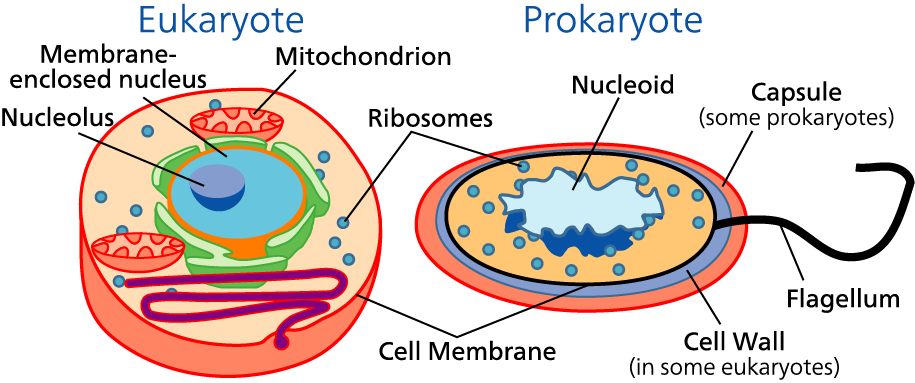
\includegraphics[width=0.75\textwidth]{fig01/prokaryote_and_eukaryote_cells.png}
  \caption{Eukaryotic and prokaryotic cells (source: \href{https://commons.wikimedia.org/wiki/File:Celltypes.svg}{Science Primer, Wikimedia Commons})}
\end{figure}

\noindent \textbf{2. Cell size –- around 1 to 100 micrometers}
\begin{itemize}
\item Cell Size and Scale: \url{http://learn.genetics.utah.edu/content/cells/scale}
\end{itemize}
\medskip  

\noindent \textbf{3. The number of cells}
\begin{itemize}
\item Prokaryotes: 1 cell
\item Human:  Estimate of 15 trillion cells
\end{itemize}
\medskip 

\noindent \textbf{4. An animal cell and cell organelles}
\begin{figure}[H]
  \centering
      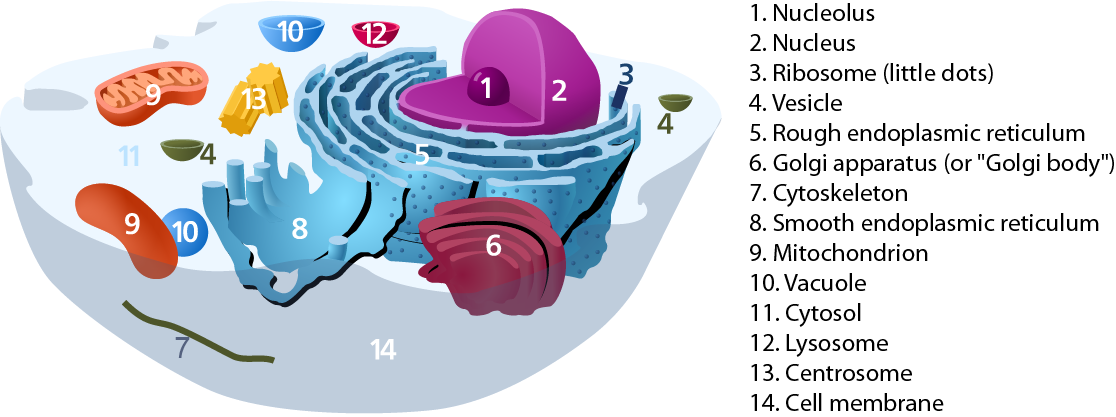
\includegraphics[width=0.75\textwidth]{fig01/animal_cells_and_organelles.png}
  \caption{An animal cell and organelles (source: \href{https://en.wikipedia.org/wiki/Organelle\#/media/File:Animal_Cell.svg}{Kelvinsong, Wikimedia Commons})}
\end{figure}

\noindent \textbf{5. Cellular processes}
\begin{itemize}
\item Cell growth, cell development, cell signaling, …
\item Example: \url{http://www.nature.com/nrg/multimedia/rnai}
\end{itemize}

%
% Central dogma of molecular biology
%
\subsubsection*{Central dogma of molecular biology}

It describes the information flow within a cell.

\begin{figure}[H]
  \centering
      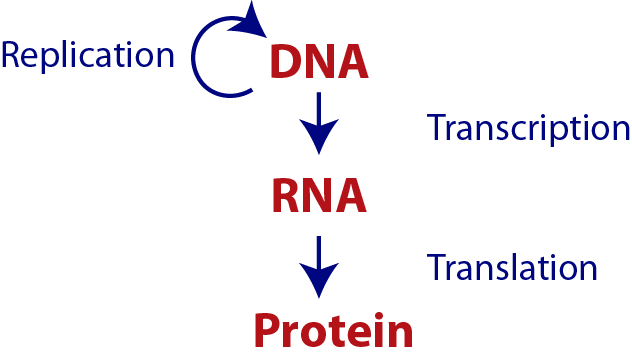
\includegraphics[width=0.75\textwidth]{fig01/central_dogma_of_molecular_biology.png}
  \caption{Central dogma of molecular biology}
\end{figure}

%
% DNA (deoxyribonucleic acid)
%
\subsubsection*{DNA (deoxyribonucleic acid)}

DNA stores genetic information. It has four different bases: cytosine (C), guanine (G), adenine (A), and thymine (T).

\begin{figure}[H]
  \centering
      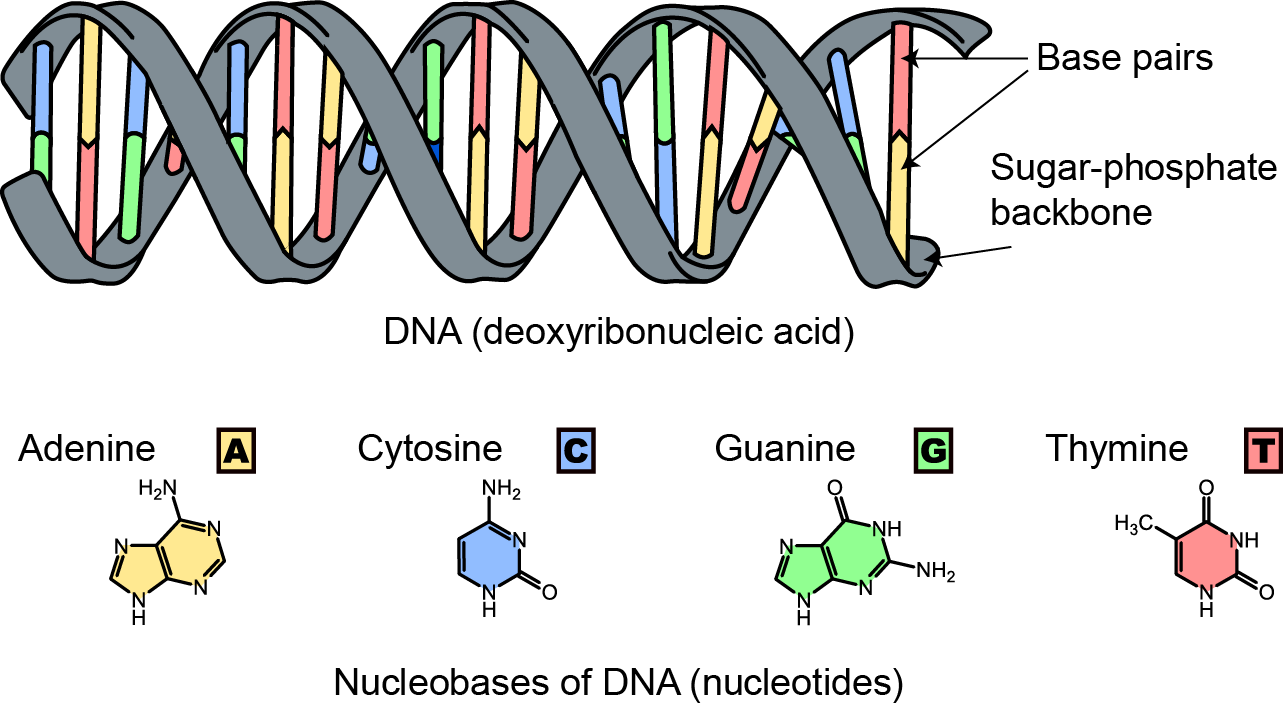
\includegraphics[width=0.5\textwidth]{fig01/dna_bases.png}
  \caption{DNA double helix and base pairs \newline (modified from the original version by \href{https://commons.wikimedia.org/w/index.php?curid=9810855}{Sponk, Wikimedia Commons})}
\end{figure} 

\noindent \textbf{Base pair matching (Watson-Crick base pair)}

\noindent Adenine (A) pairs with thymine (T), whereas cytosine (C) pairs with guanine (G).

\begin{verbatim}
DNA strand1: ACGT
             ||||
DNA strand2: TGCA
\end{verbatim}
	
%
% RNA (Ribonucleic acid)
%
\subsubsection*{RNA (Ribonucleic acid)}
RNA has various biological roles and several sub-classes. Messenger RNAs (mRNAs) convey genetic information.  It has four different bases: cytosine (C), guanine (G), adenine (A), and uracil (U).

\begin{figure}[H]
  \centering
      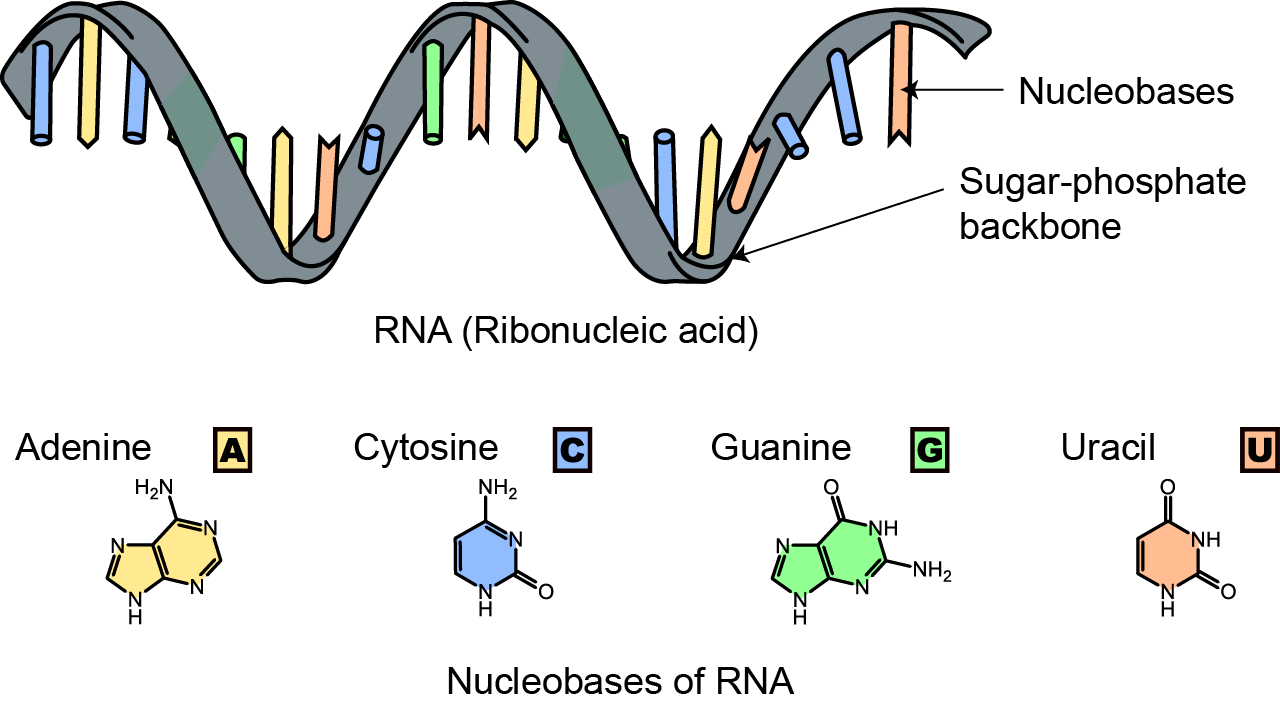
\includegraphics[width=0.5\textwidth]{fig01/rna_bases.png}
  \caption{Single strand RNA \newline (modified from the original version by \href{https://commons.wikimedia.org/w/index.php?curid=9810855}{Sponk, Wikimedia Commons})}
\end{figure}

\noindent \textbf{Transcription: mRNAs are transcribed from DNAs}

\begin{verbatim}
DNA: ACGT -------> RNA: ACGU
        Transcription
\end{verbatim}

%
% Protein
%
\subsubsection*{Protein}

Proteins are large molecules consisting of amino acids. There are 20 common amino acids.
 
\begin{figure}[H]
  \centering
      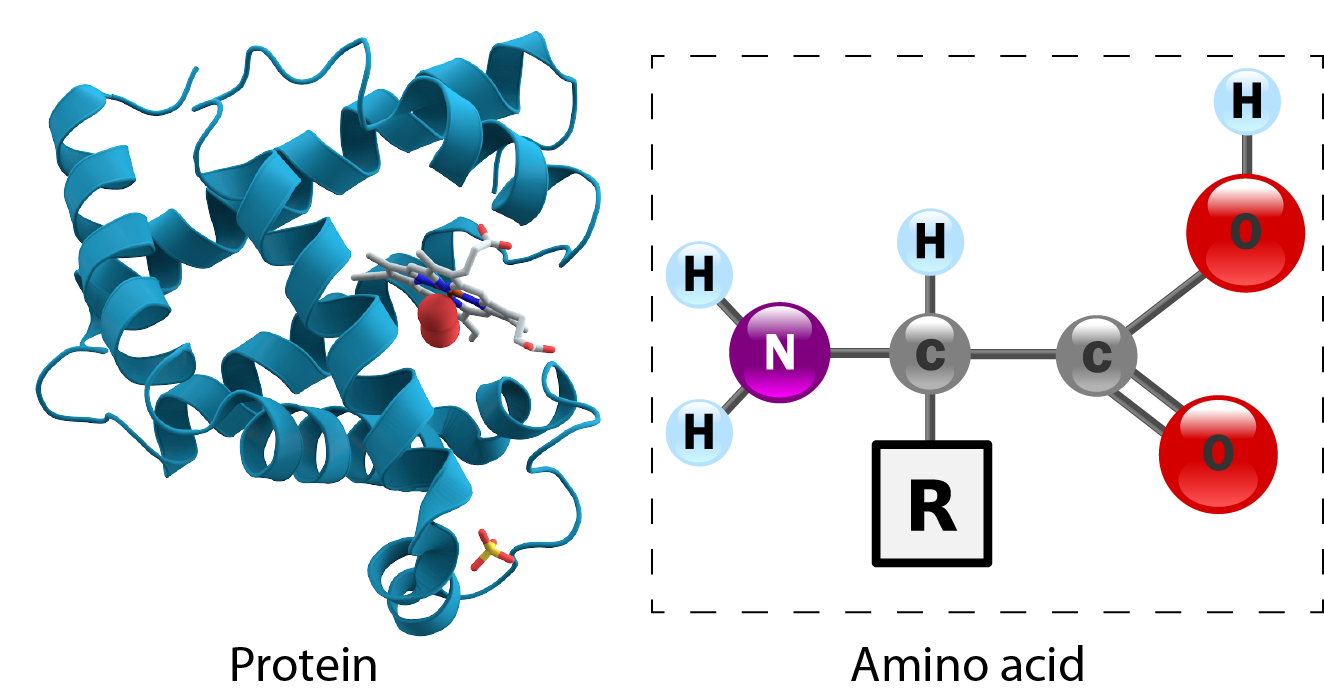
\includegraphics[width=0.6\textwidth]{fig01/protein_and_amino_acid.png}
  \caption{Protein 3D structure and amino acids \newline (sources: \href{https://en.wikipedia.org/wiki/Protein\#/media/File:Myoglobin.png}{AzaToth, Wikimedia Commons}, \href{https://en.wikipedia.org/wiki/Amino_acid\#/media/File:AminoAcidball.svg}{YassineMrabet, Wikimedia Commons})}
\end{figure}

\noindent \textbf{Translation: Amino-acids are translated from mRNAs}

\begin{verbatim}
mRNA: GUC -------> AA: Valine
        Translation
\end{verbatim}

\newpage 

\noindent \textbf{Universal genetic code}

\noindent A codon consists of three nucleic acids. Single-letter or three-letter names can be used for amino acids.

\begin{figure}[H]
  \centering
      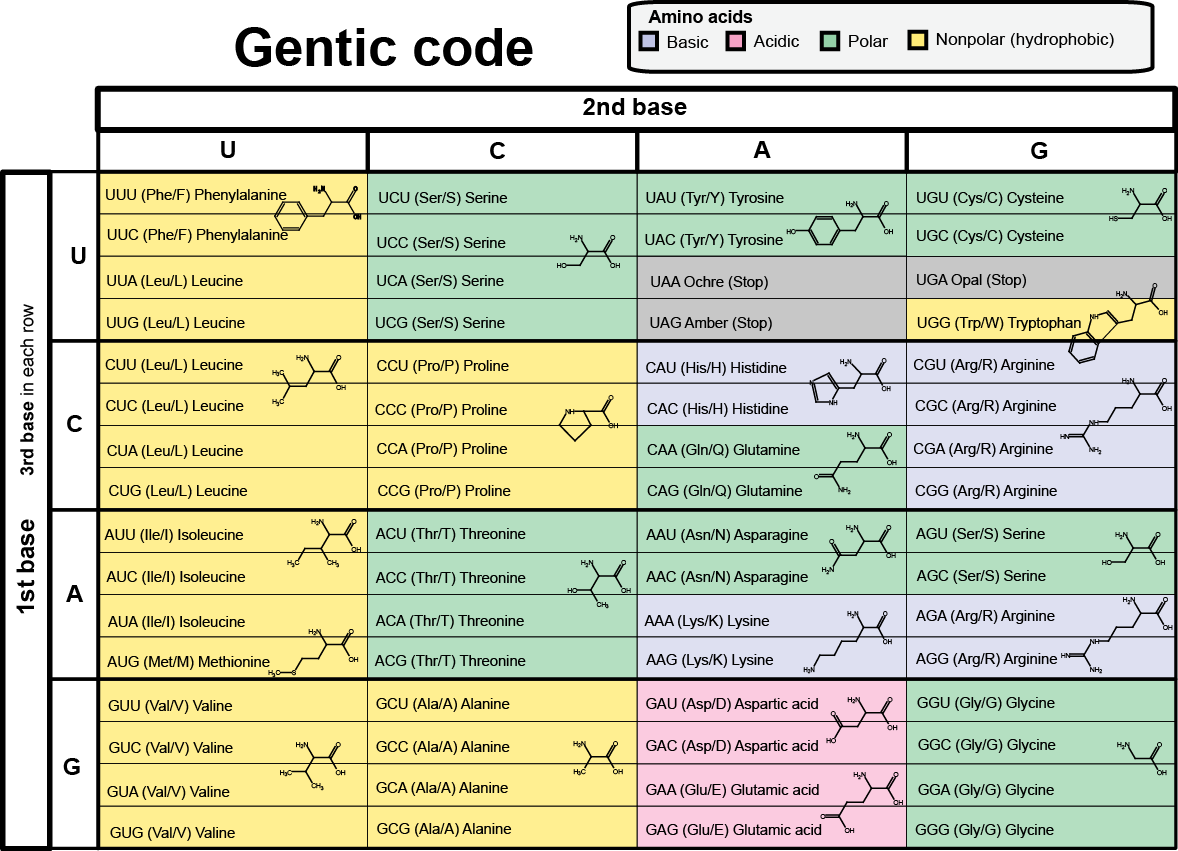
\includegraphics[width=0.7\textwidth]{fig01/genetic_code.png}
  \caption{Universal genetic code \newline (modified from the original version by \href{https://commons.wikimedia.org/wiki/File\%3ANotable_mutations.svg}{H\"aggstr\"om, Wikimedia Commons})}
\end{figure}

\noindent \textbf{Cellular functions of proteins}
\begin{itemize}
\item Enzymes: catalyze chemical reaction
\item Cell signaling: hormone (e.g. insulin), antibodies, …
\item Structural: collagen, cartilage, keratin, …
\end{itemize}

%
% Exercises 1.1
%
\subsubsection*{Exercises 1.1}
\begin{enumerate}

\item Draw a simple diagram of the central dogma of molecular biology and briefly explain the information flow of the molecules.

\item What are the DNA sequences of the opposite strand for the following DNA sequences?
\begin{verbatim}
    Seq1 CCGATT
    Seq2 TTACGC
    Seq3 ACGCGC
\end{verbatim}

\item What are the mRNA sequences transcribed from the following DNA sequences?

\item What are the polypeptide sequences translated from the following mRNA sequences? Answer them with both one-letter and three letter names.
\begin{verbatim}
    Seq1 AUGUUUUAA
    Seq2 GCAGCAAAA
\end{verbatim}
		
\end{enumerate}

%\end{document}

%\documentclass[12pt]{article}
%\usepackage[a4paper, margin=1in]{geometry} 
%\usepackage{graphicx} 
%\usepackage{hyperref}
%\usepackage{float}
%\usepackage[font=small, labelfont=bf]{caption}

%\begin{document}

%
% Introduction to Biotechnology
%
\subsection{Introduction to Biotechnology}
Biotechnology is the use of laboratory techniques to study living organism and cells. 

%
% Applications of biotechnology
%
\subsubsection*{Applications of biotechnology}
Branches of biotechnology can be explained with different colors.
\begin{itemize}
\item Red: medical processes
\item Green: agricultural processes
\item White: industrial processes
\item Blue: marine and aquatic applications
\end{itemize}

%
% Laboratory tools and equipment
%
\subsubsection*{Laboratory tools and equipment}

\begin{figure}[H]
  \centering
      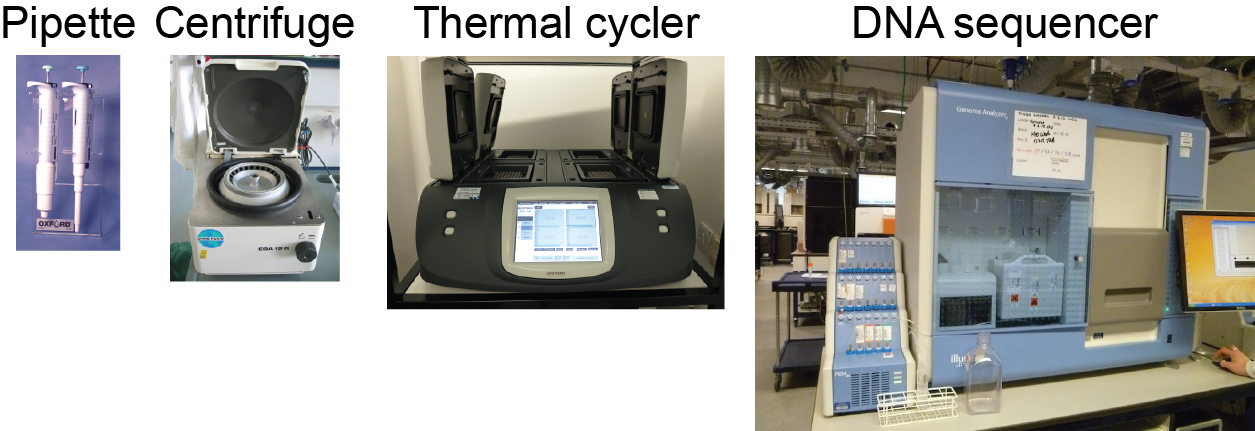
\includegraphics[width=0.5\textwidth]{fig01/lab_equipment.png}
  \caption{Pipette, centrifuge, thermal cycler, and DNA sequencer \newline (sources:  \href{https://en.wikipedia.org/wiki/Pipette\#/media/File:Single_channel_rack.jpg}{Domain}, \href{https://commons.wikimedia.org/w/index.php?curid=494}{Manske},
\href{https://commons.wikimedia.org/w/index.php?curid=20189025}{Rror}, 
\href{https://commons.wikimedia.org/w/index.php?curid=18862968}{RE73} via Wikimedia Commons)}
\end{figure}
 
%
% Human genome project
%
\subsubsection*{Human genome project}
It was a large-scale international research project to determine the whole DNA sequences of human.

\begin{itemize}
\item 1990 –- 2003
\item \$2.7 billion
\end{itemize}

%
% Next generation sequencing
%
\subsubsection*{Next generation sequencing}
Sequence technologies have been rapidly advanced since the human genome project.

Example: sequence a whole human genome with Illumina HiSeq X Ten.
\begin{itemize}
\item One day
\item \$1000
\end{itemize}

%
% Protein sequencing
%
\subsubsection*{Protein sequencing}
Proteins are generally more studied than DNAs and RNAs, but the whole proteome is generally harder to analyze than the whole genome. MS (mass-spectrometry) based technologies are widely used to sequence proteins.

\begin{figure}[H]
  \centering
      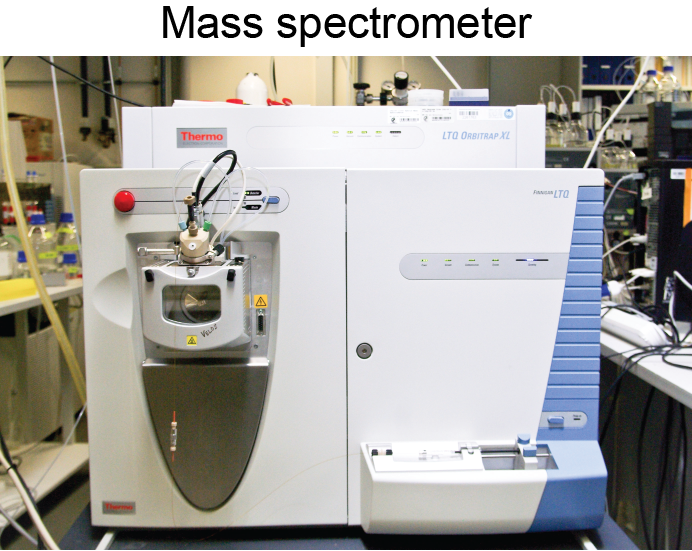
\includegraphics[width=0.25\textwidth]{fig01/mass_spectrometer.png}
  \caption{Orbitrap mass spectrometer (source: \href{https://commons.wikimedia.org/w/index.php?curid=18691799}{Wi\`{o}rkiewicz, Wikimedia Commons})}
\end{figure}
 
%\end{document}

%\documentclass[12pt]{article}
%\usepackage[a4paper, margin=1in]{geometry} 
%\usepackage{graphicx} 
%\usepackage{hyperref}
%\usepackage{float}
%\usepackage[font=small, labelfont=bf]{caption}
%
%\begin{document}

%
% Bioinformatics in INF281
%
\subsection{Bioinformatics in INF281}
Bioinformatics uses computational approaches to solve problems in life sciences. It is based on computer science.

%
% Similar or almost equivalent disciplines
%
\subsubsection*{Similar or almost equivalent disciplines}
\begin{itemize}
\item Biostatistics
\item Biophysics
\item Systems biology
\item Computational biology
\end{itemize}

%
% Not much related with bioinformatics
%
\subsubsection*{Not much related with bioinformatics}
\begin{itemize}
\item Health informatics
\item Forensic science
\end{itemize}

%
% Scope of INF281
%
\subsubsection*{Scope of INF281}
We mainly cover the following fields of bioinformatics in this course.
\begin{itemize}
\item Pairwise alignment
\item Database search
\item Statistical evaluation
\item Multiple alignment
\item Phylogenetic tree
\item Scoring scheme
\item Sequence patterns
\end{itemize}

%
% Popular bioinformatics programs
%
\subsubsection*{Popular bioinformatics programs}
BLAST and ClustalW are popular tools for sequence analysis.
\begin{itemize}
\item BLAST: a program for database search

URL: \url{http://blast.ncbi.nlm.nih.gov}

\item ClustalW: a program for multiple alignments

URL: \url{http://www.ch.embnet.org/software/ClustalW.html}

\end{itemize}

\begin{table}[!ht]
\scriptsize

\begin{tabular}{l p{10cm} r}
Rank & Title& Times cited \\
\hline
1 & Protein measurement with the folin phenol reagent & 305148 \\
2 & Cleavage of structural proteins during the assembly of the head of bacteriophage T4 & 213005 \\
3 & A rapid and sensitive method for the quantitation of microgram quantities of protein utilizing the principle of protein-dye binding & 155530 \\
4 & DNA sequencing with chain-terminating inhibitors & 65335 \\
5 & Single-step method of RNA isolation by acid guanidinium thiocyanate-phenol-chloroform extraction & 60397 \\
6 & Electrophoretic transfer of proteins from polyacrylamide gels to nitrocellulose sheets: procedure and some applications & 53349 \\
7 & Development of the Colle-Salvetti correlation-energy formula into a functional of the electron density & 46702 \\
8 & Density-functional thermochemistry. III. The role of exact exchange & 46145 \\
9 & A simple method for the isolation and purification of total lipides from animal tissues & 45131 \\
\textbf{10} & \textbf{Clustal W}: improving the sensitivity of progressive multiple sequence alignment through sequence weighting, position-specific gap penalties and weight matrix choice & 40289 \\
11 & Nonparametric estimation from incomplete observations & 38600 \\
\textbf{12} & \textbf{Basic local alignment search tool} & 38380 \\
13 & A short history of SHELX & 37978 \\
\textbf{14} & \textbf{Gapped BLAST and PSI-BLAST}: A new generation of protein database search programs & 36410 \\
15 & A revised medium for rapid growth and bio assays with tobacco tissue cultures & 36132 \\
\end{tabular}
\caption{The 15 most cited papers of all time \newline (The top 100 papers, Van Noorden, Maher, and Nuzzo, \textit{Nature}, 2014)}
\end{table}

%\end{document}


\newpage

%
% PART II
%
\part{}

%
% Global_pairwise_alignment
%
\setcounter{figure}{0}
\setcounter{table}{0}
\section{Global pairwise alignment}
%\documentclass[12pt]{article}
%\usepackage[a4paper, margin=1in]{geometry} 
%\usepackage{graphicx} 
%\usepackage{hyperref}
%\usepackage{float}
%\usepackage{multicol}
%\usepackage[font=small, labelfont=bf]{caption}
%
%\begin{document}

%
% Pairwise alignment
%
\subsection{Pairwise alignment}
A pairwise alignments is a basic sequence structure that consits of two sequences. A global alignment stretches to the whole part of two sequences, whereas a local alignment usually contains only part of the sequences.

%
% Pairwise alignment
%
\subsubsection*{Components of pairwise alignment}

We name two sequences as ‘database’ or ‘d’ and ‘query’ or ‘q’ through this course. They may represent sequences from two different species or organisms.
\\

\noindent
Identical sequences.
\begin{verbatim}
    q: ACGT
    d: ACGT
\end{verbatim}

\noindent
One mismatch.
\begin{verbatim}
    q: ACGT
    d: ACGA
\end{verbatim}

\noindent
The '-' symbol represents a blank. A single or a set of multile blanks further reprents a gap, which is an indication of insertion or deletion in the course of evoluation between two organisms.
\begin{verbatim}
    q: ACGT
    d: A-GT
\end{verbatim}

\noindent
\textbf{N.B.} A gap cannot be aligned with another gap.

%
% Example of a simple scoring scheme
%
\subsubsection*{Example of a simple scoring scheme}
\begin{itemize}
\item Match: 1
\item Mismatch: 0
\item Gap penalty: 1 (use -1 for the actual calculation)
\end{itemize}

\noindent
We may use the following notation.
\begin{itemize}
\item $R_{ab}$ = 1 for a = b
\item $R_{ab}$ = 0 for a $\neq$ b
\item g = 1
\end{itemize}

%
% NEW PAGE
%
\newpage 

%
% Exercise \thesection.1
%
\subsubsection*{Exercise \thesection.1}
Use the simple scoring scheme above and calculate the scores of the following two alignments.

\begin{multicols}{2}
\begin{verbatim}
Alignment 1
    q: GCA-GCA
    d: GA-TG-A	
\end{verbatim}

\begin{verbatim}
Alignment 2 
    q: GCA-GCA
    d: GA-TG-A	
\end{verbatim}
\end{multicols}

%\end{document}

%\documentclass[12pt]{article}
%\usepackage[a4paper, margin=1in]{geometry} 
%\usepackage{graphicx} 
%\usepackage{hyperref}
%\usepackage{float}
%\usepackage{multicol}
%\usepackage[font=small, labelfont=bf]{caption}
%
%\begin{document}

%
% Alignment by brute-force
%
\subsection{Alignment by brute--force}
A brute--force approach finds the alignment with the highest score by simply considering all possible alignments and calculates the score for each of them.

%
% An example of brute--force approach
%
\subsubsection*{An example of brute--force approach}
We find the optimal alignment for the following sequences by using the scoring scheme below.

\begin{multicols}{2}
Sequences:
\begin{verbatim}
    q: AG, d: ACG
\end{verbatim}
\vfill\null
\columnbreak

\noindent Scoring scheme: \\ 
\null \quad $R_{ab}$ = 1 for a = b \\ 
\null \quad $R_{ab}$ = 0 for a $\neq$ b \\ 
\null \quad g = 1

\end{multicols} 

\noindent \textbf{1. The length of alignment}
\begin{itemize}
\item Maximum length: length(q) + length(d)
\item Minimum length: max(length(q), length(d))
\end{itemize}
\medskip 

\noindent \textbf{2. All possible alignments when length = 5}
\begin{verbatim}
    ---AG    A---G    A--G-    AG---    --A-G
    ACG--    -ACG-    -AC-G    --ACG    AC-G-

    --AG-    -AG--    -A--G    -A-G-    A-G--
    AC--G    A--CG    A-CG-    A-C-G    -A-CG
\end{verbatim}
\medskip

\noindent \textbf{3. All possible alignments when length = 4}
\begin{verbatim}
    A--G    A-G-    AG--    A--G    -A-G    -AG-
    ACG-    AC-G    A-CG    -ACG    ACG-    AC-G

    -AG-    A-G-    --AG    --AG    -A-G    AG--
    A-CG    -ACG    ACG-    AC-G    A-CG    -ACG
\end{verbatim}
\medskip

\noindent \textbf{4. All possible alignments when length = 3}
\begin{verbatim}
    -AG    A-G    AG-
    ACG    ACG    ACG
\end{verbatim}
\medskip

\noindent \textbf{5. Alignment with the best score}
\begin{verbatim}
    ACG
    A-G	
\end{verbatim}

Score: 1

%
% Search space size of the brute-force approach
%
\subsubsection*{Search space size of the brute-force approach}
The search space size is the number of all possible alignments. It is 25 (10 + 12 + 3) for the example above. \\

\noindent \textbf{Rapid growth of search space size}

\begin{multicols}{2}
\begin{verbatim}
Example 1
    q: ACGACG, d: AGAG
\end{verbatim}
Search space size: 1289

\begin{verbatim}
Example 2
    q: ACGACGACGACG, d: AGAGAGAG
\end{verbatim}
Search space size: 4,673,345

\end{multicols}

%
% Exercise \thesection.2
%
\subsubsection*{Exercise \thesection.2}
Find the alignment with the best score for the sequences.  Use the simple scoring scheme below.

\begin{multicols}{2}
Sequences:
\begin{verbatim}
    q: A, d: AC
\end{verbatim}
\vfill\null
\columnbreak

\noindent Scoring scheme: \\ 
\null \quad $R_{ab}$ = 1 for a = b \\ 
\null \quad $R_{ab}$ = 0 for a $\neq$ b \\ 
\null \quad g = 1

\end{multicols} 

\begin{enumerate}
\item What are the maximum and minimum lengths of the alignment?
\item Identify all possible alignments.
\item What is the best score?
\item What is the search space size when the brute-force approach is used?
\end{enumerate}

%\end{document}

%\documentclass[12pt]{article}
%\usepackage[a4paper, margin=1in]{geometry} 
%\usepackage{graphicx} 
%\usepackage{hyperref}
%\usepackage{float}
%\usepackage{multicol}
%\usepackage[font=small, labelfont=bf]{caption}
%
%\begin{document}

%
% Alignment by brute-force
%
\subsection{Table representation of alignment}
Several data strcutres can be used to repesent an alignment. The table representation is frequently used and also makes the process clear when we combine it with dynamic programming (DP) later.

\subsubsection*{Data structures and algorithms}
It is important to consider the following aspects before solving computational problems.
\begin{enumerate}
\item Identify and analyze the problem you want to solve
\item Pick up an algorithm that can efficiently solve the problem
\item Decide a data structure that works with the algorithm of your choice
\end{enumerate}

\noindent We use a table format (2D array) to solve global alignments by dynamic programming.

\subsubsection*{Example of table format}
Alignment:
\begin{verbatim}
    q: -AG-
    d: A-CG
\end{verbatim}
\medskip 

\noindent \textbf{1. Initial setup}

\begin{enumerate}
\item Make a table with the size of (1 + length(q)) by (1 + length(b))
\item Add the database sequence as column labels
\item And the query sequence as row labels
\end{enumerate}

\begin{figure}[H]
  \centering
      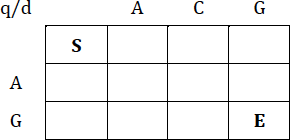
\includegraphics[width=0.3\textwidth]{fig02/alignment_to_table.png}
\end{figure}

\noindent \textbf{2. Add arrows}

We use three types of arrows to form an alignment.
\begin{itemize}
\item Move diagonally: add the letters from ‘q’ and ‘d’ to the alignment
\item Move vertically: add ‘-’ and the letter from ‘d’ to the alignment
\item Move horizontally: add the letter from ‘q’ and ‘-’ to the alignment
\end{itemize}

It shoud start from S and stops at E.

\begin{figure}[H]
  \centering
      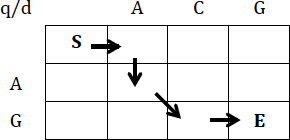
\includegraphics[width=0.3\textwidth]{fig02/alignment_to_table_example.png}
\end{figure}

%
% Exercise \thesection.3
%
\subsubsection*{Exercise \thesection.3}

Find the corresponding alignments for Table 1, 2 and 3.

\begin{multicols}{3}
Table 1
\begin{figure}[H]
  \centering
      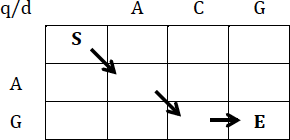
\includegraphics[width=0.3\textwidth]{fig02/alignment_to_table_exercise1.png}
\end{figure}

Table 2
\begin{figure}[H]
  \centering
      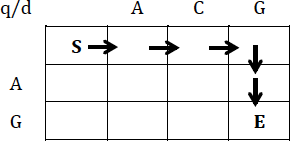
\includegraphics[width=0.3\textwidth]{fig02/alignment_to_table_exercise2.png}
\end{figure}

Table 3
\begin{figure}[H]
  \centering
      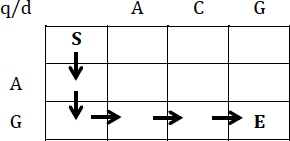
\includegraphics[width=0.3\textwidth]{fig02/alignment_to_table_exercise3.png}
\end{figure}

\end{multicols} 

%\end{document}

%\documentclass[12pt]{article}
%\usepackage[a4paper, margin=1in]{geometry} 
%\usepackage{graphicx} 
%\usepackage{hyperref}
%\usepackage{float}
%\usepackage{multicol}
%\usepackage{amsmath}
%\usepackage[ruled]{algorithm2e}
%\usepackage[font=small, labelfont=bf]{caption}
%
%\begin{document}

%
% Global alignment with DP
%
\subsection{Global alignment with DP}
Dynamic programming (DP) provides a solution for a multi-stage decision process, in which larger decisions recursively nest smaller decisions.

\subsubsection*{Memorize the best score in a table cell}

The most basic step of DP procedures is updatig a cell with the hightet score from the three different scores calculated from its adjacent cells. DP ends when all the table cells are updated.

\begin{figure}[H]
  \centering
      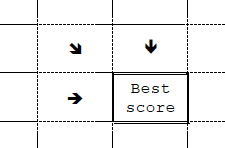
\includegraphics[width=0.25\textwidth]{fig02/dynamic_programmoing_cell_update.png}
\end{figure}

%
% Table notation and indices
%	
\subsubsection*{Table notation and indices}
$H_{i,j}$ represents the score of the cell for the current update. $H_{i-1,j}$, $H_{i,j-1}$,and $H_{i-1,j-1}$ are the scores of the adjacent cells.

\begin{multicols}{2}

Cell $H_{i, j}$ and its adjcent cells
\begin{figure}[H]
  \centering
      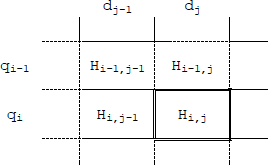
\includegraphics[width=0.3\textwidth]{fig02/dynamic_programmoing_cell_indices.png}
\end{figure}

Example
\begin{figure}[H]
  \centering
      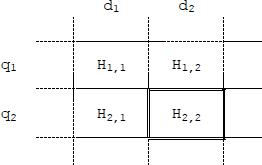
\includegraphics[width=0.3\textwidth]{fig02/dynamic_programmoing_cell_indices_example.png}
\end{figure}

\end{multicols} 

%
% Calculation of three candidate scores
%	
\subsubsection*{Calculation of three candidate scores}
$H_{i,j}^{(0)}$, $H_{i,j}^{(1)}$, and $H_{i,j}^{(2)}$ represent the three candidate scores of $H_{i,j}$. They are respectively calculated as:
\begin{align*}
H_{i,j}^{(0)} &= H_{i-1,j} - g &(vertical) \\
H_{i,j}^{(1)} &= H_{i,j-1} - g	&(horizontal) \\
H_{i,j}^{(2)} &= H_{i-1,j-1} + R_{a,b} &(diagonal)
\end{align*}

%
% Exercise \thesection.4
%
\subsubsection*{Exercise \thesection.4}

Calculate the scores of $H_{4,6}^{(0)}$, $H_{4,6}^{(1)}$, and $H_{4,6}^{(2)}$ first and then update $H_{4,6}$.
\begin{multicols}{2}
\begin{figure}[H]
  \centering
      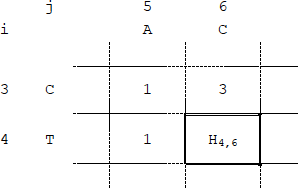
\includegraphics[width=0.3\textwidth]{fig02/dynamic_programmoing_cell_update_exercise.png}
\end{figure}

\noindent Scoring scheme: \\ 
$R_{ab}$ = 1 for a = b \\ 
$R_{ab}$ = 0 for a $\neq$ b \\ 
g = 1

\end{multicols} 

%
% Initialization
%
\subsubsection*{Initialization}

The first row and the first column can be calcuated independently from the adjcent cells.
\begin{align*}
H_{0,j} &:  j * -1 * g \\
H_{i,0} &: i * -1 * g
\end{align*}

\noindent
Example
\begin{figure}[H]
  \centering
      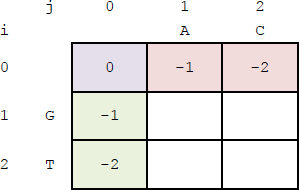
\includegraphics[width=0.3\textwidth]{fig02/dynamic_programmoing_initialization.png}
\end{figure}

%
% Exercise \thesection.5
%
\subsubsection*{Exercise \thesection.5}
Update all cells of Table 1 and 2. Use the scoring scheme in Exercise \thesection.4.

\begin{multicols}{2}
Table 1
\begin{figure}[H]
  \centering
      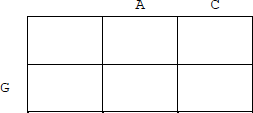
\includegraphics[width=0.3\textwidth]{fig02/global_alignment_exercise1.png}
\end{figure}

\vfill\null
\columnbreak

Table 2
\begin{figure}[H]
  \centering
      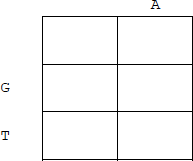
\includegraphics[width=0.25\textwidth]{fig02/global_alignment_exercise2.png}
\end{figure}

\end{multicols} 

%
% Sub-solutions
%
\subsubsection*{Sub-solutions}

In DP, larger decisions recursively nest smaller decisions. For instance, Table S is included in Table L.

\begin{multicols}{2}
Table S
\begin{figure}[H]
  \centering
      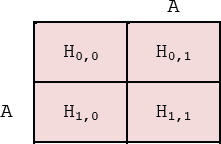
\includegraphics[width=0.3\textwidth]{fig02/dynamic_programmoing_subsolution_S.png}
\end{figure}

\vfill\null
\columnbreak

Table L
\begin{figure}[H]
  \centering
      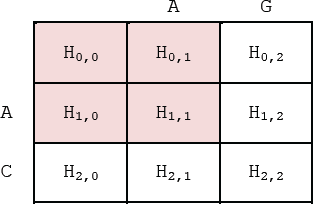
\includegraphics[width=0.4\textwidth]{fig02/dynamic_programmoing_subsolution_L.png}
\end{figure}

\end{multicols} 

%
% NEW PAGE
%
\newpage

%
% Psedo-code of global alignment with DP
%
\subsubsection*{Psedo-code of updating DP table for global alignment}

\begin{algorithm}[H]
  \SetKwInOut{HAB}{$\mathrm{H_{i,j}}$}
  \SetKwInOut{RAB}{$\mathrm{R_{a,b}}$}
  \SetKwInOut{G}{$\mathrm{g}$}
  \SetKwData{dRAB}{$\mathrm{R_{a,b}}$}
  \SetKwData{dG}{$\mathrm{g}$}
  
  \BlankLine
    
  \HAB{Dyanamic programming table}
  \RAB{Match/mismatch scores}
  \G{Gap penalty}
  
  \BlankLine \BlankLine
  
  \tcp{Initialization}
  \For{$i \leftarrow 0$ \KwTo $m$}{
    $\mathrm{H_{i,0}}$ $\leftarrow$ $i * -1 * g$\;
  }
  \For{$j \leftarrow 1$ \KwTo $n$}{
    $\mathrm{H_{0,j}}$ $\leftarrow$ $j * - 1 * g$\;
  }
  
  \BlankLine \BlankLine
    
  \tcp{Main loop for table update}
  \For{$i \leftarrow 1$ \KwTo $m$}{
    \For{$j \leftarrow 1$ \KwTo $n$}{
      $\mathrm{H_{i,j}}$ $\leftarrow$ $max(\mathrm{H_{i-1,j}} - \dG, \mathrm{H_{i,j-1}} - \dG, \mathrm{H_{i-1,j-1}}$ + \dRAB)\;
    }
  }
  
  \SetAlgoRefName{\thesection.1}
  \caption{Update dynamic programming table for global alignment}

\end{algorithm}

%\end{document}

%\documentclass[12pt]{article}
%\usepackage[a4paper, margin=1in]{geometry} 
%\usepackage{graphicx} 
%\usepackage{hyperref}
%\usepackage{float}
%\usepackage{multicol}
%\usepackage{amsmath}
%\usepackage[ruled]{algorithm2e}
%\usepackage{amssymb}
%\usepackage[font=small, labelfont=bf]{caption}

%\begin{document}

%
% Backtracking
%
\subsection{Backtracking}
Backtracking is a post-processing procedure to find the alignments that have yielded the best score. 

%
% Store movement in cells
%
\subsubsection*{Store movement in cells}

A table cell can be used for storing the movement.
\begin{figure}[H]
  \centering
      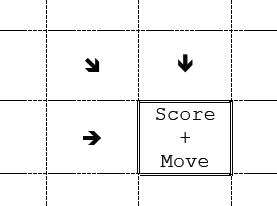
\includegraphics[width=0.3\textwidth]{fig02/back_tracking_store_moves.png}
\end{figure}

\noindent \textbf{Example}
\begin{multicols}{2}
Cells with scores and directions
\begin{figure}[H]
  \centering
      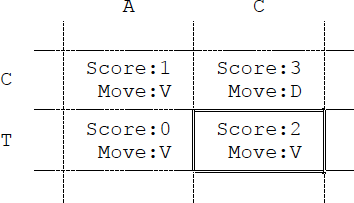
\includegraphics[width=0.3\textwidth]{fig02/back_tracking_store_moves_example.png}
\end{figure}

Use arrows to indicate backtracking
\begin{figure}[H]
  \centering
      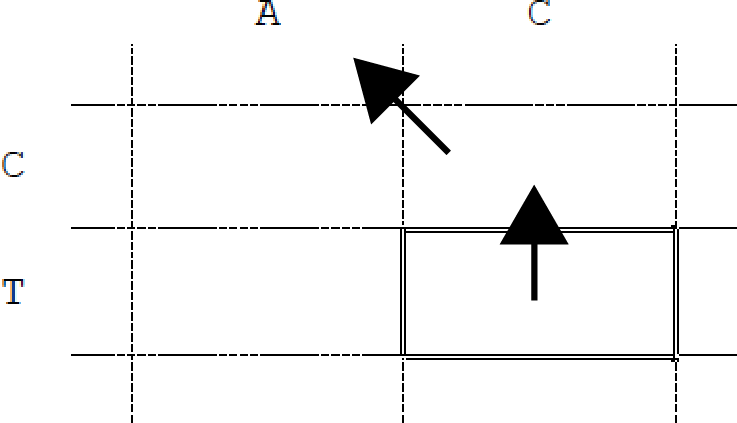
\includegraphics[width=0.3\textwidth]{fig02/back_tracking_store_moves_arrows.png}
\end{figure}

\end{multicols} 

%
% Exercise \thesection.6
%
\subsubsection*{Exercise \thesection.6}
	
Complete the DP table with scores and directions. What is the alignment with the best score?

\begin{multicols}{2}
\begin{figure}[H]
  \centering
      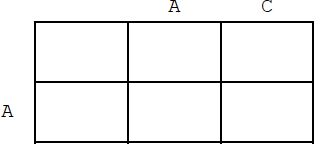
\includegraphics[width=0.3\textwidth]{fig02/back_tracking_store_moves_exercise.png}
\end{figure}

\noindent Scoring scheme: \\ 
$R_{ab}$ = 1 for a = b \\ 
$R_{ab}$ = 0 for a $\neq$ b \\ 
g = 1

\end{multicols} 

%
% Re-calculate candidate scores
%
\subsubsection*{Re-calculate candidate scores}

Re-calculating the three candidate scores also reveals the movement.

\begin{align*}
H_{i,j}^{(0)} &= H_{i-1,j} - g &(vertical) \\
H_{i,j}^{(1)} &= H_{i,j-1} - g &(horizontal) \\
H_{i,j}^{(2)} &= H_{i-1,j-1} + R_{a,b} &(diagonal)
\end{align*}

\noindent \textbf{Example}

\begin{figure}[H]
  \centering
      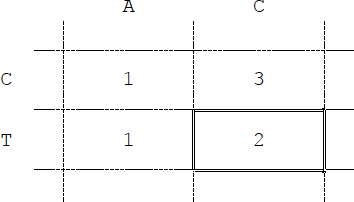
\includegraphics[width=0.3\textwidth]{fig02/back_tracking_example.png}
\end{figure}
				
\begin{align*}
H_{i,j}^{(0)} &= 3 - 1 = 2 = H_{i,j} &\checkmark & (vertical) \\
H_{i,j}^{(1)} &= 1 - 1 = 0 \neq H_{i,j} &\hfill & (horizontal) \\
H_{i,j}^{(2)} &= 1 + 0 = 1 \neq H_{i,j} &\hfill  & (diagonal)
\end{align*}

%
% Common mistake with backtracking
%
\subsubsection*{Common mistake with backtracking}
For the re-calculation approach, it is not to find $max(H_{i-1,j}, H_{i,j-1}, H_{i-1,j-1})$. You must re-calculate the candidates and then $max(H_{i,j}^{(0)}, H_{i,j}^{(1)} , H_{i,j}^{(2)})$ to find the actual direction.

%
% Implementation with recursive call
%
\subsubsection*{Implementation with recursive call}
Recursive calls are usually used to implement DP backtracking.

\begin{algorithm}[H]
  \SetKwInOut{HAB}{$\mathrm{H_{i,j}}$}
  \SetKwInOut{RAB}{$\mathrm{R_{a,b}}$}
  \SetKwInOut{G}{$\mathrm{g}$}
  
  \SetKwProg{Fn}{proc}{}{end}
  \SetKwInOut{I}{$\mathrm{i}$}
  \SetKwInOut{J}{$\mathrm{j}$}
  \SetKwInOut{SQ}{$\mathrm{S_{q}}$}
  \SetKwInOut{SD}{$\mathrm{S_{d}}$}
  \SetKwInOut{AQ}{$\mathrm{A_{q}}$}
  \SetKwInOut{AD}{$\mathrm{A_{d}}$}
  \SetKwInOut{K}{$\mathrm{k}$}

  \SetKwData{dI}{$\mathrm{i}$}
  \SetKwData{dJ}{$\mathrm{j}$}
  \SetKwData{dAQ}{$\mathrm{A_{q}}$}
  \SetKwData{dAD}{$\mathrm{A_{d}}$}
  \SetKwData{dK}{$\mathrm{k}$}
    
  \SetKwData{dRAB}{$\mathrm{R_{a,b}}$}
  \SetKwData{dG}{$\mathrm{g}$}

  \BlankLine
  
  \SQ{Sequence q}
  \SD{Sequence d}     
  \HAB{Dynamic programming table}
  \RAB{Match/mismatch scores}
  \G{Gap penalty}

  \BlankLine \BlankLine

  \Fn{backTrack(\dI, \dJ, \dAQ, \dAD, \dK)}{
    
    \BlankLine
    
    \I{Index of sequence q}
    \J{Index of sequence d}
    \AQ{q part of alignment (stored in reverse order)}
    \AD{d part of alignment (stored in reverse order)}
    \K{Index for \dAQ and \dAD}
  
    \BlankLine
    
    \tcp{}
    \tcp{Need to implement recursion termination here}
    \tcp{...}
    \tcp{}
        
    \BlankLine
    
    \If(\tcp*[f]{vertical}){$\mathrm{H_{i,j}} = \mathrm{H_{i-1,j}} - g$}{
      $\mathrm{A_{q, k}} $ $\leftarrow$ $ S_{q, i}$\;
      $\mathrm{A_{d, k}} $ $\leftarrow$ $ $ '-'\;
      $backTrack$($\mathrm{i-1}$, \dJ, \dAQ, \dAD, $k + 1$)\;
    }
    \BlankLine

    \If(\tcp*[f]{horizontal}){$\mathrm{H_{i,j}} = \mathrm{H_{i,j-1}} - g$}{
      $\mathrm{A_{q, k}} $ $\leftarrow$ '-'\;
      $\mathrm{A_{d, k}} $ $\leftarrow$ $ S_{d, i}$\;
      $backTrack$(\dI, $\mathrm{j-1}$, \dAQ, \dAD, $k + 1$)\;
    }
    \BlankLine
    
    \If(\tcp*[f]{diagonal}){$\mathrm{H_{i,j}} = \mathrm{H_{i-1,j-1}} +\mathrm{R_{S_{q, i},S_{d, i}}}$}{
      $\mathrm{A_{q, k}} $ $\leftarrow$ $ S_{q, i}$\;
      $\mathrm{A_{d, k}} $ $\leftarrow$ $ S_{d, i}$\;
      $backTrack$($\mathrm{i-1}$, $\mathrm{j-1}$, \dAQ, \dAD, $k + 1$)\;
    }
      
    \BlankLine
  }

  \SetAlgoRefName{\thesection.2}
  \caption{DP backtracking}

\end{algorithm}

%
% Exercise \thesection.7
%
\subsubsection*{Exercise \thesection.7}
	
Find the alignment with the best score.

\begin{multicols}{2}
\begin{figure}[H]
  \centering
      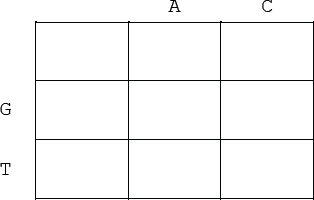
\includegraphics[width=0.3\textwidth]{fig02/back_tracking_exercise.png}
\end{figure}

\noindent Scoring scheme: \\ 
$R_{ab}$ = 1 for a = b \\ 
$R_{ab}$ = 0 for a $\neq$ b \\ 
g = 1

\end{multicols} 

%\end{document}

%\documentclass[12pt]{article}
%\usepackage[a4paper, margin=1in]{geometry} 
%\usepackage{graphicx} 
%\usepackage{hyperref}
%\usepackage{float}
%\usepackage{multicol}
%\usepackage{amsmath}
%\usepackage[ruled]{algorithm2e}
%\usepackage{amssymb}
%\usepackage[font=small, labelfont=bf]{caption}
%
%\begin{document}

%
% Needleman-Wunsch
%
\subsection{Needleman-Wunsch algorithm}
The method of using DP to solve global pairwise alignment is called the Needleman-Wunsch algorithm in the field of bioinformatics. 

%
% Complexity
%
\subsubsection*{Complexity}
\begin{itemize}
\item Time: O(nm)
\item Space: O(nm)
\end{itemize}

%
% Comparisons with other algorithms
%
\subsubsection*{Comparisons with other algorithms}
The Needleman-Wunsch algorithm is similar to several algorithms.
\\

\noindent
\textbf{Divide and conquer algorithms}

\noindent
Sub-solutions must be independent with divide and conquer.

\begin{figure}[H]
  \centering
      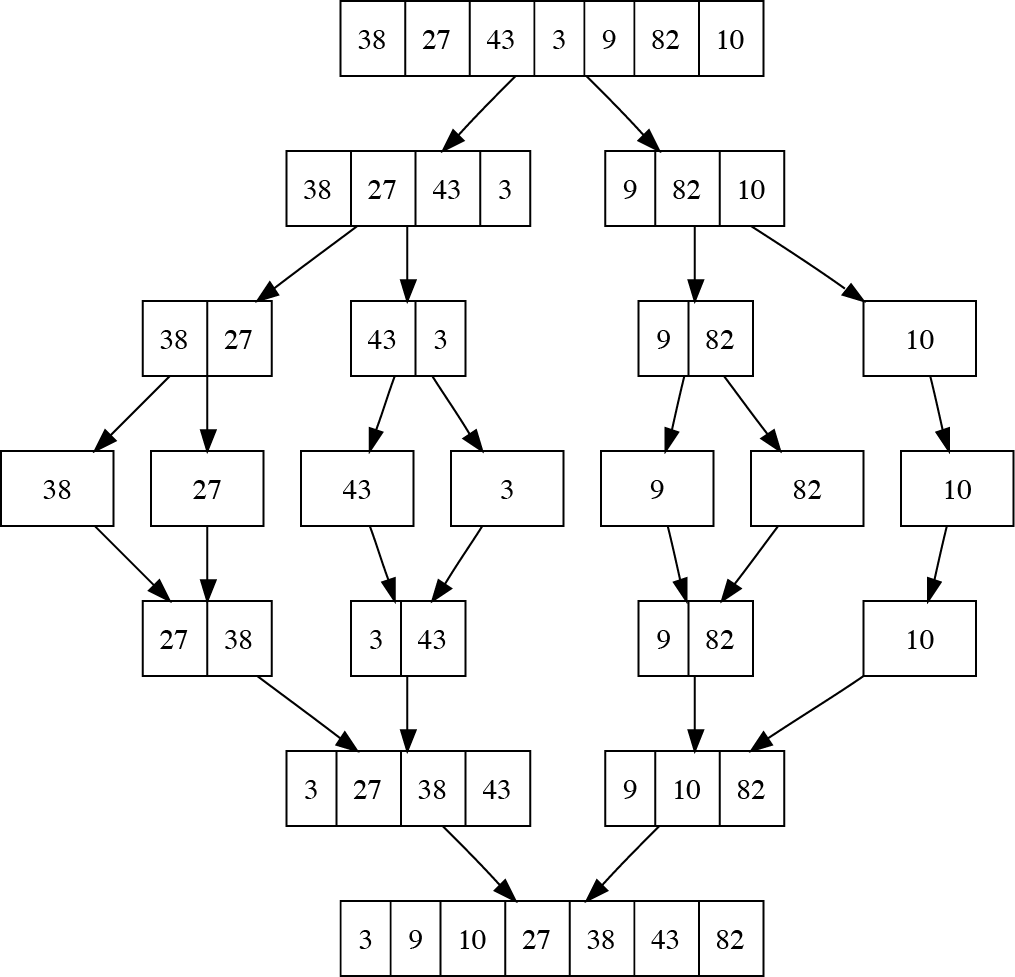
\includegraphics[width=0.25\textwidth]{fig02/Merge_sort_algorithm.png}
  \caption{Merge sort (source: \href{https://commons.wikimedia.org/w/index.php?curid=8004317}{VineetKumar, Wikimedia Commons})}
\end{figure}

\noindent
\textbf{Dijkstra's algorithm}

\noindent
Worst-case performance of Dijkstra: $O(|E|+|V|\log |V|)$

\begin{figure}[H]
  \centering
      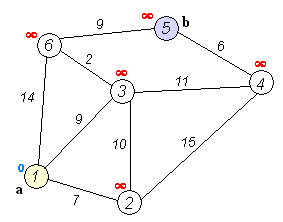
\includegraphics[width=0.25\textwidth]{fig02/Dijkstra.png}
  \caption{Dijkstra's algorithm (source: \href{https://commons.wikimedia.org/w/index.php?curid=6282617}{Ibmua, Wikimedia Commons})}
\end{figure}

%\end{document}


\newpage

%
% Extension_of_global_alignment
%
\setcounter{figure}{0}
\setcounter{table}{0}
\section{Extension of global alignment}
%\documentclass[12pt]{article}
%\usepackage[a4paper, margin=1in]{geometry} 
%\usepackage{graphicx} 
%\usepackage{hyperref}
%\usepackage{float}
%\usepackage{multicol}
%\usepackage[font=small, labelfont=bf]{caption}
%
%\begin{document}

%
% Homology at the sequence level
%
\subsection{Homology at the sequence level}
Constructing alignments can be useful to understand homology among different species. Finding homologies is important to reveal a common evolutionary ancestor.

%
% Evolution and homology
%
\subsubsection*{Evolution and homology}
All species are derived from a common ancestor at some point during the course of evolution.
 
\begin{figure}[H]
  \centering
      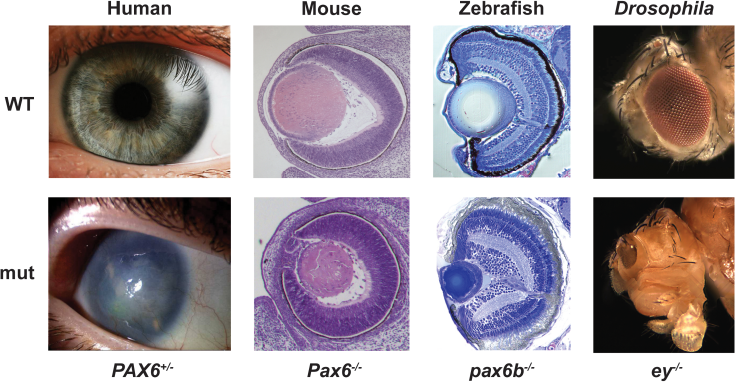
\includegraphics[width=0.5\textwidth]{fig03/PAX6_mutation.png}
  \caption{PAX6 alterations result in similar changes to eye morphology \newline (source: Washington et al, doi: 10.1371/journal.pbio.1000247 via \href{https://commons.wikimedia.org/w/index.php?curid=8626896}{Wikimedia Commons})}
\end{figure}

%
% Homologous and  analogous
%
\subsubsection*{Homologous and  analogous}
It is useful to check similarity at the molecular level because there are cases that analogous structures may not indicate homologous. 
\begin{figure}[H]
  \centering
      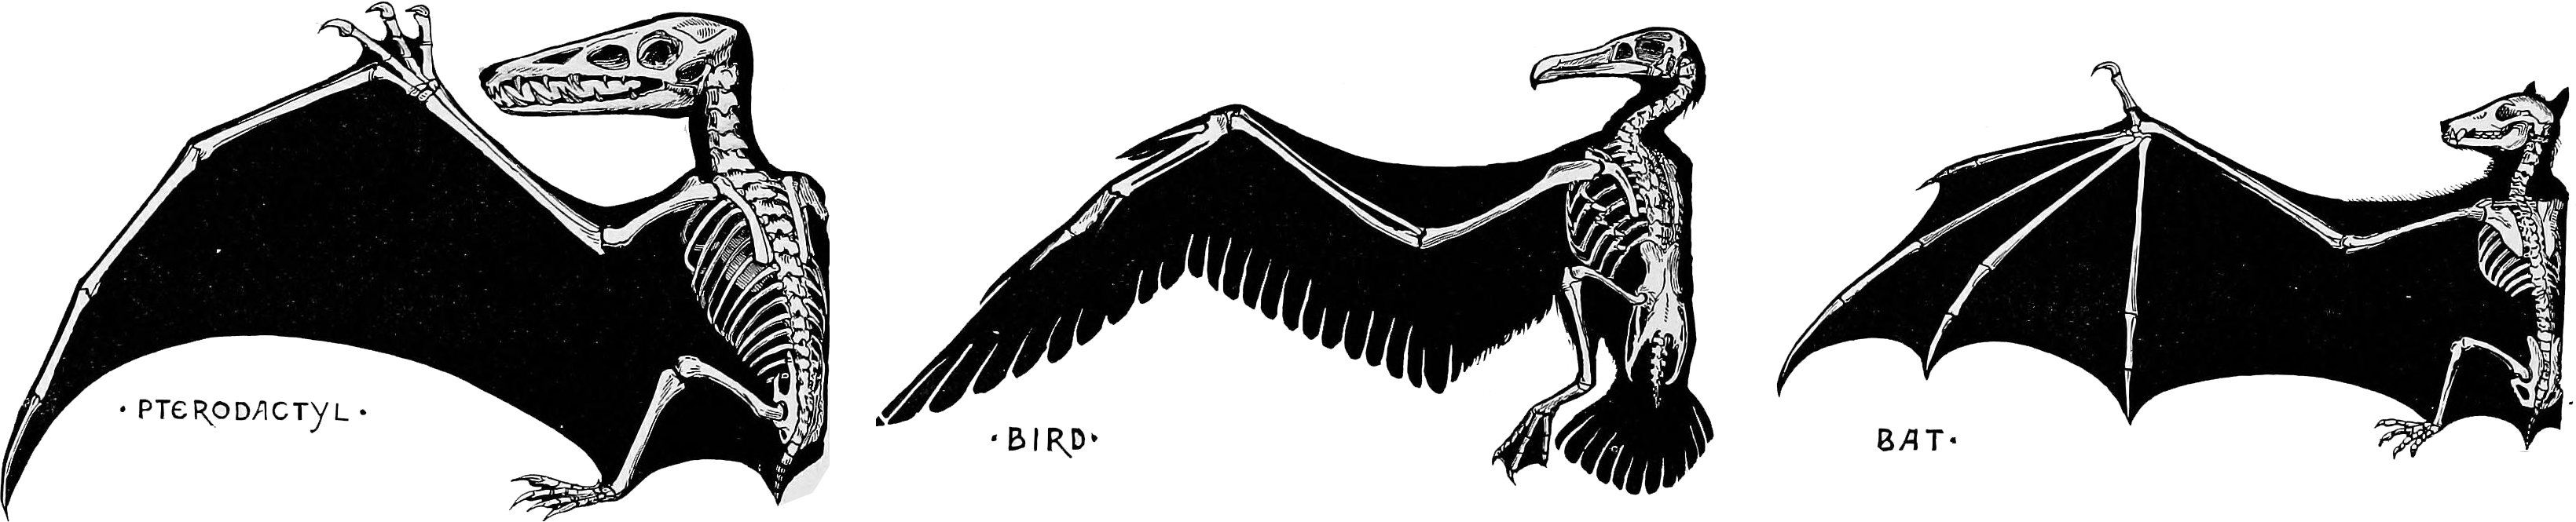
\includegraphics[width=0.5\textwidth]{fig03/analogous.png}
  \caption{Homologous and  analogous structures \newline (source: John Romanes, 1892, Darwin and after Darwin via \href{https://commons.wikimedia.org/w/index.php?curid=1324636}{Wikimedia Commons})}
\end{figure}

%
% Sequence homology
%
\subsubsection*{Sequence homology}
\begin{figure}[H]
  \centering
      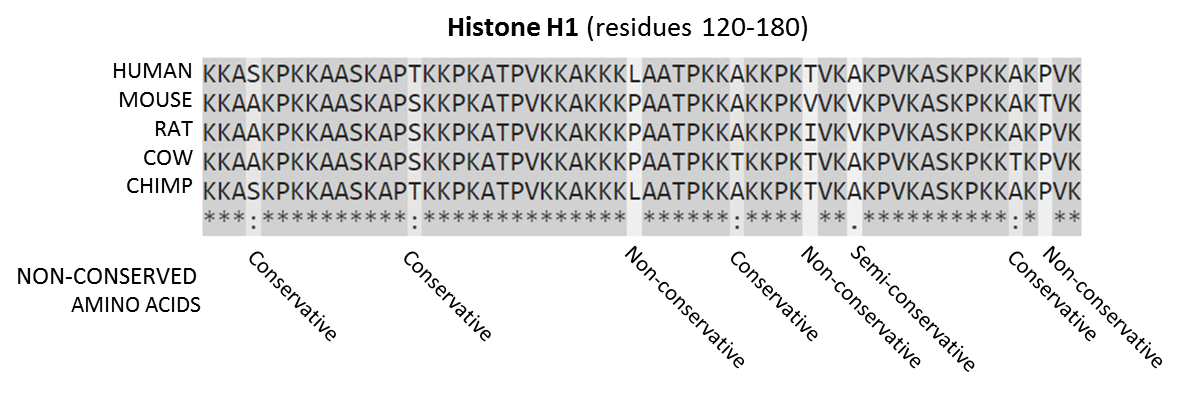
\includegraphics[width=0.75\textwidth]{fig03/histone_alignment.png}
  \caption{Multiple sequence alignment of histon sequences \newline (source: \href{https://commons.wikimedia.org/w/index.php?curid=37188728}{Shafee, Wikimedia Commons})}
\end{figure}

%
% Sequence homology
%
\subsubsection*{Evolution at the sequence level}
Sequence differences in DNA
\begin{itemize}
\item Substitution (a mismatch in alignment)
\item Insertion (a gap in alignment)
\item Deletion (a gap in alignment)
\item Inversion
\end{itemize}

\noindent
Source of variations
\begin{itemize}
\item Mutation
\item Recombination
\item Insertional mutagenesis
\item ...
\end{itemize}

\noindent
A mutation of the third nucleotide in a codon often does not affect which amino acid is synthesized.
\begin{itemize}
\item GCU $\rightarrow$ Ala (Alanine)
\item GCC $\rightarrow$ Ala (Alanine)
\item GCA $\rightarrow$ Ala (Alanine)
\item GCG $\rightarrow$ Ala (Alanine)
\end{itemize}

\noindent
An amino acid can be replaced by a different amino acid that has similar properties in some cases.
\begin{itemize}
\item AUU, AUC, AUA $\rightarrow$ Ile (Isoleucine)
\item CUU, CUC, CUA $\rightarrow$ Leu (Leucine)
\end{itemize}

%
% Extension of global alignment
%
\subsubsection*{Extension of global alignment with DP}

\begin{itemize}
\item Score matrix \\
DNA, RNA, and protein

\item Gap penatlty \\
Linear, affine, and constant
\end{itemize}



%\end{document}

%\documentclass[12pt]{article}
%\usepackage[a4paper, margin=1in]{geometry} 
%\usepackage{graphicx} 
%\usepackage{hyperref}
%\usepackage{float}
%\usepackage{multicol}
%\usepackage[font=small, labelfont=bf]{caption}
%
%\begin{document}

%
% Introduction of score matrix
%
\subsection{Introduction of score matrix}
We will expand our simple scoring scheme to score matrices. This expansion allows us to solve general alignment problems with DNA, RNA, and protein sequences. 

%
% Extension of a scoring scheme to a score matrix
%
\subsubsection*{Extension of a scoring scheme to a score matrix}
The matrix below is equivalent with match: 1 and mismatch: 0. 

\begin{figure}[H]
  \centering
      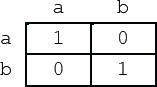
\includegraphics[width=0.175\textwidth]{fig03/simple_score_matrix.png}
\end{figure}

\noindent
\textbf{Example of a DNA score matrix}

\noindent
The matrix below is equivalent with match: 5 and mismatch: -4. 

\begin{figure}[H]
  \centering
      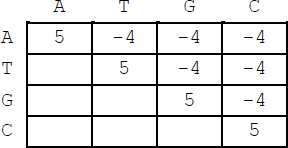
\includegraphics[width=0.3\textwidth]{fig03/dna_matrix_exercise.png}
\end{figure}

%
% Applications of score matrix
%
\subsubsection*{Applications of score matrix}

Score matrices are more flexible than the simple scoring scheme. For instance, they can be used for the following cases.

\begin{itemize}
\item DNA pairs
\item RNA pairs
\item Similarity of protein sequences by amino acid properties
\end{itemize}

%
% DNA pairs (Watson-Crick pairs)
%
\subsubsection*{DNA pairs (Watson-Crick pairs)}
A thymine pairs with an adenine, and a cytosine pairs with a guanine.

\begin{figure}[H]
  \centering
      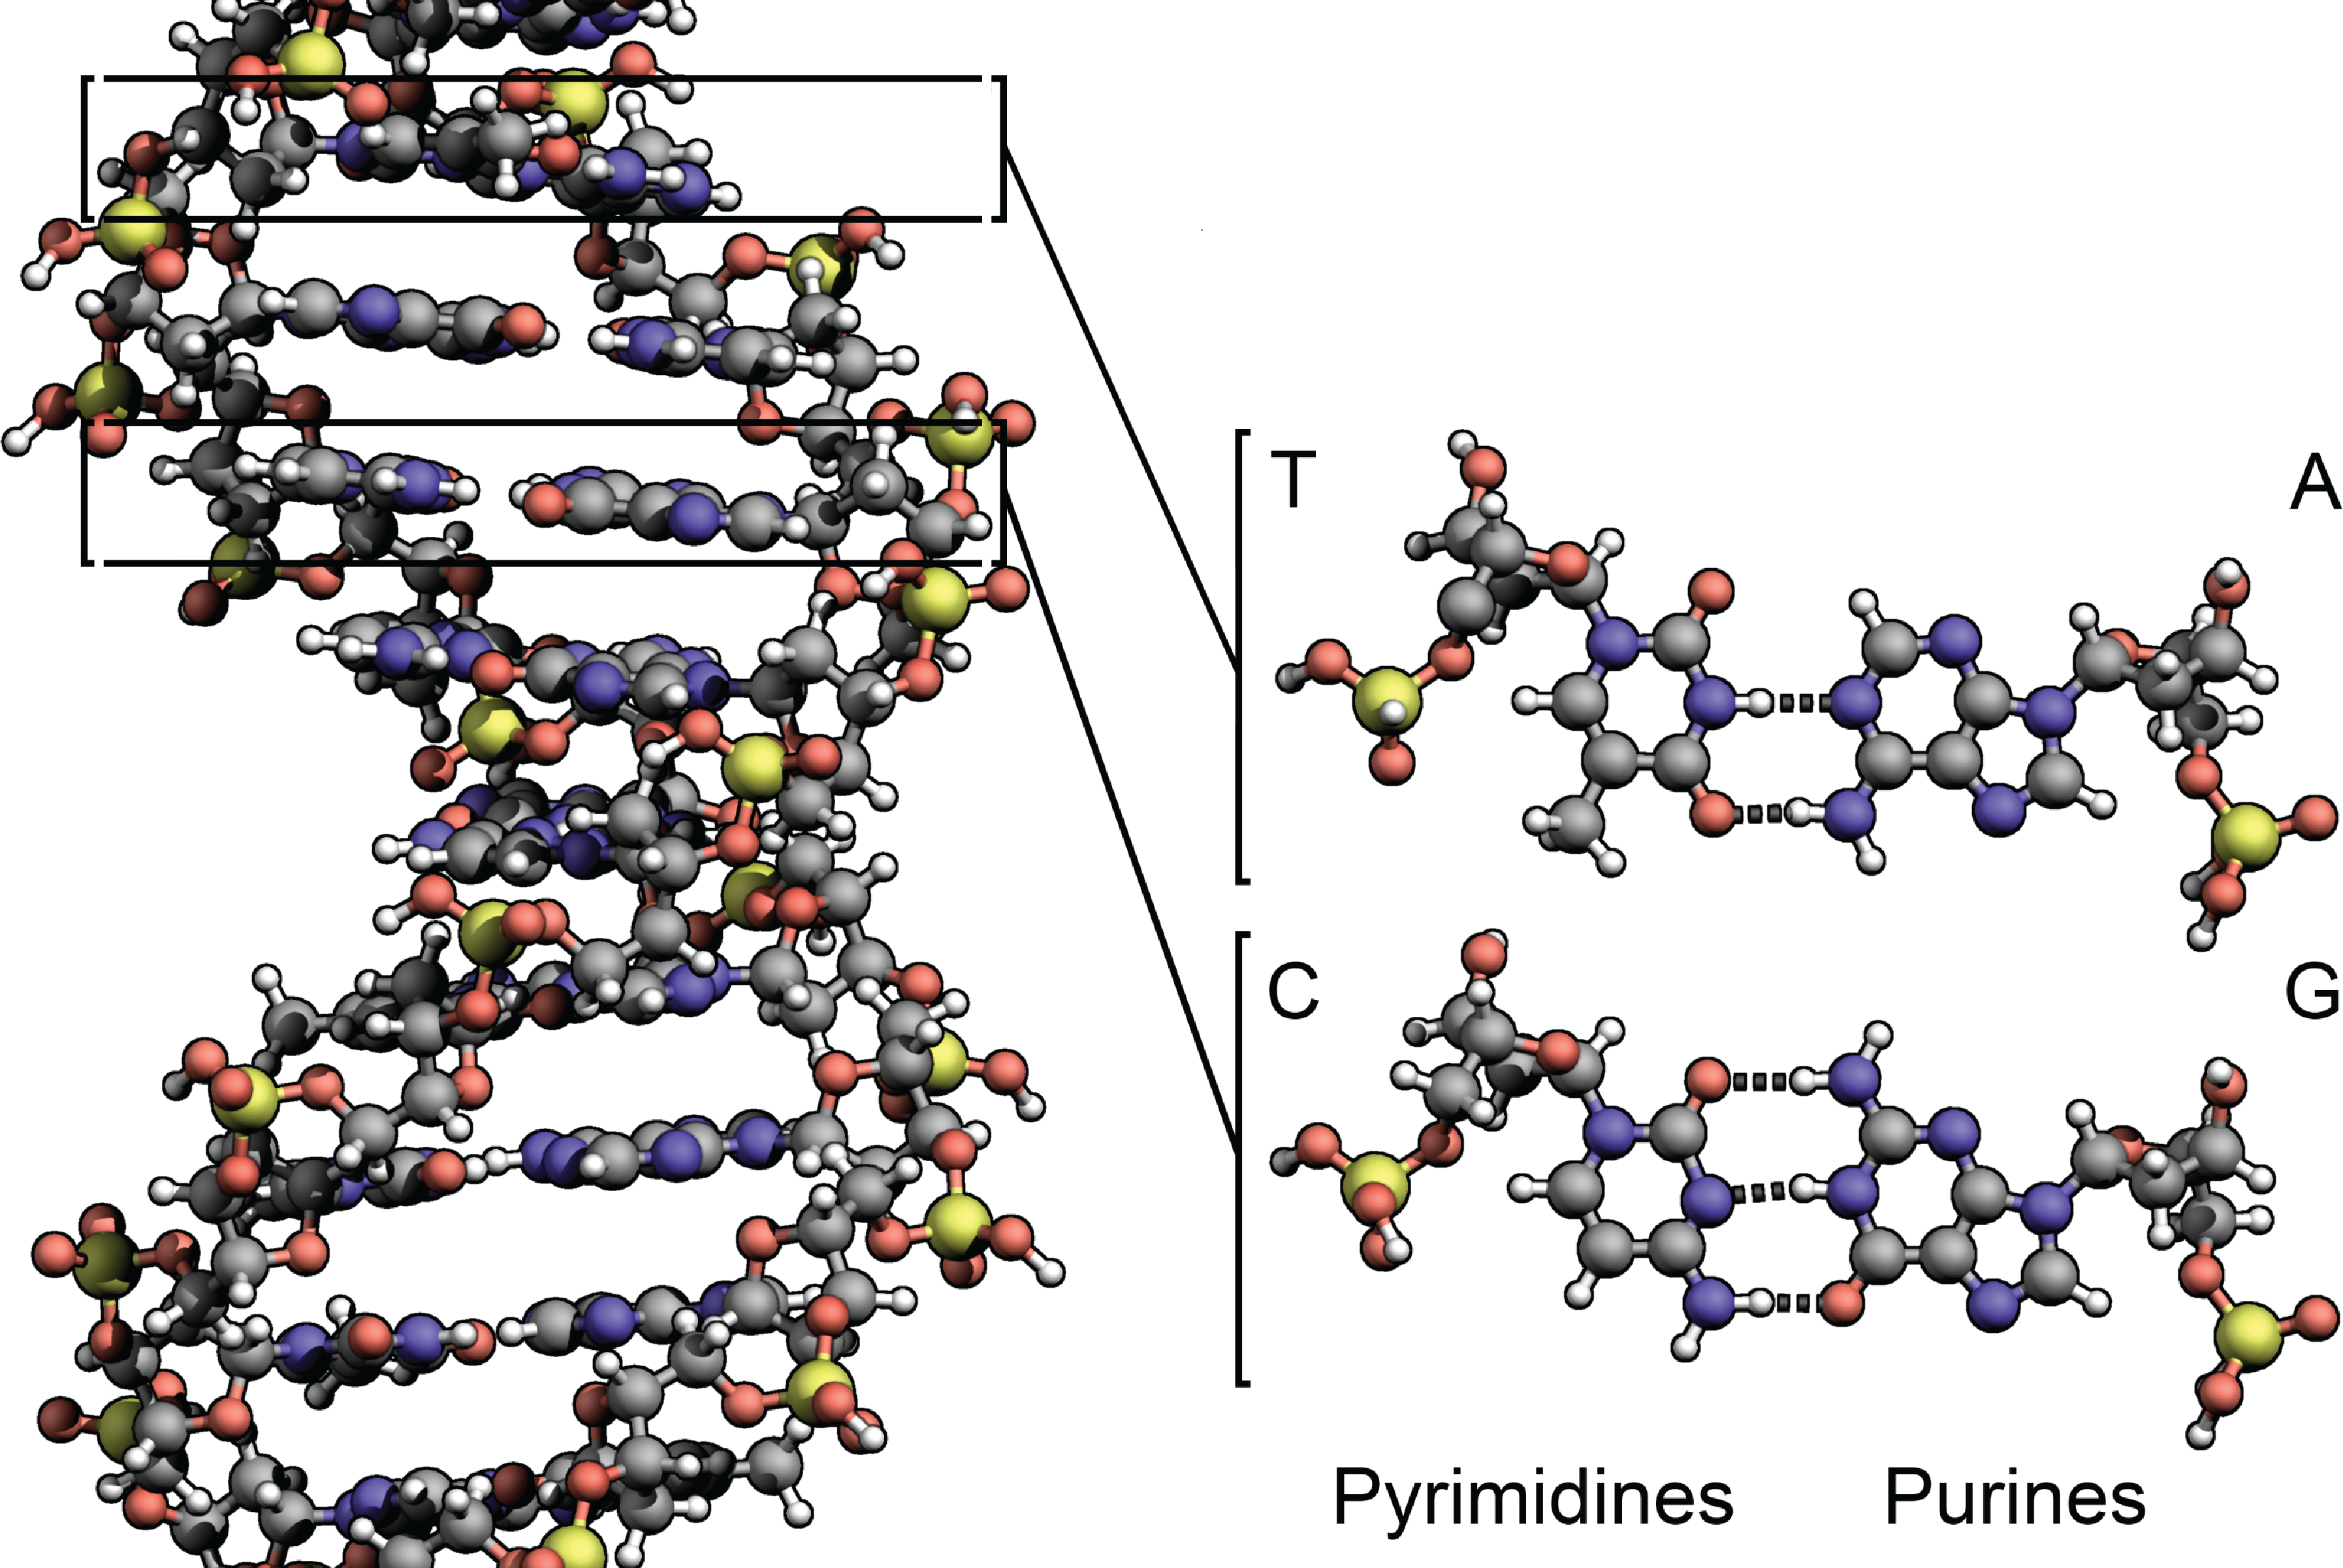
\includegraphics[width=0.4\textwidth]{fig03/dna_watson_crick_pair.png}
  \caption{Watson-Crick pairs (source: \href{https://commons.wikimedia.org/w/index.php?curid=15027555}{Zephyris, Wikimedia Commons})}
\end{figure}

%
% NEWPAGE
%
\newpage

\noindent \textbf{Example of score matrix for DNA pairs} \\
\noindent The matrix reflects the difference of hydrogen bonds.

\begin{figure}[H]
  \centering
      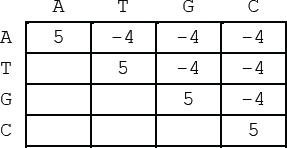
\includegraphics[width=0.3\textwidth]{fig03/example_dna_score_matrix.png}
\end{figure}

\noindent \textbf{Example of DP for DNA pairs} \\
\noindent You can use DP to find a DNA alignment with Watson-Crick pairs. For instance, the DP table below is used to solve the optimal alignment for two DNA sequences: q = AC and d = GT with gap penalty g = 4.

\begin{multicols}{2}
DP table:
\begin{figure}[H]
  \centering
      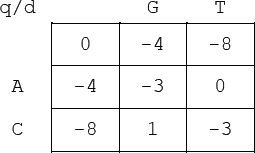
\includegraphics[width=0.25\textwidth]{fig03/example_watson_crick_alignment.png}
\end{figure}

Alignment:
\begin{verbatim}
    q: AC-
    d: -GT
\end{verbatim}

\end{multicols} 

%
% RNA pairs (Watson-Crick pairs)
%
\subsubsection*{RNA pairs}
A single stand of RNA can form a 3D structure that has a biological function. The secondary structure of RNA is a two-dimensional representation of the structure. 

\begin{figure}[H]
  \centering
      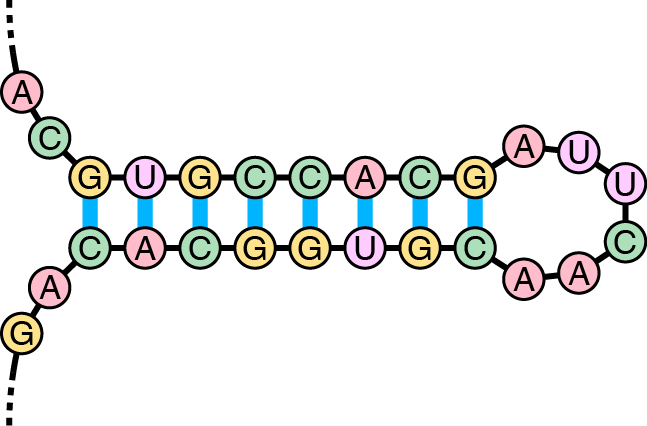
\includegraphics[width=0.3\textwidth]{fig03/rna_stem_loop.png}
  \caption{RNA stem-loop (source: \href{https://commons.wikimedia.org/w/index.php?curid=815268}{Sakurambo, Wikimedia Commons})}
\end{figure}

\noindent \textbf{Wobble pairs} \\
\noindent Wobble pairs are not canonical Watson-Crick pairs, but they can still form hydrogen bonds.

\begin{figure}[H]
  \centering
      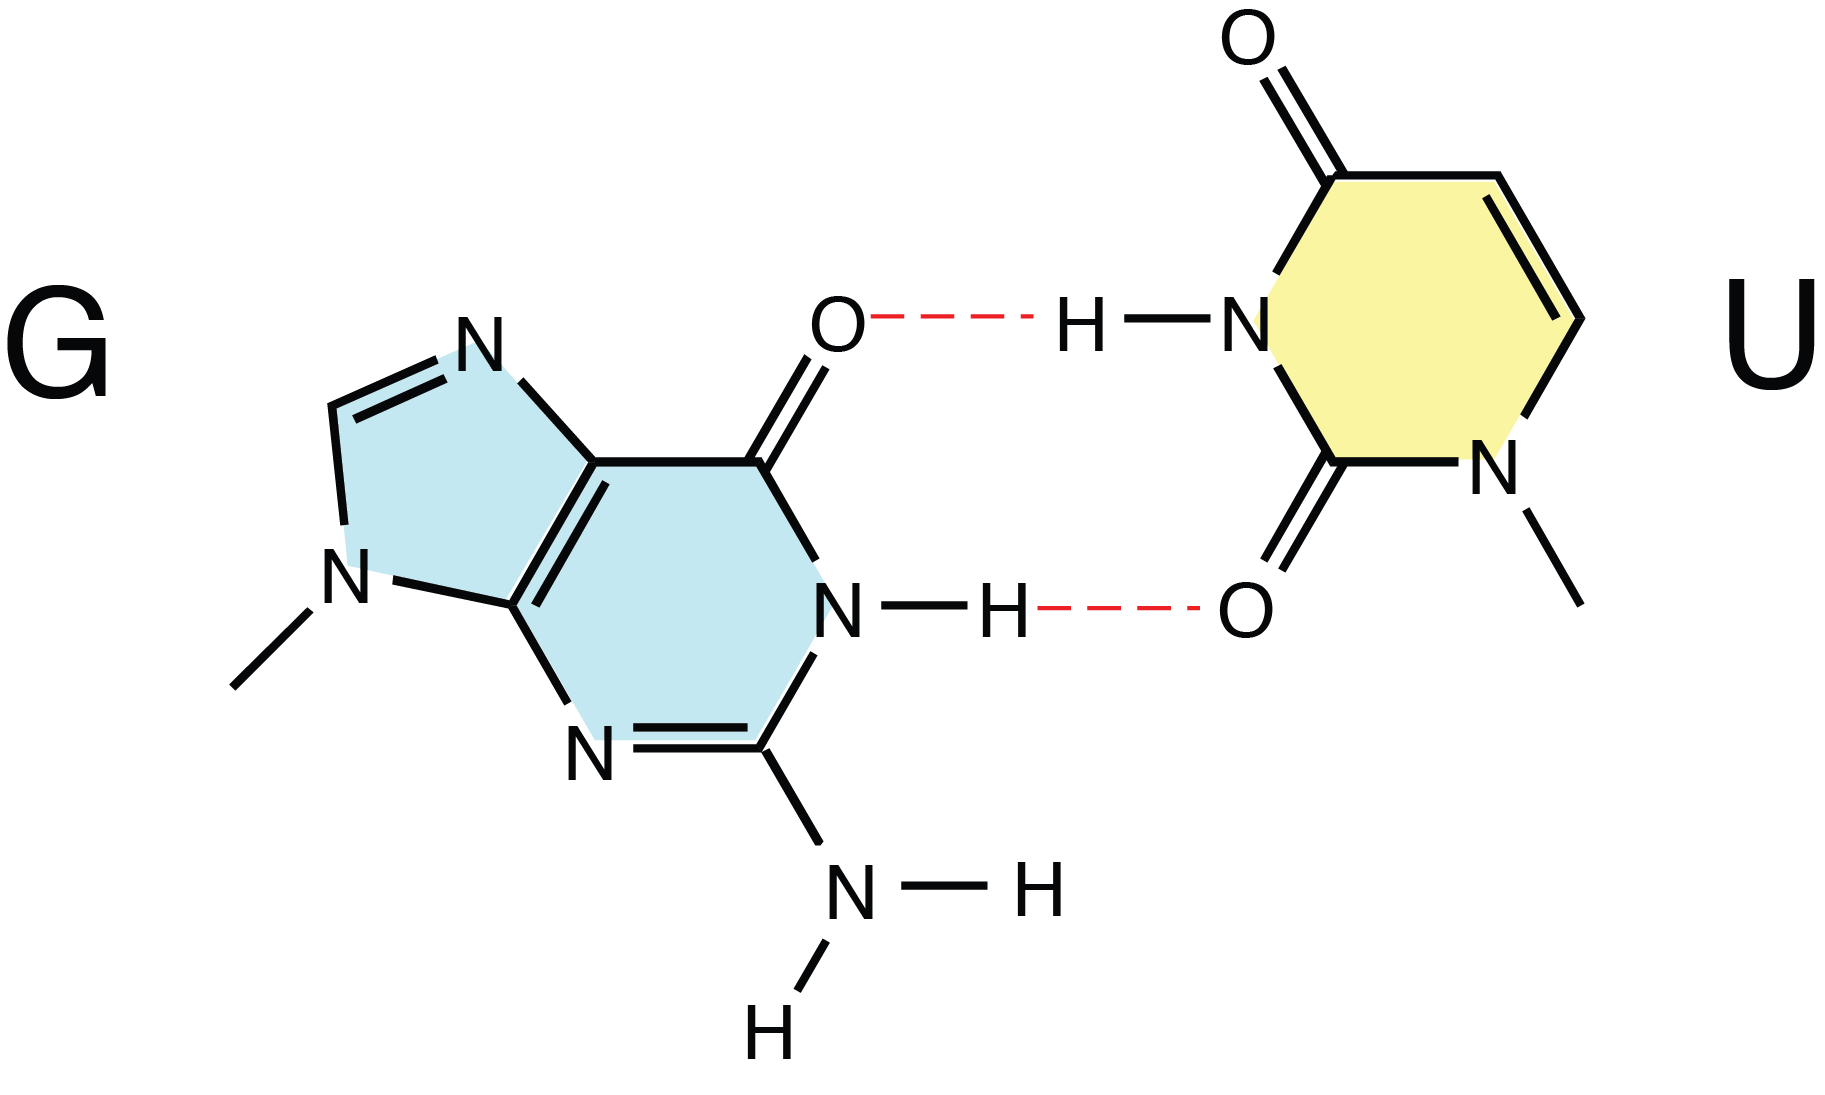
\includegraphics[width=0.3\textwidth]{fig03/rna_gu_wobble.png}
  \caption{GU wobble pairs \newline (modified  from the original version by \href{https://commons.wikimedia.org/w/index.php?curid=2636730}{Fdardel, Wikimedia Commons})}
\end{figure}

\noindent \textbf{Example of DP for RNA pairs} \\
\noindent You can form the following DP table for two RNA sequences: q = AU and d = UGA with gap penalty g = 9.
\begin{multicols}{2}
DP table:
\begin{figure}[H]
  \centering
      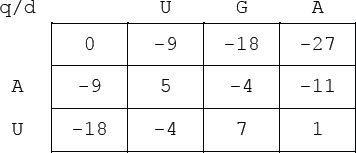
\includegraphics[width=0.25\textwidth]{fig03/example_rna_alignment.png}
\end{figure}

Alignment:
\begin{verbatim}
    q: A-U
    d: UGA
\end{verbatim}

\end{multicols} 

%
% Similarity of protein sequences
%
\subsubsection*{Similarity of protein sequences}
Amino acids can be categorized into several groups by their properties. Proteins alignments often need to take these properties into consideration.

\begin{figure}[H]
  \centering
      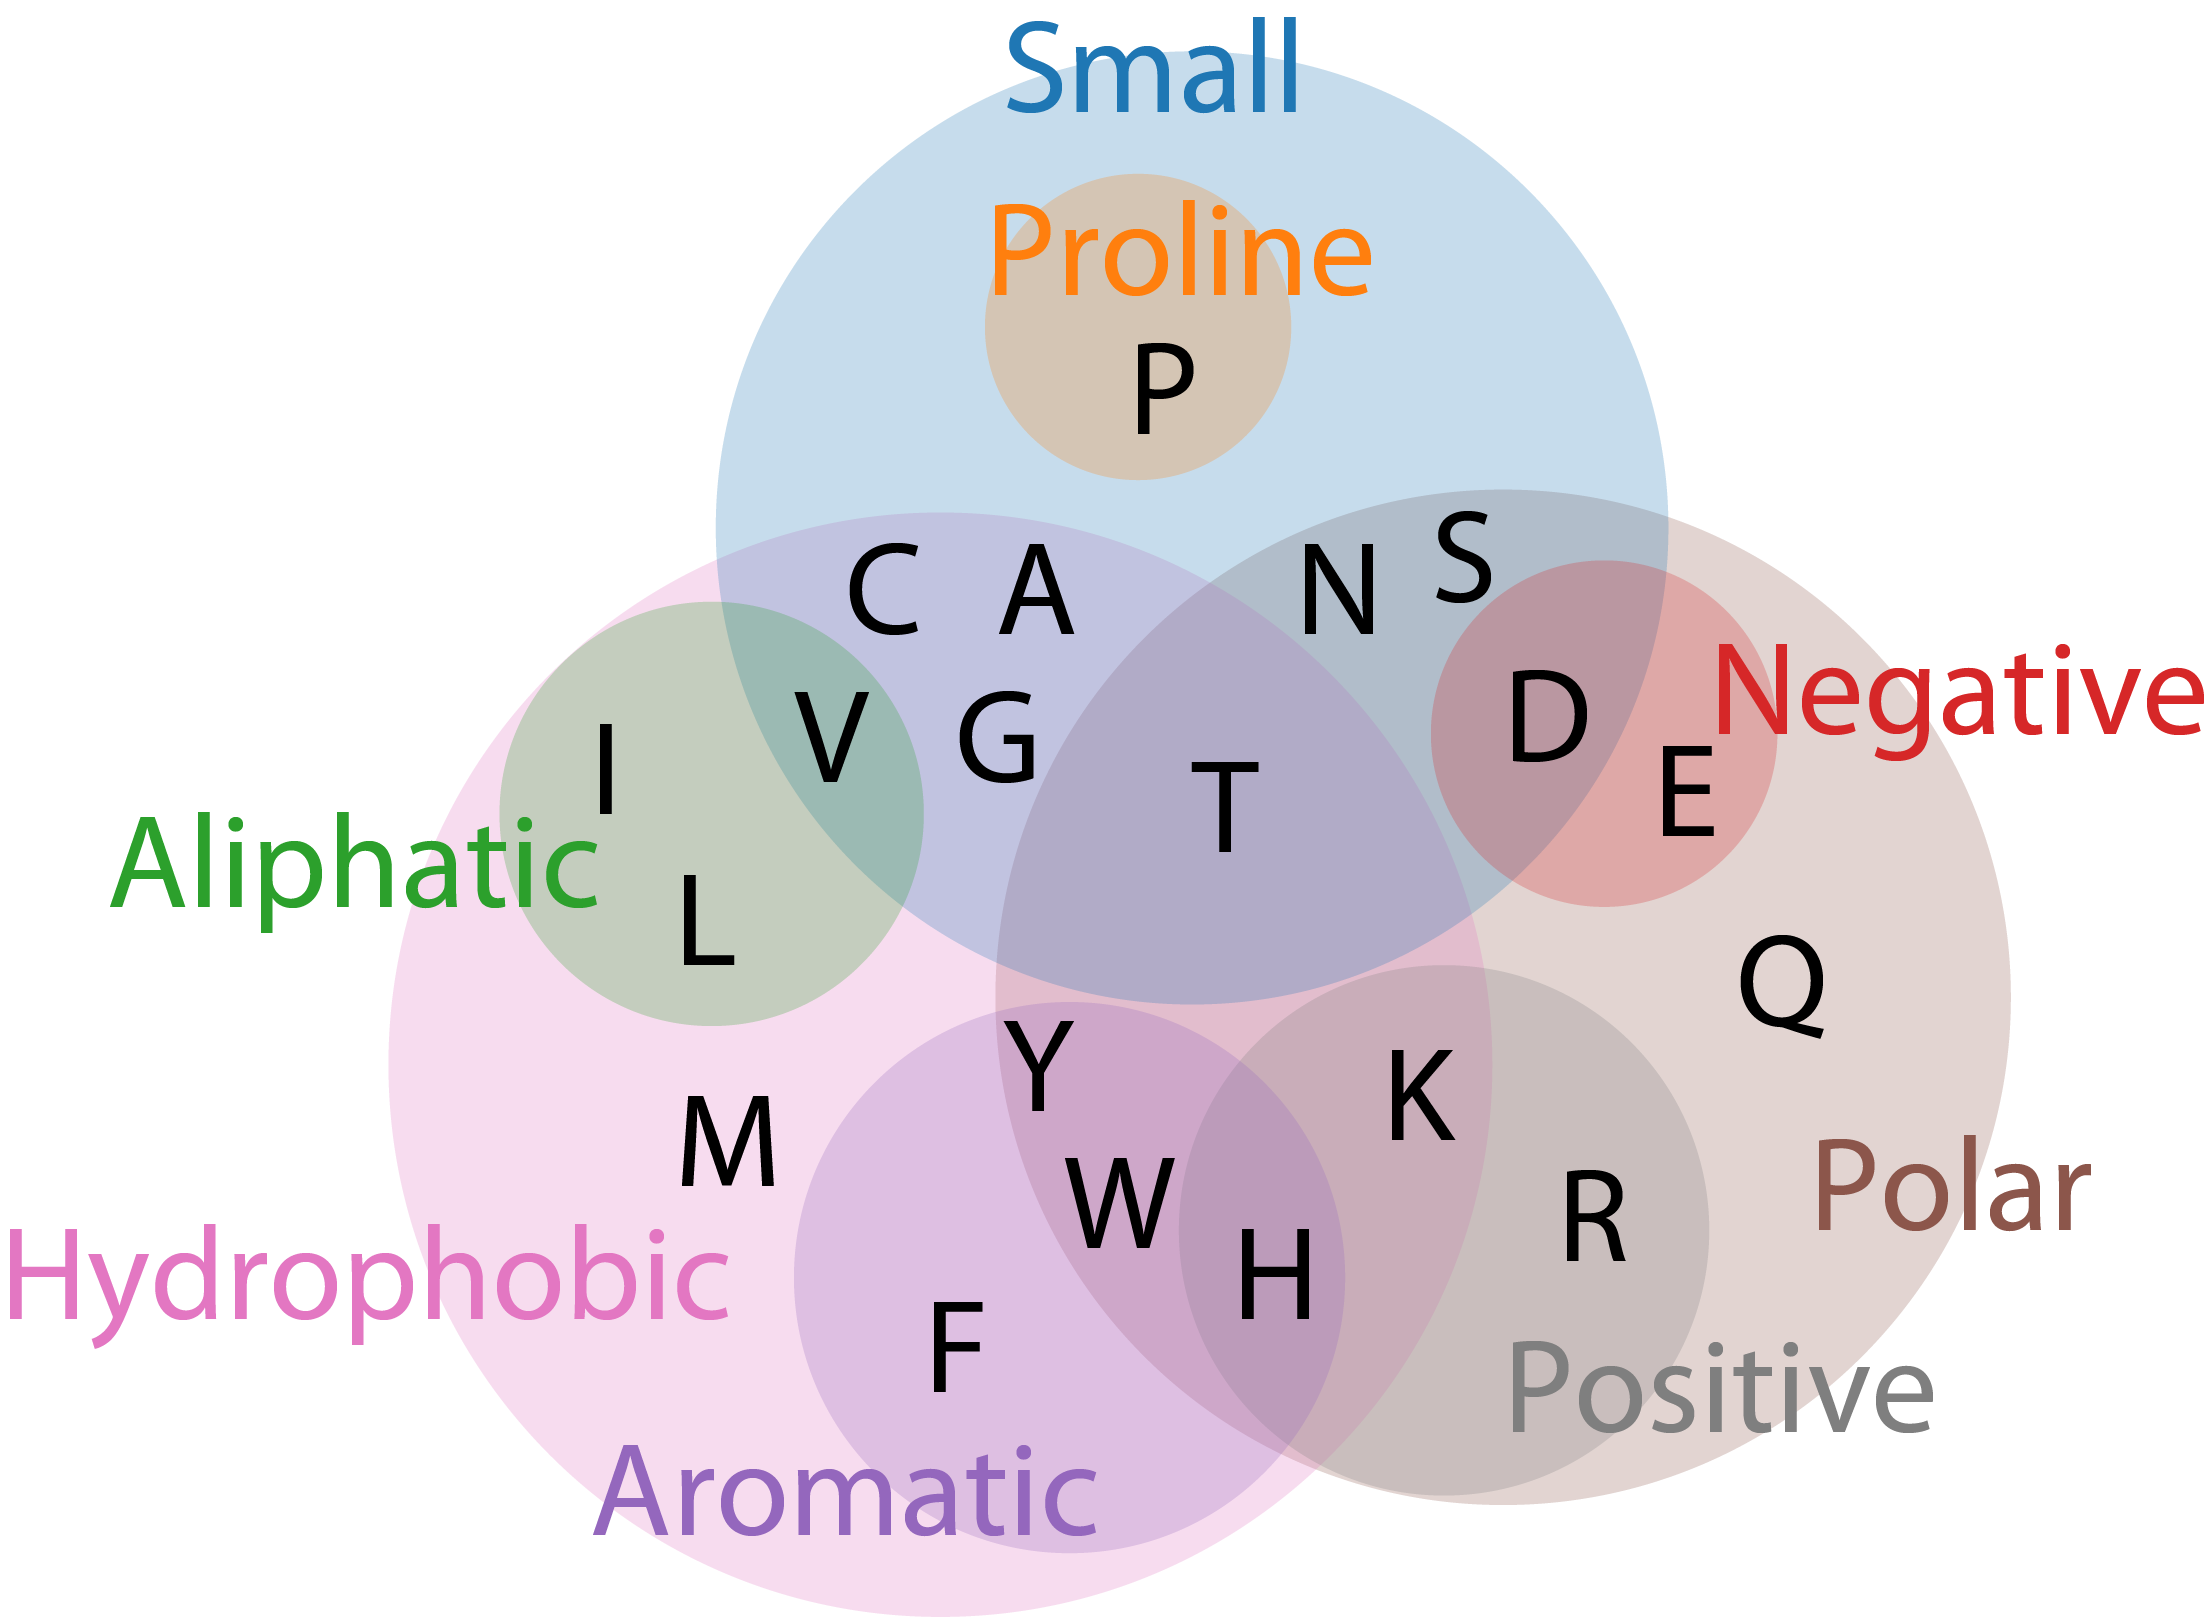
\includegraphics[width=0.3\textwidth]{fig03/amino_acid_properties.png}
  \caption{Venn diagram of amino acid properties }
\end{figure}

\noindent
\textbf{Example of a protein score matrix}\\
It can be used to compare the similarity between two protein sequences.

\begin{table}[!ht]
\footnotesize
\centering

\label{my-label}
\begin{tabular}{lllllllllllllllllllll}
   & \textbf{A }  & \textbf{R}   & \textbf{N}   & \textbf{D }  & \textbf{C}   & \textbf{Q}   & \textbf{E}   & \textbf{G}   & \textbf{H }  & \textbf{I}   & \textbf{L}   & \textbf{K}   & \textbf{M}   & \textbf{F}   & \textbf{P}   & \textbf{S}   & \textbf{T}   & \textbf{W}   & \textbf{Y}   & \textbf{V}   \\
\textbf{A} & 13  & 6   & 9   & 9   & 5   & 8   & 9   & 12  & 6   & 8   & 6   & 7   & 7   & 4   & 11  & 11  & 11  & 2   & 4   & 9   \\
\textbf{R} & 3   & 17  & 4   & 3   & 2   & 5   & 3   & 2   & 6   & 3   & 2   & 9   & 4   & 1   & 4   & 4   & 3   & 7   & 2   & 2   \\
\textbf{N} & 4   & 4   & 6   & 7   & 2   & 5   & 6   & 4   & 6   & 3   & 2   & 5   & 3   & 2   & 4   & 5   & 4   & 2   & 3   & 3   \\
\textbf{D} & 5   & 4   & 8   & 11  & 1   & 7   & 10  & 5   & 6   & 3   & 2   & 5   & 3   & 1   & 4   & 5   & 5   & 1   & 2   & 3   \\
\textbf{C} & 2   & 1   & 1   & 1   & 52  & 1   & 1   & 2   & 2   & 2   & 1   & 1   & 1   & 1   & 2   & 3   & 2   & 1   & 4   & 2   \\
\textbf{Q} & 3   & 5   & 5   & 6   & 1   & 10  & 7   & 3   & 7   & 2   & 3   & 5   & 3   & 1   & 4   & 3   & 3   & 1   & 2   & 3   \\
\textbf{E }& 5   & 4   & 7   & 11  & 1   & 9   & 12  & 5   & 6   & 3   & 2   & 5   & 3   & 1   & 4   & 5   & 5   & 1   & 2   & 3   \\
\textbf{G} & 12  & 5   & 10  & 10  & 4   & 7   & 9   & 27  & 5   & 5   & 4   & 6   & 5   & 3   & 8   & 11  & 9   & 2   & 3   & 7   \\
\textbf{H} & 2   & 5   & 5   & 4   & 2   & 7   & 4   & 2   & 15  & 2   & 2   & 3   & 2   & 2   & 3   & 3   & 2   & 2   & 3   & 2   \\
\textbf{I }& 3   & 2   & 2   & 2   & 2   & 2   & 2   & 2   & 2   & 10  & 6   & 2   & 6   & 5   & 2   & 3   & 4   & 1   & 3   & 9   \\
\textbf{L} & 6   & 4   & 4   & 3   & 2   & 6   & 4   & 3   & 5   & 15  & 34  & 4   & 20  & 13  & 5   & 4   & 6   & 6   & 7   & 13  \\
\textbf{K} & 6   & 18  & 10  & 8   & 2   & 10  & 8   & 5   & 8   & 5   & 4   & 24  & 9   & 2   & 6   & 8   & 8   & 4   & 3   & 5   \\
\textbf{M} & 1   & 1   & 1   & 1   & 0   & 1   & 1   & 1   & 1   & 2   & 3   & 2   & 6   & 2   & 1   & 1   & 1   & 1   & 1   & 2   \\
\textbf{F} & 2   & 1   & 2   & 1   & 1   & 1   & 1   & 1   & 3   & 5   & 6   & 1   & 4   & 32  & 1   & 2   & 2   & 4   & 20  & 3   \\
\textbf{P} & 7   & 5   & 5   & 4   & 3   & 5   & 4   & 5   & 5   & 3   & 3   & 4   & 3   & 2   & 20  & 6   & 5   & 1   & 2   & 4   \\
\textbf{S} & 9   & 6   & 8   & 7   & 7   & 6   & 7   & 9   & 6   & 5   & 4   & 7   & 5   & 3   & 9   & 10  & 9   & 4   & 4   & 6   \\
\textbf{T} & 8   & 5   & 6   & 6   & 4   & 5   & 5   & 6   & 4   & 6   & 4   & 6   & 5   & 3   & 6   & 8   & 11  & 2   & 3   & 6   \\
\textbf{W} & 0   & 2   & 0   & 0   & 0   & 0   & 0   & 0   & 1   & 0   & 1   & 0   & 0   & 1   & 0   & 1   & 0   & 55  & 1   & 0   \\
\textbf{Y} & 1   & 1   & 2   & 1   & 3   & 1   & 1   & 1   & 3   & 2   & 2   & 1   & 2   & 15  & 1   & 2   & 2   & 3   & 31  & 2   \\
\textbf{V} & 7   & 4   & 4   & 4   & 4   & 4   & 4   & 4   & 5   & 4   & 15  & 10  & 4   & 10  & 5   & 5   & 5   & 72  & 4   & 17 
\end{tabular}
\caption{Mutation probability matrix for the evolutionary distance of 250 PAMs (in percentage) (Chapter 22: A model of evolutionary change in proteins, Dayhoff and Schwartz, Atlas of Protein Sequence and Structure, 1978)}
\end{table}

%
% Exercise \thesection.1
%
\subsubsection*{Exercise \thesection.1}
\begin{enumerate}
\item Use the DNA score matrix below with g = 10 and find the optimal alignment for q = TG and d = TCG.

\begin{figure}[H]
  \centering
      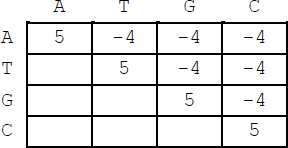
\includegraphics[width=0.25\textwidth]{fig03/dna_matrix_exercise.png}
\end{figure}

\item The 250 PAM mutation matrix above can not directly be used for global alignments. Explain what kind of matrix you need for calculating  alignment scores.
\end{enumerate}

\bigskip 

%\end{document}

%\documentclass[12pt]{article}
%\usepackage[a4paper, margin=1in]{geometry} 
%\usepackage{graphicx} 
%\usepackage{hyperref}
%\usepackage{float}
%\usepackage{multicol}
%\usepackage[font=small, labelfont=bf]{caption}
%
%\begin{document}

%
% Extension of gap penalties
%
\subsection{Extension of gap penalties}

%
% Types of gap penalties
%
\subsubsection*{Types of gap penalties}
Three types of gap penalties can be considered when creating an alignment. They treat a gap penalty differently depending on the gap length.

\begin{itemize}
\item Linear
\item Affine
\item Constant
\end{itemize}

%
% Gap penalty notation
%
\subsubsection*{Gap penalty notation}
\begin{itemize}
\item $g$: single gap penalty
\item $l$: length of a gap
\item $g_l$: gap penalty of length l
\item $g_{open}$: initial gap penalty
\item $g_{extend}$: extended gap penalty
\end{itemize}

%
% Linear gap penalty
%
\subsubsection*{Linear gap penalty}
It is the same as our simple scoring scheme. It treats a gap with multiple blanks as a result of several mutations. A gap of length $l$ can be calculated as: $g_l = g * l$.
\medskip 

\noindent
\textbf{Example of a gap of length 2}
\begin{verbatim}
    q: ACCCGT
    d: AC--GT
\end{verbatim}
The score of the gap (only the gap part) is 10 when $g$ = 5. 

%
% Affine gap penalty
%
\subsubsection*{Affine gap penalty}
It treats a gap with multiple blanks as a result of a single mutation. A gap with length $l$ can be calculated as: $g_l = g_{open} + (l – 1) * g_{extend}$.
\medskip 

\noindent
\textbf{Example of a gap of length 2}
\begin{verbatim}
    q: ACCCGT
    d: AC--GT
\end{verbatim}
The score of the gap (only the gap part) is 5.5 when $g_{open}$ and $g_{extend}$ are 5 and 0.5 respectively. 

%
% Constant gap penalty
%
\subsubsection*{Constant gap penalty}
It is similar to the affine gap penalty, but the score is independent form the gap length. A gap with length l can be calculated as: $g_l = g$ 
\medskip 

\noindent
\textbf{Example of a gap of length 2}
\begin{verbatim}
    q: ACCCGT
    d: AC--GT
\end{verbatim}
The score of the gap (only the gap part) for the alignment above is 5 when $g$ = 5. 

%
% Exercise \thesection.2
%
\subsubsection*{Exercise \thesection.2}
Calculate all three types of gap penalties for the gap in alignment 1 \& 2.

\begin{itemize}
\item $g$: 5
\item $g_{open}$: 5
\item $g_{extend}$: 0.5
\end{itemize}

\begin{multicols}{2}
\begin{verbatim}
Alignment 1
    q: CCCGG 
    d: CC-CG
\end{verbatim}

\begin{verbatim}
Alignment 2 
    q: CCCGG
    d: C---G
\end{verbatim}
\end{multicols}

%\end{document}

%\documentclass[12pt]{article}
%\usepackage[a4paper, margin=1in]{geometry} 
%\usepackage{graphicx} 
%\usepackage{hyperref}
%\usepackage{float}
%\usepackage{multicol}
%\usepackage{amsmath}
%\usepackage[font=small, labelfont=bf]{caption}
%
%\begin{document}

%
% Affine gap penalties with a single DP table
%
\subsection{Affine gap penalties with a single DP table}

%
% DP for general gap penalty
%
\subsubsection*{DP for general gap penalty}
We need to modify DP so that extra cells are checked to find the optimal score of a cell. 

%
% Cell update rule of general gap penalty
%
\subsubsection*{Cell update rule of general gap penalty}
\null \medskip  
\begin{equation*}
H_{i,j} =\max \left[H_{i-1,j-1} + R_{q_{i}d_{j}}, \quad \max_{1 \leq l \leq j}(H_{i,j-l} - g_l) ,  \quad \max_{1 \leq l \leq i}(H_{i-l,j} - g_l) \right]
\end{equation*}

%
% NEWPAGE
%
\newpage

\noindent
\textbf{Example of cell update}

\begin{multicols}{2}
Sequences:
\begin{verbatim}
    q: AG, d: ACG
\end{verbatim}
\vfill\null
\columnbreak

\noindent
Scoring scheme: \\
\null \quad $g_{open}$ = 1 \\
\null \quad $g_{extend}$ = 0.1 \\
\null \quad $R_{ab}$ = 1 for a = b \\ 
\null \quad $R_{ab}$ = 0 for a $\neq$ b \\ 

\end{multicols} 

\textbf{Update $H_{2,1}$}

\begin{figure}[H]
  \centering
      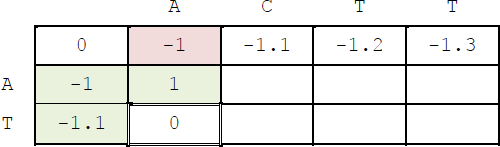
\includegraphics[width=0.5\textwidth]{fig03/dp_general_gap_example_1.png}
\end{figure}

\begin{itemize}
\item vertical:   $max(1 - 1, \quad -1 - 1 - 0.1) = 0$
\item horizontal: $-1.1 - 1 = -2.1$
\item diagonal: $-1 - 0 = -1$
\end{itemize}

\null \medskip 
\textbf{Update $H_{1,2}$}

\begin{figure}[H]
  \centering
      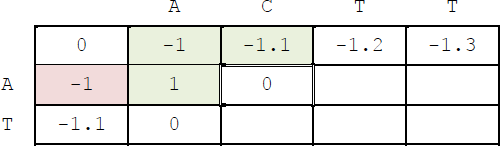
\includegraphics[width=0.5\textwidth]{fig03/dp_general_gap_example_2.png}
\end{figure}

\begin{itemize}
\item vertical: $-1.1 - 1 = -2.1$
\item horizontal: $max(1 - 1, \quad -1 - 1 - 0.1) = 0$
\item diagonal: $-1 - 0 = -1$
\end{itemize}

\null \medskip 
\textbf{Update $H_{1,3}$}

\begin{figure}[H]
  \centering
      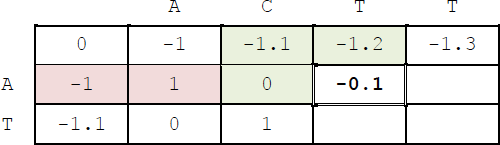
\includegraphics[width=0.5\textwidth]{fig03/dp_general_gap_example_3.png}
\end{figure}

\begin{itemize}
\item vertical: $-1.2 - 1 = -2.2$
\item horizontal: $max(0 - 1, \quad 1 - 1 - 0.1, \quad  -1 -1 - 0.1 - 0.1) = -0.1$
\item diagonal: $-1.1 - 0 = -1.1$
\end{itemize}


%
% Exercise \thesection.3
%
\subsubsection*{Exercise \thesection.3}
Complete the DP table below.

\begin{multicols}{2}
Sequences:
\begin{verbatim}
    q: AT, d: ACTT
\end{verbatim}
\vfill\null
\columnbreak

\noindent
Scoring scheme: \\
\null \quad $g_{open}$ = 1 \\
\null \quad $g_{extend}$ = 0.1 \\
\null \quad $R_{ab}$ = 1 for a = b \\ 
\null \quad $R_{ab}$ = 0 for a $\neq$ b \\ 

\end{multicols} 

\begin{figure}[H]
  \centering
      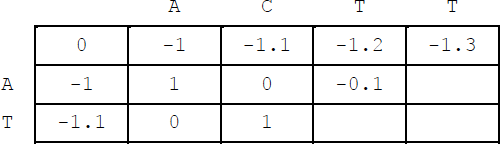
\includegraphics[width=0.5\textwidth]{fig03/dp_general_gap_exercise.png}
\end{figure}

%\end{document}

%\documentclass[12pt]{article}
%\usepackage[a4paper, margin=1in]{geometry} 
%\usepackage{graphicx} 
%\usepackage{hyperref}
%\usepackage{float}
%\usepackage{multicol}
%\usepackage{amsmath}
%\usepackage[font=small, labelfont=bf]{caption}
%
%\begin{document}

%
% Affine gap penalties with three DP tables
%
\subsection{Affine gap penalties with three DP tables}
DP can effectively solve affine gap penalties with three tables.

\begin{figure}[H]
  \centering
      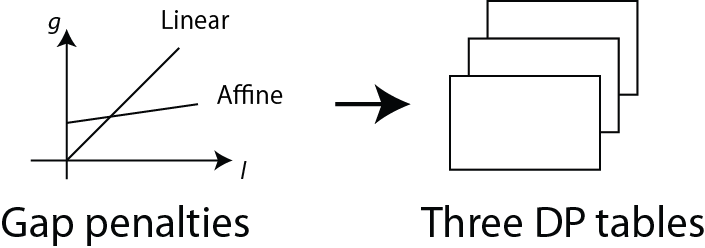
\includegraphics[width=0.4\textwidth]{fig03/three_dp_tables_for_affine.png}
  \caption{Affine gap penalties and three tables}
\end{figure}

%
% Three DP tables
%
\subsubsection*{Three DP tables}
We need to modify DP so that extra cells are checked to find the optimal score of a cell. 

\begin{itemize}
\item $E_{i,j}$: alignment ending with a gap extend (vertical)
\item $F_{i,j}$: alignment ending with a gap extend (horizontal)
\item $G_{i,j}$: alignment ending with a match/mismatch (diagonal)
\end{itemize}

%
% Cell update rule of the three tables
%
\subsubsection*{Cell update rule of the three tables}

\begin{align*}
E_{i,j} &= max(E_{i-1,j} - g_{extend}, \quad F_{i-1,j} - g_{open}, \quad G_{i-1,j} - g_{open}) \\
F_{i,j} &= max(E_{i,j-1} - g_{open}, \quad F_{i,j-1} - g_{extend}, \quad G_{i,j-1} - g_{open}) \\
G_{i,j} &= max(E_{i-1,j-1} + R_{q_{i}d_{j}}, \quad F_{i-1,j-1}+ R_{q_{i}d_{j}}, \quad G_{i-1,j-1} + R_{q_{i}d_{j}})
\end{align*}

\noindent You can calculate H only in the last cell.
\begin{align*}
H_{m,n} = max(E_{m,n}, F_{m,n}, G_{m,n})
\end{align*}

\begin{figure}[H]
  \centering
      \includegraphics[width=0.25\textwidth]{fig03/three_dp_tables_update_for_affine.png}
  \caption{Update a cell with E, F, and G}
\end{figure}

%
% NEWPAGE
%
%\newpage

%
% Recurrence rules when i = 0 and j = 0
%
\subsubsection*{Recurrence rules when i = 0 and j = 0}
\begin{figure}[H]
  \centering
      \includegraphics[width=0.75\textwidth]{fig03/affine_dp_special_cases.png}
\end{figure}
\null \medskip 

%
% Example of updating DP tables with affine gaps
%
\subsubsection*{Example of updating DP tables with affine gaps}
\begin{multicols}{2}
Sequences:
\begin{verbatim}
    q: AT, d: ACTT
\end{verbatim}
\vfill\null
\columnbreak

\noindent
Scoring scheme: \\
\null \quad $g_{open}$ = 1 \\
\null \quad $g_{extend}$ = 0.1 \\
\null \quad $R_{ab}$ = 1 for a = b \\ 
\null \quad $R_{ab}$ = 0 for a $\neq$ b \\ 

\end{multicols} 
 
\textbf{Initialization}
\begin{figure}[H]
  \centering
      \includegraphics[width=0.75\textwidth]{fig03/affine_dp_init.png}
\end{figure}
\null \medskip 

\textbf{Update the first row}
\begin{figure}[H]
  \centering
      \includegraphics[width=0.75\textwidth]{fig03/affine_dp_first_row.png}
\end{figure}
\null \medskip 

\textbf{Update the second row}
\begin{figure}[H]
  \centering
      \includegraphics[width=0.75\textwidth]{fig03/affine_dp_update_h.png}
\end{figure}
\null \medskip 

\textbf{Update H}
\begin{figure}[H]
  \centering
      \includegraphics[width=0.75\textwidth]{fig03/affine_dp_backtrack.png}
\end{figure}
\null \medskip 

\textbf{Backtrack}
\begin{figure}[H]
  \centering
      \includegraphics[width=0.75\textwidth]{fig03/affine_dp_backtrack.png}
\end{figure}
\null \medskip 

\textbf{Optimal alignment}
\begin{verbatim}
    q: A--T    Score: 0.9
    d: ACTT
\end{verbatim}

%
% Constant gap penalty
%
\subsubsection*{Constant gap penalty}
DP with constant gap penalty can be solved in the same way as the affine gap penalty.
\begin{figure}[H]
  \centering
      \includegraphics[width=0.25\textwidth]{fig03/gap_penalty_constant.png}
  \caption{Constant gap penalty}
\end{figure}

%\end{document}


%\documentclass[12pt]{article}
%\usepackage[a4paper, margin=1in]{geometry} 
%\usepackage{graphicx} 
%\usepackage{hyperref}
%\usepackage{float}
%\usepackage{multicol}
%\usepackage{amsmath}
%\usepackage[font=small, labelfont=bf]{caption}
%
%\begin{document}

%
% Sequence distance
%
\subsection{Sequence distance}
Distances can be also used to indicate the similarity of an alignment.

%
% Edit distance
%
\subsubsection*{Edit distance}
The Levenshtein distance is one of the most commonly used edit distances in computer science.
\begin{align*}
\mathrm{Insertion}: & \quad AC  \rightarrow AGC  & (\varepsilon  \rightarrow G) \\
\mathrm{Deletion}: & \quad ATC \rightarrow AC & (T \rightarrow \varepsilon) \\
\mathrm{Substitution}: & \quad AAA \rightarrow ATA &  (A \rightarrow T) 
\end{align*}

%
% Scoring scheme for Levenshtein distance
%
\subsubsection*{Scoring scheme for Levenshtein distance}
\begin{itemize}
\item $R_{ab}$ = 0 for a = b
\item $R_{ab}$ = -1 for a $\neq$ b
\item g = 1
\end{itemize}

%
% Distance from DP score
%
\subsubsection*{Distance from DP score}
Given the best score $T$ from DP, the edit distance $d$ is $-T$.
\bigskip  

\noindent
\textbf{Example of edit distance with DP}
\begin{multicols}{2}
\begin{figure}[H]
  \centering
      \includegraphics[width=0.4\textwidth]{fig03/dp_for_edit_distance.png}
\end{figure}
\vfill\null
\columnbreak

\vfill\null
\noindent $T = -1$ \\\\
\noindent $d = 1$

\end{multicols} 

%
% Metric space
%
\subsubsection*{Metric space}
The edit distance constitutes a metric space.
\begin{itemize}
\item $d_{xy} = 0$ for $x = y$ 
\item $d_{xy} > 0$ for $x \neq y$
\item $d_{xy} = d_{yx}$
\item $d_{xy} \leq d_{xz} + d_{zy}$ for any $z$ (the triangle inequality)
\end{itemize}

%
% Mutation and distance
%
\subsubsection*{Mutation and distance}
Mutations may occur several times on the same position.

\medskip 
\noindent
\textbf{Example of single mutations} \\

\noindent
$ACGT \rightarrow AGT \rightarrow ACT \rightarrow AGT \rightarrow AGCT$

\medskip 
\noindent
Four mutations have occurred, but the edit distance is 2.

%
% Mutation and distance
%
\subsubsection*{Distance per column}
It indicates the number of mutations per column (nucleotide/amino acid).

\bigskip 
$D = d / $(length of the longest sequence)

%
% Correction of distance
%
\subsubsection*{Correction of distance}
The distance can be adjusted. Below is a simple correction approach for protein sequences.

\bigskip 
$K=-\ln⁡(1-D-1/5 D^2 )$
\begin{figure}[H]
  \centering
      \includegraphics[width=0.3\textwidth]{fig03/adjust_distance.png}
      \caption{Correction of distance $D$}
\end{figure}

\medskip 
\noindent
\textbf{Example of distance correction} \\

$D = 0.5$

$K = -\ln⁡(1 - 0.5 - 1/5  \times 0.25 ) = -\ln(0.45) \approx 0.8⁡$

%\end{document}



\newpage

%
% Local alignment
%
\setcounter{figure}{0}
\setcounter{table}{0}
\section{Local alignment}
%\documentclass[12pt]{article}
%\usepackage[a4paper, margin=1in]{geometry} 
%\usepackage{graphicx} 
%\usepackage{hyperref}
%\usepackage{float}
%\usepackage{multicol}
%\usepackage[font=small, labelfont=bf]{caption}
%
%\begin{document}

%
% Local alignments
%
\subsection{Local alignments}
Local pairwise alignments are aligned pairs of sub--sequences that have centain level of similarities.

%
% Deiffrence between global and local alignments
%
\subsubsection*{Deiffrence between global and local alignments} 

\begin{figure}[H]
  \centering
      \includegraphics[width=0.75\textwidth]{fig04/global_and_local_alignments.png}
  \caption{Global and local alignments}
\end{figure}

%
% Elements of local alignment
%
\subsubsection*{Elements of local alignment}
\begin{itemize}
\item Segment: a substring of a sequence
\item Segment pair: a pair of segments
\item Local alignment: an alignment of a segment pair
\end{itemize}

%
% Alignment methods
%
\subsubsection*{Elements of local alignment}
\begin{itemize}
\item Dynamic programming (Smith--Waterman)
\item Dot matrix
\end{itemize}

%
% Applications
%
\subsubsection*{Applications}
\begin{itemize}
\item Sequence motifs
\item Conserved regions
\item Inverted repeats
\end{itemize}

\bigskip 

%\end{document}

%\documentclass[12pt]{article}
%\usepackage[a4paper, margin=1in]{geometry} 
%\usepackage{graphicx} 
%\usepackage{hyperref}
%\usepackage{float}
%\usepackage{multicol}
%\usepackage{amsmath}
%\usepackage[ruled]{algorithm2e}
%\usepackage{amssymb}
%\usepackage[font=small, labelfont=bf]{caption}
%
%\begin{document}

%
% Local alignment with DP
%
\subsection{Local alignment with DP}
Dynamic programming can be used to find local alignments.

%
% Requirements
%
\subsubsection*{Requirements}
\begin{itemize}
\item Find all local alignments between two sequences
\item Assign scores to all local alignments
\end{itemize}

%
% Modification of DP for local alignments
%
\subsubsection*{Modification of DP for local alignments}
\begin{itemize}
\item The minimum alignment score must be 0
\item Some entries of the score matrix should be negative
\item Backtracking also needs to be modified
\end{itemize}

%
% Update rule of DP cells
%
\subsubsection*{Update rule of DP cells}
\begin{align*}
H_{i,j}^{(0)} &= H_{i-1,j} - g &(vertical) \\
H_{i,j}^{(1)} &= H_{i,j-1} - g	&(horizontal) \\
H_{i,j}^{(2)} &= H_{i-1,j-1} + R_{a,b} &(diagonal) \\
H_{i,j}^{(2)} &= 0 &(minimum \, score)
\end{align*}

%
% Example of cell update
%
\subsubsection*{Example of cell update}
\begin{multicols}{2}
\begin{figure}[H]
  \centering
      \includegraphics[width=0.3\textwidth]{fig04/local_alignment_cell_update.png}
\end{figure}

\noindent Scoring scheme: \\ 
\null \quad Match: 0.5 \\ 
\null \quad Mismatch: -0.3 \\ 
\null \quad Gap penalty: 0.5

\end{multicols} 

\begin{align*}
H_{i,j}^{(0)} &=  -0.1 &\hfill &(vertical) \\
H_{i,j}^{(1)} &= -0.3 &\hfill &(horizontal) \\
H_{i,j}^{(2)} &= -0.2 &\hfill &(diagonal) \\
H_{i,j}^{(2)} &= 0 & \checkmark &(minimum \, score)
\end{align*}
\medskip 

%
% Backtracking 
%
\subsubsection*{Backtracking for local alignments}
It starts from the cells with the maximum score instead of the right bottom cell.

\begin{itemize}
\item Start cells: cells with the maximum score 
\item End cells: cells with 0
\end{itemize}

\noindent
\textbf{N.B.} the end cell with score 0 should not be included in the alignment.

%
% Example of backtracking
%
\subsubsection*{Example of backtracking}

\begin{figure}[H]
  \centering
      \includegraphics[width=0.7 \textwidth]{fig04/local_alignment_backtrack.png}
\end{figure}

\medskip 

%
% Pseudo-code of local alignment with DP
%
\subsubsection*{Pseudo-code of updating DP table for local alignment}
The cells in the first row and the first column are initialized with 0.

\begin{algorithm}[H]
  \SetKwInOut{HAB}{$\mathrm{H_{i,j}}$}
  \SetKwInOut{RAB}{$\mathrm{R_{a,b}}$}
  \SetKwInOut{G}{$\mathrm{g}$}
  \SetKwData{dRAB}{$\mathrm{R_{a,b}}$}
  \SetKwData{dG}{$\mathrm{g}$}
  
  \BlankLine
    
  \HAB{Dynamic programming table}
  \RAB{Match/mismatch scores}
  \G{Gap penalty}
  
  \BlankLine \BlankLine
  
  \tcp{Initialization}
  \For{$i \leftarrow 0$ \KwTo $m$}{
    $\mathrm{H_{i,0}}$ $\leftarrow$ $\mathbf{0} $\;
  }
  \For{$j \leftarrow 1$ \KwTo $n$}{
    $\mathrm{H_{0,j}}$ $\leftarrow$ $\mathbf{0} $\;
  }
  
  \BlankLine \BlankLine
    
  \tcp{Main loop for table update}
  \For{$i \leftarrow 1$ \KwTo $m$}{
    \For{$j \leftarrow 1$ \KwTo $n$}{
      $\mathrm{H_{i,j}}$ $\leftarrow$ $max(\mathrm{\mathbf{0}, H_{i-1,j}} - \dG, \mathrm{H_{i,j-1}} - \dG, \mathrm{H_{i-1,j-1}}$ + \dRAB)\;
    }
  }
  
  \SetAlgoRefName{\thesection.1}
  \caption{Update dynamic programming table for global alignment}

\end{algorithm}

%
% Exercise \thesection.1
%
\subsubsection*{Exercise \thesection.1}
	
Use DP to find a local alignment.

\begin{multicols}{2}
\begin{figure}[H]
  \centering
      \includegraphics[width=0.4\textwidth]{fig04/local_alignment_exercise.png}
\end{figure}

\noindent Scoring scheme: \\ 
\null \quad Match: 0.2 \\ 
\null \quad Mismatch: -0.2 \\ 
\null \quad Gap penalty: 0.2

\end{multicols} 

\bigskip 

%\end{document}

%\documentclass[12pt]{article}
%\usepackage[a4paper, margin=1in]{geometry} 
%\usepackage{graphicx} 
%\usepackage{hyperref}
%\usepackage{float}
%\usepackage{multicol}
%\usepackage{amsmath}
%\usepackage[ruled]{algorithm2e}
%\usepackage{amssymb}
%\usepackage[font=small, labelfont=bf]{caption}
%
%\begin{document}

%
% Dot matrix
%
\subsection{Dot matrix}
Using a dot matrix is an effective and easy way to find local similarities.

%
% Basic concept
%
\subsubsection*{Basic concept}
It uses an $m \times n$ binary matrix from two sequences.

\begin{itemize}
\item A dot: match
\item Empty: mismatch
\end{itemize}

%
% Example of dot matrix
%
\subsubsection*{Example of dot matrix}
\begin{verbatim}
    q: ACATTAG, d: CATTTAGG
\end{verbatim}

\begin{figure}[H]
  \centering
      \includegraphics[width=0.3\textwidth]{fig04/dot_matrix.png}
  \caption{Dot matrix of $7 \times 8$}
\end{figure}

\noindent
It is easy to find segment pairs with a dot matrix. Contiguous dots along diagonals indicate local alignments. It is also easy to find other similarities. For instance, contiguous dots along anti-diagonals indicate reversed substrings.

%
% Filtering of dot matrix
%
\subsubsection*{Filtering of dot matrix}
Dot matrices usually get noisy with too many dots.  Overlapping windows are usually applied to reduce the noise.

\bigskip 
\noindent
\textbf{Example of filtering}

\begin{figure}[H]
  \centering
      \includegraphics[width=0.3\textwidth]{fig04/dot_matrix_filtered.png}
  \caption{Filtered dot matrix with window size 3 and threshold 3.}
\end{figure}

%
% Exercise \thesection.2
%
\subsubsection*{Exercise \thesection.2}
Find local similarities between two DNA sequences, \verb|q: GATTACA| and \verb|d: GGATTTAC|.

\begin{enumerate}
\item Create a dot matrix for the two sequences.
\item Filter dots with overlapping windows size 3 and threshold 3.
\end{enumerate}

\bigskip 

%\end{document}


\newpage

%
% PART III
%
\part{}

%
% Database search
%
\setcounter{figure}{0}
\setcounter{table}{0}
\section{Database search}
%\documentclass[12pt]{article}
%\usepackage[a4paper, margin=1in]{geometry} 
%\usepackage{graphicx} 
%\usepackage{hyperref}
%\usepackage{float}
%\usepackage{multicol}
%\usepackage{multirow}
%\usepackage[font=small, labelfont=bf]{caption}
%
%\begin{document}

%
% Biological databases
%
 \subsection{Biological databases}
Biological databases contain biological information, mainly collected from molecular biology experiments, life science literature, and bioinformatics analyses.

%
% Categories of databases
%
\subsubsection*{Categories of databases} 
Annual \href{http://nar.oxfordjournals.org}{Nucleic Acids Research} database issue includes the following database categories.

\begin{itemize}
\item Nucleotide Sequence Databases
\item RNA sequence databases
\item Protein sequence databases
\item Structure Databases
\item Proteomics Resources
\item Human and other Vertebrate Genomes
\item Genomics Databases (non-vertebrate)
\item Plant databases
\item Human Genes and Diseases
\item Metabolic and Signaling Pathways
\item Immunological databases
\item ...
\end{itemize}

%
% GenBank
%
\subsubsection*{GenBank} 
\begin{itemize}
\item A comprehensive database of publicly available nucleotide sequences
\item Produced and maintained by NCBI (National Center for Biotechnology Information, URL: \href{http://www.ncbi.nlm.nih.gov}{http://www.ncbi.nlm.nih.gov})
\end{itemize}

\begin{figure}[H]
  \centering
      \includegraphics[width=0.6 \textwidth]{fig05/genebank_stat.png}
  \caption{Growth of GenBank and WGS (source: \href{http://www.ncbi.nlm.nih.gov/genbank/statistics}{NCBI})}
\end{figure}

%
% UniProt
%
\subsubsection*{UniProt} 
\begin{itemize}
\item A central repository of protein data from Swiss-Prot, TrEMBL, and PIR-PSD databases
\item Maintained by the UniProt consortium
\end{itemize}

%
% Sequence data 
%
\subsubsection*{Sequence data} 
\begin{itemize}
\item Identifier
\item Sequence
\end{itemize}

\noindent
\textbf{Data format of sequence data} \\
FASTA is the most popular format for sequence data.
\begin{figure}[H]
  \centering
      \includegraphics[width=\textwidth]{fig05/fasta.png}
\end{figure}

%
% Annotation data
%
\subsubsection*{Annotation data} 
Sequences databases usually contain annotations in addition to sequences. 

\begin{itemize}
\item Notes and descriptions of important regions and components
\item Meta data
\end{itemize}

\noindent
\textbf{Data format of annotation data} \\
Annotation data can be downloaded in many different formats. GFF is one of the popular file formats for storing genomic features.
\begin{figure}[H]
  \centering
      \includegraphics[width=\textwidth]{fig05/gff3.png}
\end{figure}

%
% Tools
%
\subsubsection*{Tools}
Many database tools are available for various purposes.
 
\noindent
\textbf{Search tools for sequence databases}
\begin{itemize}
\item BLAST at NCBI (\href{http://blast.ncbi.nlm.nih.gov/Blast.cgi}{http://blast.ncbi.nlm.nih.gov/Blast.cgi})
\item BLAT/BLAST at Ensembl (\href{http://www.ensembl.org/Multi/Tools/Blast}{http://www.ensembl.org/Multi/Tools/Blast})
\end{itemize}

\noindent
\textbf{Data browsing tools of annotation and sequence data}
\begin{itemize}
\item UCSC Genome Browser (\href{https://genome.ucsc.edu}{https://genome.ucsc.edu})
\item Ensemble Genome Browser (\href{http://www.ensembl.org}{http://www.ensembl.org})
\end{itemize}

\noindent
\textbf{Data download tools for annotation and sequence data}
\begin{itemize}
\item UCSC Table Browser (\href{http://genome.ucsc.edu/cgi-bin/hgTables}{http://genome.ucsc.edu/cgi-bin/hgTables})
\item Ensemble BioMart (\href{http://www.ensembl.org/biomart}{http://www.ensembl.org/biomart})
\end{itemize}

\noindent
\textbf{Tools for protein data}
\begin{itemize}
\item UniProt (\href{https://www.uniprot.org}{https://www.uniprot.org})
\end{itemize}

\bigskip 

%\end{document}

%\documentclass[12pt]{article}
%\usepackage[a4paper, margin=1in]{geometry} 
%\usepackage{graphicx} 
%\usepackage{hyperref}
%\usepackage{float}
%\usepackage{multicol}
%\usepackage{multirow}
%\usepackage[font=small, labelfont=bf]{caption}
%
%\begin{document}

%
% Search in sequence databases
%
\subsection{Search in sequence databases}
Since biological databases contain a large number of sequences, heuristics search methods are usually applied to database search.

%
% Aims of database search
%
\subsubsection*{Aims of searching in sequence databases} 
\begin{itemize}
\item Find homologies 
\item Find segments with important functionality
\end{itemize}

%
% Main procedures of sequence search
%
\subsubsection*{Main procedures of sequence search} 
\begin{itemize}
\item Perform local pairwise alignments
\item Evaluate the alignments statistically
\end{itemize}

%
% Estimated computational time for dynamic programming (DP)
%
\subsubsection*{Estimated computational time for dynamic programming (DP)} 
\begin{table}[h]
\centering
\caption{Estimated computational time of DP for the three cases 1ms, 10ms, and 1sec}
\begin{tabular}{|l|lll|}
\hline
\multirow{2}{*}{\textbf{Time of one alignment}} & \multicolumn{3}{c|}{\textbf{Database size}}                 \\ \cline{2-4} 
                                                & \textbf{1000} & \textbf{1,000,000} & \textbf{1,000,000,000} \\ \hline
\textbf{1 ms}                                   & 1 sec         & 16 min             & 2.6 h                  \\ 
\textbf{10 ms}                                  & 10 sec        & 2.6 h              & 11 days                \\ 
\textbf{1 sec}                                  & 16 min        & 11 days            & 31 years               \\ \hline
\end{tabular}
\end{table}

%
% Heuristic approach
%
\subsubsection*{Heuristic approach} 
\begin{itemize}
\item Need to search billions of entries
\item Tradeoff between accuracy/precision and speed
\item Use n-gram based search
\item BLAST (Basic Local Alignment Search Tool)
\item BLAT (BLAST-like alignment tool)
\end{itemize}

\bigskip 

%\end{document}

%\documentclass[12pt]{article}
%\usepackage[a4paper, margin=1in]{geometry} 
%\usepackage{graphicx} 
%\usepackage{hyperref}
%\usepackage{float}
%\usepackage{multicol}
%\usepackage{multirow}
%\usepackage[font=small, labelfont=bf]{caption}
%
%\begin{document} 

%
% BLAST
%
\subsection{BLAST}
BLAST (Basic Local Alignment Search Tool) is the most popular tool to find homologous sequences in large-scale sequence databases.

%
% Methods
%
\subsubsection*{Methods} 
\begin{itemize}
\item Generate n-grams from query sequence
\item Find n-gram hits in database
\item Expand n-gram hits to HSP
\item Increase HSP scores
\item Introducing gaps
\item Give the expect values (E-values) to HSPs
\end{itemize}

%
% N-gram hits to HSP
%
\subsubsection*{N-gram hits to HSP} 
\begin{itemize}
\item Connect multiple n-gram hits 
\item Increase HSP score
\end{itemize}

\begin{figure}[H]
  \centering
      \includegraphics[width=0.75\textwidth]{fig05/extend_hsps.png}
  \caption{N-gram hits to HSPs}
\end{figure}

%
% Increase HSP score
%
\subsubsection*{Increase HSP score} 
BLAST changes the length of HSP by shortening or extending in order to increase the score.

\noindent
\textbf{Example}
\begin{figure}[H]
  \centering
      \includegraphics[width=0.45\textwidth]{fig05/extension_process.png}
  \caption{HSP extension process (source: \href{https://commons.wikimedia.org/w/index.php?curid=32912508}{DISP, Wikimedia Commons})}
\end{figure}

%
% Introducing gaps
%
\subsubsection*{Introducing gaps} 
Banded dynamic programming is used to introduce gaps to an HSP.

\begin{figure}[H]
  \centering
      \includegraphics[width=0.25\textwidth]{fig05/banded_dp.png}
  \caption{Banded DP with the starting seed pair}
\end{figure}

%
% E-value
%
\subsubsection*{E-value} 
``The Expect value (E) is a parameter that describes the number of hits one can expect to see by chance when searching a database of a particular size'' \\ \\
-- BLAST Frequently Asked questions (\href{http://blast.ncbi.nlm.nih.gov}{http://blast.ncbi.nlm.nih.gov})

\bigskip 

%\end{document}

%\documentclass[12pt]{article}
%\usepackage[a4paper, margin=1in]{geometry} 
%\usepackage{graphicx} 
%\usepackage{hyperref}
%\usepackage{float}
%\usepackage{multicol}
%\usepackage{multirow}
%\usepackage[font=small, labelfont=bf]{caption}
%
%\begin{document} 

%
% N-gram based search
%
\subsection{N-gram based search}
Using n-grams is a useful method to find segment pairs.

%
% Equivalent or related concepts to n-gram
%
\subsubsection*{Equivalent or related concepts to n-gram} 
\begin{itemize}
\item q-gram
\item n-letter word
\item n-tuple
\item n-mer
\end{itemize}

%
% Create n-grams
%
\subsubsection*{Create n-grams} 
Decomposing a given sequence into n-letter words creates a list of n-grams.

\medskip 

\noindent
\textbf{Example}

\begin{verbatim}
    q: ACGATT 
    
    Word size: 2
        AC, CG, GA, AT, TT
        
    Word size: 3    
        ACG, CGA, GAT, ATT
        
\end{verbatim}

%
% Find segment pairs in database sequences
%
\subsubsection*{Find segment pairs in database sequences} 
N-grams can be used to find segment pairs.

\medskip

\noindent
\textbf{Example}

\begin{verbatim}
    q: ACGATT 
    2-gram: AC, CG, GA, AT, TT
    
    d1: CTAAG
    0 hit

    d2: CGTAT
    2 hits

    d3: ATAGA
    2 hits
\end{verbatim}

\bigskip 

%\end{document}

%\documentclass[12pt]{article}
%\usepackage[a4paper, margin=1in]{geometry} 
%\usepackage{graphicx} 
%\usepackage{hyperref}
%\usepackage{float}
%\usepackage{multicol}
%\usepackage{multirow}
%\usepackage[font=small, labelfont=bf]{caption}
%
%\begin{document} 

%
% Lookup table of matching n-grams
%
\subsection{Lookup table of matching n-grams}
A lookup table can be used for effectively finding n-gram matches.

%
% Terminology
%
\subsubsection*{Terminology} 
\begin{itemize}
\item Indices: positions in q
\item Matching n-grams: Possible matching n-grams by threshold score $T$
\end{itemize}

%
% Example of a creating lookup table
%
\subsubsection*{Example of a creating lookup table} 

\begin{multicols}{2}
\begin{verbatim}
    q: ACGTAC 
    2-gram: AC, CG, GT, TA, AC
    T: 3
\end{verbatim}
\vfill\null
\columnbreak

Score matrix:
\begin{figure}[H]
      \includegraphics[width=0.25\textwidth]{fig05/score_matrix.png}
\end{figure}

\end{multicols} 

\medskip  

%
% 1. Index of q
%
\subsubsection*{Step 1. Index of q} 
Add indices to all n-grams.

\begin{table}[h]
\small
\begin{tabular}{|l|l|}
\hline
\textbf{Index} & \textbf{N-gram} \\ \hline
1              & AC              \\ \hline
2              & CG              \\ \hline
3              & GT              \\ \hline
4              & TA              \\ \hline
5              & AC              \\ \hline
\end{tabular}
\end{table}


%
% 2. Scores of segment pairs and matching n-grams
%
\subsubsection*{Step 2. Scores of segment pairs and matching n-grams} 

Calculate scores between the first n-gram AC and all its matching n-grams.
\begin{table}[H]
\small
\begin{tabular}{|l|l|l|}
\hline
\textbf{N-gram} & \textbf{Matching n-gram} & \textbf{Score} \\ \hline
AC              & AA                       & $2+(-2)=0$       \\ \hline
AC              & AC                       & $2+2=4$          \\ \hline
AC              & AG                       & $2+(-2)=0$       \\ \hline
AC              & AT                       & $2+1=3$          \\ \hline
AC              & CA                       & $(-2)+(-2)=-4$   \\ \hline
AC              & CC                       & $(-2)+2=0$       \\ \hline
AC              & CG                       & $(-2)+(-2)=-4$   \\ \hline
AC              & CT                       & $(-2)+1=-1$      \\ \hline
AC              & GA                       & $1+(-2)=-1$      \\ \hline
AC              & GC                       & $1+2=3$          \\ \hline
AC              & GG                       & $1+(-2)=-1$      \\ \hline
AC              & GT                       & $1+1=2$          \\ \hline
AC              & TA                       & $(-2)+(-2)=-4$   \\ \hline
AC              & TC                       & $(-2)+2=0$       \\ \hline
AC              & TG                       & $(-2)+(-2)=-4$   \\ \hline
AC              & TT                       & $(-2)+1=-1$      \\ \hline
\end{tabular}
\end{table}

\noindent
Use threshold $T =3$.
\begin{table}[H]
\small
\begin{tabular}{|l|l|l|}
\hline
\textbf{N-gram} & \textbf{Matching n-grams} & \textbf{Scores} \\ \hline
AC              & AC, AT, GC                & 4, 3, 3         \\ \hline
\end{tabular}
\end{table}

\noindent
Repeat the same procedure for all n-grams of q and add their indices.
\begin{table}[H]
\small
\begin{tabular}{|l|l|l|l|}
\hline
\textbf{Index} & \textbf{N-gram} & \textbf{Matching n-grams} & \textbf{Scores} \\ \hline
1              & AC              & AC, AT, GC                & 4, 3, 3         \\ \hline
2              & CG              & CG, TG, CA                & 4, 3, 3         \\ \hline
3              & GT              & GT, AT, GC                & 4, 3, 3         \\ \hline
4              & TA              & TA, CA, TG                & 4, 3, 3         \\ \hline
5              & AC              & AC, GC, AT                & 4, 3, 3         \\ \hline
\end{tabular}
\end{table}

%
% 3. Lookup table of matching n-grams
%
\subsubsection*{Step 3. Lookup table of matching n-grams} 

Transform the table above to create a lookup table of matching n-grams.
\begin{table}[H]
\small
\begin{tabular}{|l|l|l|}
\hline
\textbf{Matching n-gram} & \textbf{Indices of q} & \textbf{Scores of segment pairs} \\ \hline
AC                       & 1, 5                  & 4, 4                             \\ \hline
GC                       & 1, 3, 5               & 3, 3, 3                          \\ \hline
AT                       & 1, 3, 5               & 3, 3, 3                          \\ \hline
CG                       & 2                     & 4                                \\ \hline
TG                       & 2, 4                  & 3, 3                             \\ \hline
CA                       & 2, 4                  & 3, 3                             \\ \hline
GT                       & 3                     & 4                                \\ \hline
TA                       & 4                     & 4                                \\ \hline
\end{tabular}
\end{table}

%
% 4. Search
%
\subsubsection*{Step 4. Search} 

\begin{verbatim}
    d1: AAAGTG 
    
    2 hits
    GT – index: 3, score: 4
    TG – index: (2, 4), score: (3, 3)
\end{verbatim}

%
% Exercise \thesection.1
%
\subsubsection*{Exercise \thesection.1}
Create a lookup table of 2-grams with the indices of q and the scores of segment pairs. Use the threshold $T$ and pre-calculated scores of 2-gram segment pairs.

\begin{verbatim}
    q: CATG
    T: 3
\end{verbatim}

\noindent
The table below shows pre-calculated scores of 2-gram segment pairs.
\begin{table}[H]
\small
\begin{tabular}{|l|l|l|l|}
\hline
\multirow{2}{*}{\textbf{Matching n-gram}} & \multicolumn{3}{c|}{\textbf{N-gram}}    \\ \cline{2-4} 
                                          & \textbf{CA} & \textbf{AT} & \textbf{TG} \\ \hline
AA                                        & 0           & 0           & -1          \\ \hline
AC                                        & -4          & 3           & -4          \\ \hline
AG                                        & -1          & 0           & 0           \\ \hline
AT                                        & -4          & 4           & -4          \\ \hline
CA                                        & 4           & -4          & 2           \\ \hline
CC                                        & 0           & -1          & -1          \\ \hline
CG                                        & 3           & -4          & 3           \\ \hline
CT                                        & 0           & 0           & -1          \\ \hline
GA                                        & 0           & -1          & -1          \\ \hline
GC                                        & -4          & 2           & -4          \\ \hline
GG                                        & -1          & -1          & 0           \\ \hline
GT                                        & 4           & 3           & -4          \\ \hline
TA                                        & 3           & -4          & 3           \\ \hline
TC                                        & -1          & -1          & 0           \\ \hline
TG                                        & 2           & -4          & 4           \\ \hline
TT                                        & -1          & 0           & 0           \\ \hline
\end{tabular}
\end{table}

\bigskip 

%\end{document}

%\documentclass[12pt]{article}
%\usepackage[a4paper, margin=1in]{geometry} 
%\usepackage{graphicx} 
%\usepackage{hyperref}
%\usepackage{float}
%\usepackage{multicol}
%\usepackage{multirow}
%\usepackage[font=small, labelfont=bf]{caption}
%
%\begin{document} 

%
% Finite-state machine with n-grams
%
\subsection{Finite-state machine with n-grams}
Finite-state machine enables efficient database search by expanding the basic n-gram based search.

%
% Number of potential matching n-grams
%
\subsubsection*{Number of potential matching n-grams} 
The number of potential n-grams increases by the alphabet size and the word size.

\medskip 

\noindent
\textbf{DNA} \\
C = \{A, C, G, T\} \\
Word size 2  $\rightarrow$ $4^2$ = 16 \\
Word size 3  $\rightarrow$ $4^3$ = 64 \\
Word size 12  $\rightarrow$ $4^{12}$ = 16,777,216 \\

\noindent
\textbf{Protein} \\
C = \{A, R, N, D, C, Q, E, G, H, I, L, L, M, F, P, S, T, W, Y, V\} \\
Word size 2  $\rightarrow$ $20^2$ = 400 \\
Word size 3  $\rightarrow$ $20^3$ = 8000

%
% Number of potential matching n-grams
%
\subsubsection*{Finite-state machine} 
A finite-state machine can be used to scan database sequences instead of using a lookup table. Finite-state machines are usually faster than lookup tables.

\begin{figure}[H]
  \centering
      \includegraphics[width=0.6\textwidth]{fig05/fsm_turnstile.png}
  \caption{Finite-state machine for coin-operated turnstile  \newline (sources: \href{https://commons.wikimedia.org/w/index.php?curid=20269475}{Chetvorno} and \href{https://commons.wikimedia.org/w/index.php?curid=8930080}{Sebasgui} via Wikimedia Commons)}
\end{figure}

%
% Example of creating a FSM
%
\subsubsection*{Example of creating a finite-state machine} 

\begin{verbatim}
    q: ACGTAC, Word size: 2, T: 3
\end{verbatim} 

Lookup table
\begin{table}[H]
\small
\begin{tabular}{|l|l|l|}
\hline
\textbf{Matching n-gram} & \textbf{Indices of q} & \textbf{Scores of segment pairs} \\ \hline
AC                       & 1, 5                  & 4, 4                             \\ \hline
GC                       & 1, 3, 5               & 3, 3, 3                          \\ \hline
AT                       & 1, 3, 5               & 3, 3, 3                          \\ \hline
CG                       & 2                     & 4                                \\ \hline
TG                       & 2, 4                  & 3, 3                             \\ \hline
CA                       & 2, 4                  & 3, 3                             \\ \hline
GT                       & 3                     & 4                                \\ \hline
TA                       & 4                     & 4                                \\ \hline
\end{tabular}
\end{table}


\begin{figure}[H]
  \centering
      \includegraphics[width=0.4\textwidth]{fig05/fsm_example.png}
  \caption{Finite-state machine to output the indices of 2-grams}
\end{figure}

\begin{verbatim}
    d1: AAAGTG 
    
    2 hits
    GT – index: 3
    TG – index: (2, 4)
\end{verbatim}

%
% Exercise \thesection.2
%
\subsubsection*{Exercise \thesection.2}
Create a finite-state machine and use it to find a segment pair.


\begin{enumerate}
\item Create a finite-state machine for the lookup table for q: ACGTAC. Add both indices and scores to the edges.

\medskip 
Lookup table
\begin{table}[H]
\centering
\small
\begin{tabular}{|l|l|l|}
\hline
\textbf{Matching n-gram} & \textbf{Indices of q} & \textbf{Scores of segment pairs} \\ \hline
AC                       & 1, 5                  & 2, 2                             \\ \hline
CG                       & 2                     & 4                                \\ \hline
GT                       & 3                     & 2                                \\ \hline
TA                       & 4                     & 0                                \\ \hline
\end{tabular}
\end{table}

\item Use the finite-state machine and find a segment pair between q and d: AAAGTG.
\end{enumerate}

\bigskip 

%\end{document}


\newpage

%
% Evaluation of alignment scores
%
\setcounter{figure}{0}
\setcounter{table}{0}
\section{Evaluation of alignment scores}
%\documentclass[12pt]{article}
%\usepackage[a4paper, margin=1in]{geometry} 
%\usepackage{graphicx} 
%\usepackage{hyperref}
%\usepackage{float}
%\usepackage{multicol}
%\usepackage{multirow}
%\usepackage[font=small, labelfont=bf]{caption}
%
%\begin{document}

%
% Statistical analysis
%
\subsection{Statistical analysis}
Statistical tests are performed to give an explanation to observed alignment scores.

%
% Hypothesis testing
%
\subsubsection*{Hypothesis testing} 
\begin{itemize}
\item Alternative hypothesis
\item Null hypothesis
\end{itemize}

\begin{figure}[H]
  \centering
      \includegraphics[width=0.6 \textwidth]{fig06/hypotheses.png}
  \caption{The null hypothesis and the alternative hypothesis}
\end{figure}

%
% P-value
%
\subsubsection*{P-value} 
``The p-value is defined as the probability of obtaining a result equal to or more extreme than what was actually observed, assuming that the null hypothesis is true'' \\

\noindent
-- the p-value page on Wikipedia (\url{https://en.wikipedia.org/wiki/P-value})

%
% Significance level (\alpha)
%
\subsubsection*{Significance level ($\alpha$)} 
The significance level should be chosen to indicate strong/weak evidence against the null hypothesis. \\

\noindent
Significance levels 0.05 and 0.01 are often used in life sciences.
\begin{itemize}
\item Statistically significant: $\alpha$ = 0.05
\item Statistically highly significant: $\alpha$ = 0.01
\end{itemize}

%
% Common misunderstandings of p-value
%
\subsubsection*{Common misunderstandings of p-value} 
``The p-value is not the probability that the null hypothesis is true or the probability that the alternative hypothesis is false.'' \\

\noindent
-- the p-value page on Wikipedia (\url{https://en.wikipedia.org/wiki/P-value})

%
% Underlying (background) score distributions
%
\subsubsection*{Underlying (background) score distributions} 
\begin{table}[H]
\centering
\caption{Alignment methods and distributions}
\begin{tabular}{ll}
Method                     & Underlying distribution \\ \hline
Global alignment           & Unknown                 \\
Local alignment (ungapped) & Gumbel                 
\end{tabular}
\end{table}

\bigskip 

%\end{document}

%\documentclass[12pt]{article}
%\usepackage[a4paper, margin=1in]{geometry} 
%\usepackage{graphicx} 
%\usepackage{hyperref}
%\usepackage{float}
%\usepackage{multicol}
%\usepackage{multirow}
%\usepackage[font=small, labelfont=bf]{caption}
%
%\begin{document}

%
% Evaluation of global alignment
%
\subsection{Evaluation of global alignment}
The underlying distribution of global alignment scores is unknown.

%
% Random generation of sequences
%
\subsubsection*{Random generation of sequences} 
One needs to consider using the appropriate length and compositions of amino acids or nucleotides needs when creating randomised sequences. \\

\noindent
\textbf{Example}

\noindent
Input sequences
\begin{verbatim}
    q: ACGT
    d: AGTACC  
\end{verbatim}

\noindent
Frequencies: {$f_{A}$ = 0.2, $f_{C}$ = 0.4, $f_{G}$ = 0.1, $f_{T}$ = 0.3} \\
Length: 6

\begin{verbatim}
    d1: CCAGTC
    d2: TCACCG
    d3: CTTGAA
    ...
\end{verbatim}

%
% Frequency distributions
%
\subsubsection*{Frequency distributions} 
\begin{itemize}
\item Universal (e.g. the whole protein database)
\item Global (e.g. protein super families)
\item Local (e.g. query and database sequences)
\end{itemize}

%
% Additional constrains
%
\subsubsection*{Additional constrains} 
Constrains on sequences generation are often considered. 
\begin{itemize}
\item Di-amino acid frequencies
\item Sub-region specific frequencies
\end{itemize}

%
% Non-parametric test and p-value
%
\subsubsection*{Non-parametric test and p-value} 
The simplest non-parametric test is calculating the rank of the score for the original alignment as the p-value. \\

$p=(b+1)/(n+1)$ \\

\noindent
where $b$ is the number of randomly generated scores above the score of the original alignment, and $n$ is the sample size. \\ 

\noindent
\textbf{N.B.} $n$ should be sufficiently large (e.g. $>$1000) to estimate an accurate p-value. \\

% NEWPAGE
\newpage

\noindent
\textbf{Example}

\begin{figure}[H]
  \centering
      \includegraphics[width=0.5 \textwidth]{fig06/random_sequences.png}
  \caption{Randomly generated sequences and alignment scores}
\end{figure}

\begin{table}[H]
\centering
\tiny
\begin{tabular}{llllllllllllllllllll}
\hline
\multicolumn{1}{|l|}{1} & \multicolumn{1}{l|}{2}   & \multicolumn{1}{l|}{3}   & \multicolumn{1}{l|}{4}   & \multicolumn{1}{l|}{5}   & \multicolumn{1}{l|}{6}   & \multicolumn{1}{l|}{7}   & \multicolumn{1}{l|}{8}   & \multicolumn{1}{l|}{9}   & \multicolumn{1}{l|}{10}  & \multicolumn{1}{l|}{11}  & \multicolumn{1}{l|}{12} & \multicolumn{1}{l|}{13}  & \multicolumn{1}{l|}{14}  & \multicolumn{1}{l|}{15}  & \multicolumn{1}{l|}{16}  & \multicolumn{1}{l|}{17}  & \multicolumn{1}{l|}{18}  & \multicolumn{1}{l|}{19}  & \multicolumn{1}{l|}{20}  \\ \hline
\multicolumn{1}{|l|}{1} & \multicolumn{1}{l|}{1.1} & \multicolumn{1}{l|}{1.3} & \multicolumn{1}{l|}{1.4} & \multicolumn{1}{l|}{1.7} & \multicolumn{1}{l|}{2.1} & \multicolumn{1}{l|}{2.2} & \multicolumn{1}{l|}{2.2} & \multicolumn{1}{l|}{2.3} & \multicolumn{1}{l|}{2.5} & \multicolumn{1}{l|}{2.8} & \multicolumn{1}{l|}{3}  & \multicolumn{1}{l|}{3.2} & \multicolumn{1}{l|}{3.3} & \multicolumn{1}{l|}{3.4} & \multicolumn{1}{l|}{3.6} & \multicolumn{1}{l|}{4.2} & \multicolumn{1}{l|}{4.4} & \multicolumn{1}{l|}{4.7} & \multicolumn{1}{l|}{5.2} \\ \hline
                        &                          &                          &                          &                          &                          &                          &                          &                          &                          &                          &                         &                          &                          &                          &                          &                          & \multicolumn{2}{c}{\textbf{4.5}}                             &                         
\end{tabular}
\end{table}

p-value: $(2 + 1) / (20 + 1) = 0.1429$

\begin{itemize}
\item Significance level $\alpha = 0.2$:  reject the null hypothesis
\item Significance level $\alpha = 0.05$: the null hypothesis is not rejected
\end{itemize}

%
% Exercise \thesection.1
%
\subsubsection*{Exercise \thesection.1}

\begin{enumerate}
\item Calculate the frequencies of nucleotides from the four sequences below.

\begin{verbatim}
    d1: CCAGC
    d2: TCACG
    d3: CTTAA
    d4: AACAA
\end{verbatim}

Frequencies: \{$f_{A} = \quad$, $f_{C} = \quad$, $f_{G} =  \quad$, $f_{T} =  \quad$ \}

\item Calculate the p-value of the alignment below. 

\begin{verbatim}
    q: AACG
    d: A-CG
    Score: 40
\end{verbatim}

\noindent
Assume that the scores are pre-calculated for the alignments of the query sequence and nine randomly generated sequences as follows. Use them for the p-value calculation.

\begin{table}[H]
\centering
\small
\begin{tabular}{|l|l|l|l|l|l|l|l|l|l|}
\hline
\textbf{No.}   & 1 & 2  & 3  & 4  & 5  & 6  & 7  & 8  & 9  \\ \hline
\textbf{Score} & 4 & 14 & 33 & 45 & 74 & 76 & 82 & 83 & 94 \\ \hline
\end{tabular}
\end{table}


\end{enumerate}

\bigskip 

%\end{document}

%\documentclass[12pt]{article}
%\usepackage[a4paper, margin=1in]{geometry} 
%\usepackage{graphicx} 
%\usepackage{hyperref}
%\usepackage{float}
%\usepackage{multicol}
%\usepackage{multirow}
%\usepackage[font=small, labelfont=bf]{caption}
%\usepackage[table,xcdraw]{xcolor}
%
%\begin{document}

%
% Evaluation of local alignment
%
\subsection{Evaluation of local alignment}
The underlying distribution of local alignment scores is an extreme value distribution.

%
% Gumbel distribution
%
\subsubsection*{Gumbel distribution} 
The Gumbel distribution is a member of the extreme value distribution family. \\

\begin{figure}[H]
  \centering
      \includegraphics[width=0.4 \textwidth]{fig06/gumbel.png}
  \caption{Gumbel distribution (source: \href{https://commons.wikimedia.org/w/index.php?curid=4787663}{Herr blaschke, Wikimedia Commons})}
\end{figure}

\noindent
The cumulative distribution function (CDF) of the Gumbel distribution: \\
$F_Y(y) = exp⁡[-e^{-\lambda(y-\mu)}]$ \\

\noindent
Parameters
\begin{itemize}
\item $\mu$: the modal value of the distribution, characteristic value
\item $\lambda$: a measure of the variance, decay constant
\end{itemize}

%
% Extreme value distribution
%
\subsubsection*{Extreme value distribution}
An extreme value distribution is a limiting distribution for the minimum or the maximum of a sufficiently large sample. Ungapped alignments with large sequence lengths are known to have this type of distribution. \\

\noindent
\textbf{Example (m and n are not large in this example)}

\begin{table}[H]
\centering
\begin{tabular}{lllllllll}
                       &                        & A                        & C                                                & G                                              & C                        & A                        & C                                                & G                                              \\ \cline{2-9} 
\multicolumn{1}{l|}{}  & \multicolumn{1}{l|}{0} & \multicolumn{1}{l|}{0}   & \multicolumn{1}{l|}{0}                           & \multicolumn{1}{l|}{0}                         & \multicolumn{1}{l|}{0}   & \multicolumn{1}{l|}{0}   & \multicolumn{1}{l|}{0}                           & \multicolumn{1}{l|}{0}                         \\ \cline{2-9} 
\multicolumn{1}{l|}{C} & \multicolumn{1}{l|}{0} & \multicolumn{1}{l|}{0}   & \multicolumn{1}{l|}{\cellcolor[HTML]{FE0000}0.5} & \multicolumn{1}{l|}{0}                         & \multicolumn{1}{l|}{0.5} & \multicolumn{1}{l|}{0}   & \multicolumn{1}{l|}{\cellcolor[HTML]{FE0000}0.5} & \multicolumn{1}{l|}{0}                         \\ \cline{2-9} 
\multicolumn{1}{l|}{G} & \multicolumn{1}{l|}{0} & \multicolumn{1}{l|}{0}   & \multicolumn{1}{l|}{0}                           & \multicolumn{1}{l|}{\cellcolor[HTML]{FE0000}1} & \multicolumn{1}{l|}{0.5} & \multicolumn{1}{l|}{0.2} & \multicolumn{1}{l|}{0}                           & \multicolumn{1}{l|}{\cellcolor[HTML]{FE0000}1} \\ \cline{2-9} 
\multicolumn{1}{l|}{A} & \multicolumn{1}{l|}{0} & \multicolumn{1}{l|}{0.5} & \multicolumn{1}{l|}{0}                           & \multicolumn{1}{l|}{0.5}                       & \multicolumn{1}{l|}{0.7} & \multicolumn{1}{l|}{0.2} & \multicolumn{1}{l|}{0}                           & \multicolumn{1}{l|}{0.5}                       \\ \cline{2-9} 
\end{tabular}
\end{table}

\begin{table}[H]
\centering
\begin{tabular}{
>{\columncolor[HTML]{FE0000}}l |
>{\columncolor[HTML]{FE0000}}l |l|l|l|l|l}
CG & CG & GC  &     & AC   &     &     \\
CG & CG & GA  & ... & CG   & ... & ... \\ \hline
1  & 1  & 0.2 &     & -0.6 &     &    
\end{tabular}
\end{table}

%
% Parameter estimation
%
\subsubsection*{Parameter estimation}
The p-value of the Gumbel distribution can be calculated as: \\

$P[Y>y]=1-F_Y (y)=1-exp⁡[-e^{-\lambda(y-\mu)}]$ \\

\noindent
The parameters $\mu$ and $\lambda$ can be estimated from the arithmetic mean $m_{Y}$ and the variance $\sigma_{Y}^2$ of the observed sample. \\

$\lambda \approx 1.282 / \sigma_{Y}$ \\

$\mu \approx m_{Y} - 0.577/\lambda$

%
% Example of parameter estimation
%
\subsubsection*{Example of parameter estimation}
Below is the optimal local alignment with the score between q:ACAGACTACTA and  d:TCAGACTGGGAACCE.

\begin{verbatim}
    CAGACT
    CAGACT
    Score: 6
\end{verbatim}

\noindent
The mean and the variance of the alignment scores are estimated as follows from randomly generated sequences. \\

$m_{Y}$: 1.7221 \\

$\sigma_{Y}$: 1.6025 \\

\noindent
Then, $\lambda$ and $\mu$ are estimated from $m_{Y}$ and $\sigma_{Y}$. \\

$\lambda \approx 1.282 / 1.6025 = 0.8$ \\

$\mu \approx 1.7221- 0.577/0.8 \approx 1$  \\

\noindent
The p-value is approximately 0.0181 when $\lambda = 0.8$ and $\mu = 1$ . The test result is statistically significant ($\alpha$= 0.05), and therefore, the null hypothesis is rejected. \\

\noindent
\textbf{Conclusion:} The query and the database sequences are homologous (p-value: 0.0181).

\bigskip 

%\end{document}

%\documentclass[12pt]{article}
%\usepackage[a4paper, margin=1in]{geometry} 
%\usepackage{graphicx} 
%\usepackage{hyperref}
%\usepackage{float}
%\usepackage{multicol}
%\usepackage{multirow}
%\usepackage[font=small, labelfont=bf]{caption}
%\usepackage[table,xcdraw]{xcolor}
%
%\begin{document}

%
% Evaluation of database search
%
\subsection{Evaluation of database search}
BLAST reports bit scores and e-values as search result. Bit score are calculated from raw scores, and e-values represent the expected numbers of database hits.

%
% Example of BLAST output
%
\subsubsection*{Example of BLAST output} 
\begin{itemize}
\item q: HSBGPG Human gene for bone gla protein (BGP)
\item d: osteocalcin [Felis catus]
\item Sequence ID: XP\_003999760.1
\end{itemize}

\begin{table}[H]
\centering
\begin{tabular}{lllll}
\textbf{Score} & \textbf{Expect} & \textbf{Identities} & \textbf{Positives} & \textbf{Gaps} \\ \hline
38.5 bits (88)  & 3.5             & 19/25 (76\%)         & 20/25 (80\%)        & 0/25 (0\%)    
\end{tabular}
\end{table}

\begin{verbatim}
      Query      677      TAFVSKQEGSEVVKRPRRYLYQWLG    751
                           AFVSKQEGSEVV+R RRYL   LG	
      Sbjct       36      AAFVSKQEGSEVVRRLRRYLAPGLG     60
\end{verbatim}

%
% Karlin-Altschul statistics
%
\subsubsection*{Karlin-Altschul statistics} 
\begin{itemize}
\item $\lambda$ is a scalar parameter for score matrix 
\item $K$ is a scalar parameter for search space size
\end{itemize}

BLAST pre-calculates both parameters in a search space independent manner.

%
% Example of Karlin-Altschul statistics
%
\subsubsection*{Example of Karlin-Altschul statistics} 
\begin{itemize}
\item Matrix: BLOSUM62
\item Lambda: 0.267
\item K: 0.041
\end{itemize}

%
%  Sequence databases
%
\subsubsection*{Sequence databases} 
The NCBI site provides several databases for BLAST search.
\begin{itemize}
\item Nucleotide collection (nr/nt)
\item Non-redundant protein sequences (nr)
\end{itemize}

%
%  Example of  database statitics
%
\subsubsection*{Example of  database statitics} 
\begin{itemize}
\item Database: nr
\item Number of letters: 41,667,927,126
\item Number of sequences: 113,671,629
\end{itemize}

\bigskip 

%\end{document}

%\documentclass[12pt]{article}
%\usepackage[a4paper, margin=1in]{geometry} 
%\usepackage{graphicx} 
%\usepackage{hyperref}
%\usepackage{float}
%\usepackage{multicol}
%\usepackage{multirow}
%\usepackage[font=small, labelfont=bf]{caption}
%\usepackage[table,xcdraw]{xcolor}
%\usepackage{amsmath}
%
%\begin{document}

%
% Bit score and e-value
%
\subsection{Bit score and e-value}
BLAST reports bit-scores and e-values that can be used for evaluation on search results.

%
% Bit score
%
\subsubsection*{Bit score} 
Bit scores are normalized scores that have the same unit (bit). The scores can be comparable even when different scoring schemes are used. \\

$S' = \dfrac{(\lambda S - ln⁡K)}{ln⁡2}$ \\

\noindent
$2^{S'}$ is the estimated number of alignments, and at least one alignment among them is estimated to have score S.

%
% Example of bit score calculation
%
\subsubsection*{Example of bit score calculation} 
\begin{itemize}
\item Lambda ($\lambda$): 0.267
\item K: 0.041
\item Score: 88
\end{itemize}

$S' = \dfrac{(\lambda S - ln⁡K)}{ln⁡2} = \dfrac{(0.267 * 88 -  ln⁡0.041)}{ln⁡2} = 38.506$\\

$2^{S'} = 2^{38.506} = 390,300,663,957$

%
% E-value
%
\subsubsection*{E-value} 
``The Expect value (E) is a parameter that describes the number of hits one can expect to see by chance when searching a database of a particular size'' \\ \\
-- BLAST Frequently Asked questions (\href{http://blast.ncbi.nlm.nih.gov}{http://blast.ncbi.nlm.nih.gov}) \\

$E(S) = Kmne^{-λS} = \dfrac{mn}{2^{S'}}$\\

%
% Example of E-value calculation
%
\subsubsection*{Example of E-value calculation} 
\begin{itemize}
\item n: 25
\item m: 41,667,927,126
\item Lambda ($\lambda$): 0.267
\item K: 0.041
\item Score: 88
\end{itemize}

$E(88) = Kmne^{-\lambda S} = \dfrac{41,667,927,126 \times 25}{2^{S'}} = 2.669$\\

%
% Exercise \thesection.2
%
\subsubsection*{Exercise \thesection.2}

\begin{itemize}
\item $\lambda$: 1.28
\item K: 0.5
\item m: 1000
\item n: 100
\end{itemize}

Calculate exp(-1.28) as 0.28.

\begin{enumerate}
\item What is the e-value of the score 1? 
\bigskip 
\item Is the alignment with score 1 likely homologous?
\end{enumerate}

\bigskip 

%\end{document}


\newpage

%
% Model evaluation
%
\setcounter{figure}{0}
\setcounter{table}{0}
\section{Model evaluation}
%\documentclass[12pt]{article}
%\usepackage[a4paper, margin=1in]{geometry} 
%\usepackage{graphicx} 
%\usepackage{hyperref}
%\usepackage{float}
%\usepackage{multicol}
%\usepackage{multirow}
%\usepackage[font=small, labelfont=bf]{caption}
%
%\begin{document}

%
% Evaluation of binary classifiers 
%
\subsection{Evaluation of binary classifiers}
Binary classifiers are mathematical or computational models that classify an input data set and produce the output with two labels. 

%
% Evaluation of models
%
\subsubsection*{Evaluation of models}
The performance of different models can be evaluated under the same test dataset.
\begin{itemize}
\item Algorithms
\item Scoring schemes
\item Statistical analysis
\end{itemize}

%
% Test data
%
\subsubsection*{Test data}
It should contain both homologous and non-homologous alignments.
\begin{itemize}
\item Positive: homologous
\item Negative: non-homologous
\end{itemize}

\begin{figure}[H]
  \centering
      \includegraphics[width=0.4 \textwidth]{fig07/test_data.png}
  \caption{Test dataset for homologous and non-homologous}
\end{figure}

%
% Model output
%
\subsubsection*{Model output} 
Different models often output different formats of scores. 

\begin{itemize}
\item Raw scores, bit scores, z-scores
\item P-values, e-values
\end{itemize}

\noindent
Threshold values are used to separate the result into positives and negatives.

\begin{figure}[H]
  \centering
      \includegraphics[width=0.4 \textwidth]{fig07/model_output.png}
  \caption{Model output for homologous and non-homologous}
\end{figure}

\bigskip 

%\end{document}

%\documentclass[12pt]{article}
%\usepackage[a4paper, margin=1in]{geometry} 
%\usepackage{graphicx} 
%\usepackage{hyperref}
%\usepackage{float}
%\usepackage{multicol}
%\usepackage{multirow}
%\usepackage[font=small, labelfont=bf]{caption}
%
%\begin{document}

%
% Confusion matrix 
%
\subsection{Confusion matrix}
The output of a model produces two false and two correct classifications. 

\begin{figure}[H]
  \centering
      \includegraphics[width=0.4 \textwidth]{fig07/four_outcomes.png}
  \caption{Four outcomes of model classification}
\end{figure}


%
% Example of model output
%
\subsubsection*{Example of model output}
A test dataset contains 10 positives and 10 negative. 

\begin{figure}[H]
  \centering
      \includegraphics[width=0.2 \textwidth]{fig07/example_model_output.png}
  \caption{An example of the four outcomes}
\end{figure}

\begin{itemize}
\item 7 true positives
\item 8 true negatives
\item 2 false positives
\item 3 false negatives
\end{itemize}

%
% Confusion matrix
%
\subsubsection*{Confusion matrix}
The classification result can be formed into a matrix format.

\begin{table}[H]
\centering
\caption{Confusion matrix}
\begin{tabular}{ll|c|c|}
\cline{3-4}
                                                            &                & \multicolumn{2}{c|}{Test data}                                        \\ \cline{3-4} 
                                                            &                & \multicolumn{1}{l|}{Homologous} & \multicolumn{1}{l|}{Non-homologous} \\ \hline
\multicolumn{1}{|l|}{\multirow{2}{*}{Model classification}} & Homologous     & TP                              & FP                                  \\ \cline{2-4} 
\multicolumn{1}{|l|}{}                                      & Non-homologous & FN                              & TN                                  \\ \hline
\end{tabular}
\end{table}

%
% Example of confusion matrix
%
\subsubsection*{Example of confusion matrix}

\begin{table}[H]
\centering
\begin{tabular}{|l|l|}
\hline
7 TPs & 2 FPs \\ \hline
3 FNs & 8 TNs \\ \hline
\end{tabular}
\end{table}

\bigskip 

%\end{document}

\newpage
%\documentclass[12pt]{article}
%\usepackage[a4paper, margin=1in]{geometry} 
%\usepackage{graphicx} 
%\usepackage{hyperref}
%\usepackage{float}
%\usepackage{multicol}
%\usepackage{multirow}
%\usepackage[font=small, labelfont=bf]{caption}
%\usepackage{amssymb}
%\usepackage{amsmath}
%
%\begin{document}

%
% Basic evaluation measures 
%
\subsection{Basic evaluation measures}
Various measures can be derived from the confusion matrix.

%
% Accuracy
%
\subsubsection*{Accuracy}

$\dfrac{TP+TN}{TP+FP+TN+FN} = \dfrac{TP+TN}{P+N} $
\begin{figure}[H]
  \centering
      \includegraphics[width=0.4 \textwidth]{fig07/accuracy.png}
\end{figure}

%
% Error rate
%
\subsubsection*{Error rate}

$\dfrac{FP+FN}{TP+FP+TN+FN}= \dfrac{FP+FN}{P+N} $

\begin{figure}[H]
  \centering
      \includegraphics[width=0.4 \textwidth]{fig07/error-rate.png}
\end{figure}

%
% Sensitivity, True positive rate, Recall
%
\subsubsection*{Sensitivity, True positive rate, Recall}

$\dfrac{TP}{TP+FN}= \dfrac{TP}{P} $

\begin{figure}[H]
  \centering
      \includegraphics[width=0.4 \textwidth]{fig07/sensitivity.png}
\end{figure}

%
% Specificity, True negative rate
%
\subsubsection*{Specificity, True negative rate}

$\dfrac{TN}{FP+TN}= \dfrac{TN}{N} $

\begin{figure}[H]
  \centering
      \includegraphics[width=0.4 \textwidth]{fig07/specificity.png}
\end{figure}

%
% Precision, Positive predictive value
%
\subsubsection*{Precision, Positive predictive value}

$\dfrac{TP}{TP+FP}$

\begin{figure}[H]
  \centering
      \includegraphics[width=0.4 \textwidth]{fig07/precision.png}
\end{figure}

\bigskip 

%\end{document}

%\documentclass[12pt]{article}
%\usepackage[a4paper, margin=1in]{geometry} 
%\usepackage{graphicx} 
%\usepackage{hyperref}
%\usepackage{float}
%\usepackage{multicol}
%\usepackage{multirow}
%\usepackage[font=small, labelfont=bf]{caption}
%\usepackage{amssymb}
%\usepackage{amsmath}
%
%\begin{document}

%
% Measures with multiple thresholds
%
\subsection{Measures with multiple thresholds}
The test data set needs to be sorted by scores, and then confusion matrices can be calculated for multiple threshold values.

%
% Example of making confusion matrices with multiple thresholds
%
\subsubsection*{Example of making confusion matrices with multiple thresholds}

\noindent
Test data set
\begin{table}[H]
\centering
\scriptsize
\begin{tabular}{|l|l|l|l|l|l|l|l|l|l|l|l|l|l|l|l|l|l|l|l|l|}
\hline
Label & N  & P & P  & N & N  & N & P  & P  & P  & N & P  & N & P  & P  & N  & N & P  & P  & N  & N \\ \hline
Score & 27 & 4 & 17 & 9 & 11 & 2 & 15 & 19 & 22 & 3 & 23 & 7 & 10 & 25 & 11 & 1 & 26 & 28 & 24 & 3 \\ \hline
\end{tabular}
\end{table}

\noindent
Sorted test data set
\begin{table}[H]
\centering
\scriptsize
\begin{tabular}{lllllllllllllllllllll}
\hline
\multicolumn{1}{|l|}{Label} & \multicolumn{1}{l|}{P}  & \multicolumn{1}{l|}{N}  & \multicolumn{1}{l|}{P}  & \multicolumn{1}{l|}{P}  & \multicolumn{1}{l|}{N}  & \multicolumn{1}{l|}{P}  & \multicolumn{1}{l|}{P}  & \multicolumn{1}{l|}{P}  & \multicolumn{1}{l|}{P}  & \multicolumn{1}{l|}{P}  & \multicolumn{1}{l|}{N}  & \multicolumn{1}{l|}{N}  & \multicolumn{1}{l|}{P}  & \multicolumn{1}{l|}{N} & \multicolumn{1}{l|}{N} & \multicolumn{1}{l|}{P} & \multicolumn{1}{l|}{N} & \multicolumn{1}{l|}{N} & \multicolumn{1}{l|}{N} & \multicolumn{1}{l|}{N} \\ \hline
\multicolumn{1}{|l|}{Score} & \multicolumn{1}{l|}{28} & \multicolumn{1}{l|}{27} & \multicolumn{1}{l|}{26} & \multicolumn{1}{l|}{25} & \multicolumn{1}{l|}{24} & \multicolumn{1}{l|}{23} & \multicolumn{1}{l|}{22} & \multicolumn{1}{l|}{19} & \multicolumn{1}{l|}{17} & \multicolumn{1}{l|}{15} & \multicolumn{1}{l|}{11} & \multicolumn{1}{l|}{11} & \multicolumn{1}{l|}{10} & \multicolumn{1}{l|}{9} & \multicolumn{1}{l|}{7} & \multicolumn{1}{l|}{4} & \multicolumn{1}{l|}{3} & \multicolumn{1}{l|}{3} & \multicolumn{1}{l|}{2} & \multicolumn{1}{l|}{1} \\ \hline
\multirow{2}{*}{Threshold}  &                         &                         & \multicolumn{2}{c}{$\uparrow$}                             &                         &                         &                         &                         & \multicolumn{2}{c}{$\uparrow$}                             &                         &                         &                         &                        &                        & \multicolumn{2}{c}{$\uparrow$}                           &                        &                        &                        \\
                            &                         &                         & \multicolumn{2}{c}{1}                             &                         &                         &                         &                         & \multicolumn{2}{c}{2}                             &                         &                         &                         &                        &                        & \multicolumn{2}{c}{3}                           &                        &                        &                       
\end{tabular}
\end{table}

\noindent
1st threshold (score = 25.5)
\begin{table}[H]
\footnotesize
\begin{tabular}{|l|l|}
\hline
2 TPs & 1 FPs \\ \hline
8 FNs & 9 TNs \\ \hline
\end{tabular}
\end{table}

\noindent
2nd threshold (score = 16)
\begin{table}[H]
\footnotesize
\begin{tabular}{|l|l|}
\hline
7 TPs & 2 FPs \\ \hline
3 FNs & 8 TNs \\ \hline
\end{tabular}
\end{table}

\noindent
3rd threshold (score = 3.5)
\begin{table}[H]
\footnotesize
\begin{tabular}{|l|l|}
\hline
10 TPs & 6 FPs \\ \hline
0 FNs & 4 TNs \\ \hline
\end{tabular}
\end{table}

%
% ROC and precision-recall
%
\subsubsection*{ROC and precision-recall}
These measure are based on the confusion matrices of all possible threshold values.

\begin{itemize}
\item ROC (Receiver operating characteristic) plot
\item Precision-recall plot
\end{itemize}

\begin{figure}[H]
  \centering
      \includegraphics[width=0.6 \textwidth]{fig07/roc_precision-recall.png}
  \caption{ROC and precision-recall plots}
\end{figure}

%
% Exercise \thesection.1
%
\subsubsection*{Exercise \thesection.1}
Draw an ROC curve for the following specificity and sensitivity values.

\begin{table}[H]
\centering
\begin{tabular}{|l|l|l|l|}
\hline
Threshold & Specificity & 1 - Specificity & Sensitivity \\ \hline
10        & 1           & 0               & 0           \\ \hline
9         & 0.8         & 0.2             & 0.8         \\ \hline
8         & 0.6         & 0.4             & 0.8         \\ \hline
7         & 0.6         & 0.4             & 1           \\ \hline
6         & 0.4         & 0.6             & 1           \\ \hline
5         & 0.2         & 0.8             & 1           \\ \hline
4         & 0           & 1               & 1           \\ \hline
\end{tabular}
\end{table}

\begin{figure}[H]
  \centering
      \includegraphics[width=0.4 \textwidth]{fig07/roc.png}
\end{figure}

\bigskip 

%\end{document}


\newpage

%
% PART IV
%
\part{}

%
% Multiple sequence alignment
%
\setcounter{figure}{0}
\setcounter{table}{0}
\section{Multiple sequence alignment}
%\documentclass[12pt]{article}
%\usepackage[a4paper, margin=1in]{geometry} 
%\usepackage{graphicx} 
%\usepackage{hyperref}
%\usepackage{float}
%\usepackage{multicol}
%\usepackage{multirow}
%\usepackage{amsmath}
%\usepackage[font=small, labelfont=bf]{caption}
%
%\begin{document}

%
% Multiple sequence alignment
%
\subsection{Multiple sequence alignment}
A multiple sequence alignment is an effective tool to understand the characteristics of genes by comparing multiple sequences of different species at the same time.

%
% Multiple Sequence Alignment (MSA) for protein sequences
%
\subsubsection*{Multiple Sequence Alignment (MSA) for protein sequences}
\begin{figure}[H]
  \centering
      \includegraphics[width=0.3 \textwidth]{fig08/msa_part.png}
  \caption{An MSA of insulin proteins of seven sequences}
\end{figure}

%
% Notation of MSA
%
\subsubsection*{Notation of MSA}
\begin{itemize}
\item $\mathcal{A}$ : Alignment
\item $m$ : Number of sequences in $\mathcal{A}$
\item $s_j^i$ : An amino acid or a nucleotide of sequence $i$ and position $j$ (without gaps)
\item $\bar{s}_j^i$ : An amino acid or a nucleotide of sequence $i$ and column $j$ (with gaps)
\end{itemize}

%
% Example of MSA notation
%
\subsubsection*{Example of MSA notation}
\begin{verbatim}
    HUMAN: TP-K
    MOUSE: TLSK
    RAT  : TPSK
\end{verbatim}

\begin{itemize}
\item $m$ :	3
\item $s_1^1$ : T (1st position of HUMAN)
\item $s_2^2$ : L (2nd position of MOUSE)
\item $s_4^3$ : K (4th position of RAT)
\item $\bar{s}_3^1$ : - (3rd position of HUMAN)
\end{itemize}

%
% Making an optimal MSA
%
\subsubsection*{Making an optimal MSA} 

\begin{itemize}
\item Insert gaps to the sequences in $\mathcal{A}$
\item Maximize the score of $\mathcal{A}$
\end{itemize}

%
% All combinations of elements per column
%
\subsubsection*{All combinations of elements per column} 
The number of all possible combinations of elements per column can be calculated as follows.

\[
\sum_{i=0}^{m-1} \binom{m}{i}  = 2^m - 1
\]

%
% Example of the number of combinations
%
\subsubsection*{Example of the number of combinations} 

\begin{table}[H]
\begin{tabular}{ccccccc}
$s_1^1$ & - & $s_3^1$ & $s_4^1$ & - & - & $s_7^1$ \\
$s_1^2$ & $s_2^2$ & - & $s_4^2$ & - & $s_6^2$ & - \\
$s_1^3$ & $s_2^3$ & $s_3^3$ & - & $s_5^3$ & - & -                     
\end{tabular}
\end{table}

\begin{itemize}
\item $m$: 3
\item $2 \times 2 \times 2 - 1 = 7$
\end{itemize}

%
% Alignment methods
%
\subsubsection*{Alignment methods} 

\begin{itemize}
\item Dynamic programming with $m$-dimensional array (deterministic)
\item Progressive alignment (heuristics)
\end{itemize}

%
% SP score
%
\subsubsection*{SP score} 
One of the common methods to calculate the score of an alignment is using SP (sum-of-pairs) scores. SP uses pair-wise scores on all possible paired sequences to obtain the final score for the alignment. SP is defined as below.

\[
S(\mathcal{A}) = \sum_{i=1}^{m-1} \sum_{j=i+1}^{m} S(\bar{s}^i, \bar{s}^j)
\]

\textbf{N.B.} The score of $S(\bar{s}^i, \bar{s}^j)$ is 0 when both elements are gaps.

%
% Example of SP score
%
\subsubsection*{Example of SP score} 
Use the simple scoring scheme and calculate the SP score. Simple scoring scheme: Match: 1, Mismatch: 0, and Gap penalty: 1

\begin{verbatim}
    Seq1 A-GC
    Seq2 ACG-
    Seq3 A-TC
\end{verbatim}

\noindent
$S(\bar{s}^1, \bar{s}^2)=1-1+1-1=0$ \\
$S(\bar{s}^1, \bar{s}^3)=1+0+0+1=2$ \\
$S(\bar{s}^2, \bar{s}^3)=1-1+0-1=-1$ \\

\noindent
$S(\mathcal{A}) =S(\bar{s}^1, \bar{s}^2) + S(\bar{s}^1, \bar{s}^3) + S(\bar{s}^2, \bar{s}^3) = 0 + 2 - 1 = 1$

%
% Exercise \thesection.1
%
\subsubsection*{Exercise \thesection.1}
Use the simple scoring scheme and calculate the SP score.

\begin{verbatim}
    Seq1 A-CC
    Seq2 C-TC
    Seq3 CAG-
\end{verbatim}

\bigskip 

%\end{document}

%\documentclass[12pt]{article}
%\usepackage[a4paper, margin=1in]{geometry} 
%\usepackage{graphicx} 
%\usepackage{hyperref}
%\usepackage{float}
%\usepackage{multicol}
%\usepackage{multirow}
%\usepackage{amsmath}
%\usepackage[font=small, labelfont=bf]{caption}
%
%\begin{document}

%
% Multiple sequence alignment
%
\subsection{Dynamic programming with $m$-dimensional array}
Dynamic programming (DP) can be extended to handle multiple alignments. 

%
% Multi-dimensional array for dynamic programming
%
\subsubsection*{Multi-dimensional array for dynamic programming}
\begin{figure}[H]
  \centering
      \includegraphics[width=0.5 \textwidth]{fig08/dp_mutiple_dimension.png}
  \caption{A three-dimensional DP array}
\end{figure}

%
% Example of alignment representation
%
\subsubsection*{Example of alignment representation}
\begin{figure}[H]
  \centering
      \includegraphics[width=0.2 \textwidth]{fig08/alignment_repsentation.png}
  \caption{An alignment with a three-dimensional DP array}
\end{figure}

%
% The number of candidate scores for a vertex 
%
\subsubsection*{The number of candidate scores for a vertex }
The number of the inbound neighboring vertices is defined as follows. 

\[
\sum_{i=0}^{m-1} \binom{m}{i}  = 2^m - 1
\]

%
% Example of edges of 3-dimensional cell
%
\subsubsection*{Example of edges of 3-dimensional cell}
\begin{figure}[H]
  \centering
      \includegraphics[width=0.25 \textwidth]{fig08/msa_vertex_index.png}
  \caption{An example of seven different edges to one vertex when m = 3}
\end{figure}

%
% A pruning method
%
\subsubsection*{A pruning method}
\begin{itemize}
\item $K$ : a score of an MSA (it does not need to be the optimal)
\item $\nu$ : current vertex
\item $S_{\nu}$ : best score from the start vertex to $\nu$ (by DP)
\item $F_{\nu}$ : best score from the end vertex to $\nu$ (by non-DP)
\item if $S_{\nu}$ + $F_{\nu} < K$ then $\nu$ does not lie on the optimal path
\end{itemize}

\begin{figure}[H]
  \centering
      \includegraphics[width=0.3 \textwidth]{fig08/msa_table.png}
  \caption{Score estimation}
\end{figure}

%
% Forward-recursion DP for MSA
%
\subsubsection*{Forward-recursion DP for MSA}
Instead of looking up inbound neighboring vertices, the forward recursion DP sends the calculated score to all outbound neighboring vertices. 

\begin{figure}[H]
  \centering
      \includegraphics[width=0.3 \textwidth]{fig08/cell_update_msa_feedforward.png}
  \caption{Values are forwarded to all outgoing neighbors}
\end{figure}

\bigskip 

%\end{document}


\newpage

%
% Phylogenetic tree
%
\setcounter{figure}{0}
\setcounter{table}{0}
\section{Phylogenetic tree}
%\documentclass[12pt]{article}
%\usepackage[a4paper, margin=1in]{geometry} 
%\usepackage{graphicx} 
%\usepackage{hyperref}
%\usepackage{float}
%\usepackage{multicol}
%\usepackage{multirow}
%\usepackage{amsmath}
%\usepackage[font=small, labelfont=bf]{caption}
%
%\begin{document}

%
% Introduction to phylogenetic trees
%
\subsection{Introduction to phylogenetic trees}
A phylogenetic provides additional views on the analysis of multiple sequences.

%
% Elements of phylogenetic tree
%
\subsubsection*{Elements of phylogenetic tree}
\begin{itemize}
\item Terminal nodes: sequences, gruops of genes, species, operational taxonomic units
\item Internal nodes: hypothetical ancestral units
\item Edges: often represent distances
\end{itemize}

%
% Types of trees
%
\subsubsection*{Types of trees}
\begin{itemize}
\item Cladogram or phylogram
\item Bifurcating or multifurcating
\item Rooted or unrooted
\end{itemize}

\begin{figure}[H]
  \centering
      \includegraphics[width=0.75 \textwidth]{fig09/root_unroot_tree_example.png}
  \caption{Phylogenetic trees (sources: \href{https://commons.wikimedia.org/w/index.php?curid=9381199}{TimVickers, Wikimedia Commons}, \href{https://commons.wikimedia.org/w/index.php?curid=1201601}{NASA Astrobiology Institute, Wikimedia Commons}))}
\end{figure}

%
% Rooted and unrooted trees
%
\subsubsection*{Rooted and unrooted trees}
\begin{figure}[H]
  \centering
      \includegraphics[width=0.35 \textwidth]{fig09/root_unroot_trees.png}
  \caption{A rooted tree with three nodes and an unrooted tree with four nodes}
\end{figure}

%
% Additive and ultrametric trees
%
\subsubsection*{Additive and ultrametric trees}
\begin{figure}[H]
  \centering
      \includegraphics[width=0.6 \textwidth]{fig09/additive_ultrametric.png}
  \caption{Additive and ultrametric trees}
\end{figure}
An ultrrametic tree is a special version of additive tree. It assumes that the distances from two sequences to their common ancestor are always equal.

%
% Number of topologically different tree
%
\subsubsection*{Number of topologically different trees}
\begin{figure}[H]
  \centering
      \includegraphics[width=0.7 \textwidth]{fig09/unroot_topology.png}
  \caption{Adding one external node to unrooted trees}
\end{figure}

The number of all possible topologically different unrooted trees $\mathrm{T_{unroot}}(m)$ can be obtained by the double factorial of $2m-5$.

\[
\mathrm{T_{unroot}}(m) = (2m - 5)!! \equiv \dfrac{(2m-5)!}{2^{m-3}(m-3)!}
\]
\medskip

\noindent
$\mathrm{T_{root}}(m)$ can be calculated from $\mathrm{T_{unroot}}(m)$. 

\[
\mathrm{T_{root}}(m) = (m-1) \times \mathrm{T_{unroot}}(m)
\]

%
% Example of the number of unrooted tree
%
\subsubsection*{Example of the number of unrooted trees}
What is the number of all possible topologically different unrooted trees when m = 7?

\[
\mathrm{T_{unroot}}(7) = (2 \times 7 - 5)!! = 9!! =1 \times 3 \times 5 \times 7 \times9 = 945
\]

or

\[
\mathrm{T_{unroot}}(7) = \dfrac{(2 \times 7 - 5)!}{2^{7-3}(7-3)!} = \dfrac{9!}{2^{4}(4)!} = 945
\]

%
% Exercise \thesection.1
%
\subsubsection*{Exercise \thesection.1}
\begin{enumerate}
\item Calculate the number of all possible topologically different unrooted trees when m = 5.
\medskip 

\item Construct an additive rooted tree for the distance matrix below. Estimate the edge values by trial and error.
\end{enumerate}

\begin{table}[H]
\centering
\begin{tabular}{|l|l|l|}
\hline
  & B & C \\ \hline
A & 4 & 7 \\ \hline
B &   & 5 \\ \hline
\end{tabular}
\end{table}

\bigskip 

%\end{document}

%\documentclass[12pt]{article}
%\usepackage[a4paper, margin=1in]{geometry} 
%\usepackage{graphicx} 
%\usepackage{hyperref}
%\usepackage{float}
%\usepackage{multicol}
%\usepackage{multirow}
%\usepackage{amsmath}
%\usepackage[font=small, labelfont=bf]{caption}
%
%\begin{document}

%
% Tree reconstruction methods
%
\subsection{Tree reconstruction methods}
A number of methods have been proposed to reconstruct a phylogenetic tree.

%
% Two types of reconstruction methods
%
\subsubsection*{Two types of reconstruction methods}
\begin{itemize}
\item Distance-based methods
\item Character-based methods
\end{itemize}

%
% Distance-based methods
%
\subsubsection*{Distance-based methods}
A distance is a positive value with larger values indicating that two sequences are separated further. 

\begin{itemize}
\item PGMA (pair-group method using arithmetic mean)
\item Neighbor-joining  (NJ)
\end{itemize}

%
% Character-based methods
%
\subsubsection*{Character-based methods}
Character based methods rely on characters (amino acid/nucleotide letters) to reconstruct a tree.

\begin{itemize}
\item Maximum parsimony
\item Maximum likelihood
\end{itemize}

% Evaluation of reconstructed tree
%
\subsubsection*{Evaluation of reconstructed trees}
Bootstrapping is one of the methods to test the robustness of a reconstruct tree by adding noises and comparing the results.
\begin{enumerate}
\item Randomly generate a pseudo MAS from the original MSA
\item Reconstruct a tree
\item Repeat the process
\item Compare the trees
\end{enumerate}

\bigskip 

%\end{document}

%\documentclass[12pt]{article}
%\usepackage[a4paper, margin=1in]{geometry} 
%\usepackage{graphicx} 
%\usepackage{hyperref}
%\usepackage{float}
%\usepackage{multicol}
%\usepackage{multirow}
%\usepackage{amsmath}
%\usepackage[font=small, labelfont=bf]{caption}
%
%\begin{document}

%
% Distance-based methods
%
\subsection{Distance-based methods}
PGMA (pair-group method using arithmetic mean) and neighbor-joining are two popular distance-based methods to reconstruct a phylogenetic tree.

%
%  UPGMA
%
\subsubsection*{UPGMA}
UPGMA is an unweighted version of PGMA. It requires the evolutionary rate should be constant (ultrametric). Pairwise distances need to be pre-calculated, for instance, by DP.

\begin{itemize}
\item $w$: A new node
\item $u$, $\upsilon$: Child nodes of $w$
\item $m_{A}$ The number of original sequences in subtree $A$
\item $D_{A,B}$: Distance between sequences/subtrees $A$ and $B$
\end{itemize}

\[
D_{w,x}=\dfrac{m_{u}D_{u,x} + m_{\upsilon}D_{\upsilon,x}}{m_{u} + m_{\upsilon}}
\]

%
% Example of UPGMA
%
\subsubsection*{Example of UPGMA}
Reconstruct a phylogenetic tree from the pre-calculated distances below.

\begin{table}[H]
\centering
\begin{tabular}{|l|l|l|l|}
\hline
  & B & C & D \\ \hline
A & 4 & 2 & 5 \\ \hline
B &   & 4 & 8 \\ \hline
C &   &   & 5 \\ \hline
\end{tabular}
\end{table}

\noindent
\textbf{Step 1a}.
Find a pair with the closest distance
\begin{figure}[H]
  \centering
      \includegraphics[width=0.9 \textwidth]{fig09/upgma_1.png}
\end{figure}

\noindent
\textbf{Step 1b}.
Recalculate the distances
\[
d_{B,(AC)}=\dfrac{d_{B,A} + d_{B,C}}{2} = 4, \quad d_{D,(AC)}=\dfrac{d_{D,A} + d_{D,C}}{2} = 5
\]

\noindent
\textbf{Step 1c}.
Update the distance matrix with a new node (AC)
\begin{table}[H]
\centering
\begin{tabular}{|l|l|l|}
\hline
     & B & D \\ \hline
(AC) & 4 & 5 \\ \hline
B    &   & 8 \\ \hline
\end{tabular}
\end{table}

\noindent
\textbf{Step 2a}.
Find a pair with the closest distance
\begin{figure}[H]
  \centering
      \includegraphics[width=0.9 \textwidth]{fig09/upgma_2.png}
\end{figure}

\noindent
\textbf{Step 2b}.
Recalculate the distance
\[
d_{((AC)B),D}=\dfrac{2 \times d_{(AC),D} + d_{B,D}}{3} = 6
\]

\noindent
\textbf{Step 2c}.
Update the distance matrix with a new node ((AC)B)
\begin{table}[H]
\centering
\begin{tabular}{|l|l|}
\hline
        & D \\ \hline
((AC)B) & 6 \\ \hline
\end{tabular}
\end{table}

\noindent
\textbf{Step 3}.
Complete the tree
\begin{figure}[H]
  \centering
      \includegraphics[width=0.9 \textwidth]{fig09/upgma_3.png}
\end{figure}

%
% Evaluation on how well fitted to the original distances
%
\subsubsection*{Evaluation on how well fitted to the original distances}
Several criteria are available to find the best-fitted tree for a given distance matrix, such as the Cavalli-Sforza and Edwards criterion:

\[
\sum_{i,j}{}(M_{i,j} - d_{i,j})^2
\]

where $M_{i,j}$ and $d_{i,j}$ are respectively the original and the calcualted pairwise distances.

%
% Example of the Cavalli-Sforza and Edwards criterion 
%
\subsubsection*{Example of the Cavalli-Sforza and Edwards criterion}

\begin{table}[H]
\centering
\begin{tabular}{lllllllll}
\multicolumn{4}{l}{Original}                                                                       &                       & \multicolumn{4}{l}{Reconstructed}                                                                 \\ \cline{1-4} \cline{6-9} 
\multicolumn{1}{|l|}{}  & \multicolumn{1}{l|}{B} & \multicolumn{1}{l|}{C} & \multicolumn{1}{l|}{D} & \multicolumn{1}{l|}{} & \multicolumn{1}{l|}{}  & \multicolumn{1}{l|}{B} & \multicolumn{1}{l|}{C} & \multicolumn{1}{l|}{D} \\ \cline{1-4} \cline{6-9} 
\multicolumn{1}{|l|}{A} & \multicolumn{1}{l|}{4} & \multicolumn{1}{l|}{2} & \multicolumn{1}{l|}{5} & \multicolumn{1}{l|}{} & \multicolumn{1}{l|}{A} & \multicolumn{1}{l|}{4} & \multicolumn{1}{l|}{2} & \multicolumn{1}{l|}{6} \\ \cline{1-4} \cline{6-9} 
\multicolumn{1}{|l|}{B} & \multicolumn{1}{l|}{}  & \multicolumn{1}{l|}{4} & \multicolumn{1}{l|}{8} & \multicolumn{1}{l|}{} & \multicolumn{1}{l|}{B} & \multicolumn{1}{l|}{}  & \multicolumn{1}{l|}{4} & \multicolumn{1}{l|}{6} \\ \cline{1-4} \cline{6-9} 
\multicolumn{1}{|l|}{C} & \multicolumn{1}{l|}{}  & \multicolumn{1}{l|}{}  & \multicolumn{1}{l|}{5} & \multicolumn{1}{l|}{} & \multicolumn{1}{l|}{C} & \multicolumn{1}{l|}{}  & \multicolumn{1}{l|}{}  & \multicolumn{1}{l|}{6} \\ \cline{1-4} \cline{6-9} 
\end{tabular}
\end{table}

\[
\sum_{i,j}{}(M_{i,j} - d_{i,j})^2 = 2((5-6)^2 + (8-6)^2 + (5-6)^2) =12
\]

%
% WPGMA
%
\subsubsection*{WPGMA}
WPGMA is a weighted version of PGMA.

\[
D_{w,x}=\dfrac{D_{u,x} + D_{\upsilon,x}}{2}
\]

%
% Neighbor-joining (NJ) method
%
\subsubsection*{Neighbor-joining (NJ) method}
It stats with the initial tree and then select two seqences which results in the smallest sum of edge lengths. It continues until there are no sequences to join. Unlike UPGMA, it does not require a constant evolutionary rate.

\begin{figure}[H]
  \centering
      \includegraphics[width=0.75 \textwidth]{fig09/neighbor_joining.png}
  \caption{All possible combinations of adding one node the four sequences}
\end{figure}

%
% Exercise \thesection.2
%
\subsubsection*{Exercise \thesection.2}
\begin{enumerate}
\item Reconstruct a phylogenetic tree by using UPGMA and the following pre-calculated distances.
\begin{table}[H]
\centering
\begin{tabular}{|l|l|l|}
\hline
     & B & C \\ \hline
A  & 2 & 3 \\ \hline
B   &   & 5 \\ \hline
\end{tabular}
\end{table}

\item Create the distance matrix of the reconstructed tree. 
\begin{table}[H]
\centering
\begin{tabular}{|l|l|l|}
\hline
     & B & C \\ \hline
A  &  &  \\ \hline
B   &   &  \\ \hline
\end{tabular}
\end{table}

\item Calculated the Cavalli-Sforza and Edwards criterion.

\end{enumerate}

\bigskip 

%\end{document}

%\documentclass[12pt]{article}
%\usepackage[a4paper, margin=1in]{geometry} 
%\usepackage{graphicx} 
%\usepackage{hyperref}
%\usepackage{float}
%\usepackage{multicol}
%\usepackage{multirow}
%\usepackage{amsmath}
%\usepackage[ruled]{algorithm2e}
%\usepackage[font=small, labelfont=bf]{caption}
%
%\begin{document}

%
% Maximum parsimony
%
\subsection{Maximum parsimony}
Maximum parsimony is a character-based method to reconstruct a phylogenetic tree. 

%
%  Definition of parsimony
%
\subsubsection*{Definition of parsimony}
\begin{figure}[H]
  \centering
      \includegraphics[width=0.7 \textwidth]{fig09/parsimony.png}
\end{figure}

%
%  Tree search method of maximum parsimony 
%
\subsubsection*{Tree search method of maximum parsimony}
The maximum parsimony method uses a tree search to find the tree with the minimum number of mutations. \\

\begin{algorithm}[H]    
  \BlankLine
  Construct an MSA;
  \BlankLine
    
  \ForEach{column $c$ $\in$ MSA}{
    \ForEach{tree $t$ $\in$ all possible topologically different trees}{
      Count the number of union operations in $c$ for tree $t$;
    }
    Add one point to the tree with the minimum union operations;
  }
  
  \BlankLine
  Report the tree with the maximum point;
   \BlankLine
    
  \SetAlgoRefName{\thesection.1}
  \caption{Maximum parsimony with the minimum union operations}

\end{algorithm}

%
%  Count the number of union operations
%
\subsubsection*{Count the number of union operations}
Either intersection or union operation is performed for each internal node.

\begin{itemize}
\item $s_i=s_j \cap s_k$ \quad If there is at least one element in $s_j$ and $s_k$
\item $s_i=s_j \cup s_k$ \quad Otherwise
\end{itemize}

%
% Example of counting the number of union operations
%
\subsubsection*{Example of counting the number of union operations}
Count the number of union operations for the first and the second columns.

\begin{figure}[H]
  \centering
      \includegraphics[width=0.8 \textwidth]{fig09/union_operations.png}
\end{figure}

\noindent
\textbf{Column 1}
\begin{itemize}
\item $A \cap A \rightarrow \{A\}$ 
\item $\{A\} \cup G \rightarrow \{A, G\}$ 
\item $\{A, G\} \cup C \rightarrow \{A, G, C\}$
\end{itemize}

\# of union operations: 2

\bigskip 

\noindent
\textbf{Column 2}
\begin{itemize}
\item $G \cup C \rightarrow \{G, C\}$ 
\item $\{G, C\} \cap C \rightarrow \{C\}$ 
\item $\{C\} \cup G \rightarrow \{C, G\}$
\end{itemize}

\# of union operations: 2

%
% Exercise \thesection.3
%
\subsubsection*{Exercise \thesection.3}
\begin{enumerate}
\item What is the number of union operations for the third column?
\begin{figure}[H]
  \centering
      \includegraphics[width=0.4 \textwidth]{fig09/mp_exercise_1.png}
\end{figure}

\item What is the number of union operations for each column?
\begin{figure}[H]
  \centering
      \includegraphics[width=0.4 \textwidth]{fig09/mp_exercise_2.png}
\end{figure}

\begin{itemize}
\item Column 1:
\item Column 2:
\item Column 3:
\end{itemize}

\end{enumerate}

\bigskip 

%\end{document}

%\documentclass[12pt]{article}
%\usepackage[a4paper, margin=1in]{geometry} 
%\usepackage{graphicx} 
%\usepackage{hyperref}
%\usepackage{float}
%\usepackage{multicol}
%\usepackage{multirow}
%\usepackage{amsmath}
%\usepackage[ruled]{algorithm2e}
%\usepackage[font=small, labelfont=bf]{caption}
%
%\begin{document}

%
% Maximum likelihood
%
\subsection{Maximum likelihood}
The maximum likelihood can be used to reconstruct a phylogenetic tree.

%
%  Conditional probabilities
%
\subsubsection*{Conditional probabilities}
\begin{itemize}
\item $P(H|D)$ where $D$ is observed data and $H$ is a hypothesis
\item $P(M|D)$ where $D$ is observed data and $M$ is a model
\end{itemize}

\noindent
Not easy to solve $P(H|D)$ or$ P(M|D)$ directly

%
%  Bayes' theorem
%
\subsubsection*{Bayes' theorem}
\medskip 

\[
P(H|D) = \dfrac{P(D|H)P(H)}{P(D)}
\]

\begin{itemize}
\item $P(H|D)$, $P(M|D)$: conditional probabilities
\item $P(H)$, $P(D)$: marginal probabilities
\item $P(H|D)$: posterior probability
\item $P(H)$: prior probability
\item $P(D|H)$: likelihood
\item $L(H|D)$: likelihood function (equivalent with $P(D|H)$)
\end{itemize}

%
%  Maximum likelihood estimate (MLE)
%
\subsubsection*{Maximum likelihood estimate (MLE)}
We assume a uniform prior distribution for $P(H)$. Then, we can find the hypothesis that achieves the maximum likelyhood $L(H|D)$. \\


${\displaystyle {\hat {\theta }}\in {\underset {\theta \in \Theta }{\operatorname {arg\,max} }}\ L(\theta|D)}$

%
%  Example of maximum likehood
%
\subsubsection*{Example of fair and unfair dice}
Roll a die three times, and a 6 comes up three times in a row.

\begin{figure}[H]
  \centering
      \includegraphics[width=0.3 \textwidth]{fig09/dice_unfair.png}
        \caption{Two dice - a fair die and a die with three 6’s}
\end{figure}

\noindent
Probabilities:
\begin{itemize}
\item Three die roles with a fair die $P(D|H = fair) = (1/6)^3 \simeq 0.028$
\item Three die roles with the unfair die: $P(D|H = unfair) =(3/6)^3 = 0.125$
\end{itemize}

\noindent
Maximum likelihood estimate:
\begin{itemize}
\item ${\displaystyle {\underset {\theta \in (fair, unfair) }{\operatorname {arg\,max} }}\ L(\theta|D)} = unfair$
\end{itemize}

%
%  Tree search method of maximum likelihood
%
\subsubsection*{Tree search method of maximum likelihood}
The maximum likelihood method is also based on tree search. It tries to find the tree with the highest likelihood for a given MSA.

%
%  Example of tree search method 
%
\subsubsection*{Example of tree search method }
Calculate the likelihood $L(T=tree1|D )$.
 
 \begin{figure}[H]
  \centering
      \includegraphics[width=0.2 \textwidth]{fig09/ml_tree.png}
      \caption{Two dice - a fair die and a die with three 6’s}
\end{figure}
 
Likelihood: $L(T=tree1|D ) = P(D|T=tree1 )=P_{CG}(t{1})P_{CC}(t_{2})P_{GA}(t_{3})P_{GG}(t_{4})$

%
% Log-likelihood
%
\subsubsection*{Log-likelihood}
\begin{itemize}
\item Logarithm is a monotonically increasing function 
\item $\log⁡(ab)=\log⁡(a)+\log⁡(b)$
\end{itemize}

%
% Time complexity of tree search
%
\subsubsection*{Time complexity of tree search}
Since it needs to search all possible trees, both the maximum parsimony and the maximum likelihood methods are NP hard problems. 
\begin{itemize}
\item Exhaustive search: up to 8-10 sequences
\item Branch and bound or pruning: up to 15-20 sequences
\item Heuristics: 100+ sequences
\end{itemize}

\bigskip 

%\end{document}


\newpage

%
% Progressive alignment
%
\setcounter{section}{9}
\setcounter{figure}{0}
\setcounter{table}{0}
\section{Progressive alignment}
%\documentclass[12pt]{article}
%\usepackage[a4paper, margin=1in]{geometry} 
%\usepackage{graphicx} 
%\usepackage{hyperref}
%\usepackage{float}
%\usepackage{multicol}
%\usepackage{multirow}
%\usepackage{amsmath}
%\usepackage[font=small, labelfont=bf]{caption}
%
%\begin{document}

%
% Introduction to progressive alignment
%
\subsection{Introduction to progressive alignment}
Several heuristic solutions to compute MSAs have been developed to avoid the multi-dimensional DP approach that requires heavy computational power.

%
% Three cases of aligning multiple sequences
%
\subsubsection*{Three cases of aligning multiple sequences}
\begin{itemize}
\item Two sequences, e.g. $s^1$ and $s^2$
\item One alignment and one sequence, e.g. $\mathcal{A}^1$ and $s^1$
\item Two alignments, e.g. $\mathcal{A}^1$ and $\mathcal{A}^2$
\end{itemize}

%
% Guiding methods
%
\subsubsection*{Guiding methods}
\begin{itemize}
\item Clustering
\item Phylogenetic tree
\end{itemize}

%
% Aligning methods
%
\subsubsection*{Aligning methods}
\begin{itemize}
\item Complete alignment
\item Pair-guided alignment
\end{itemize}

%
% Once a gap always a gap
%
\subsubsection*{Once a gap always a gap}
Many progressive alignment procedures use the “once a gap always a gap” policy, hence it is difficult to fix the errors that are made in early steps.

\bigskip 

%\end{document}

%\documentclass[12pt]{article}
%\usepackage[a4paper, margin=1in]{geometry} 
%\usepackage{graphicx} 
%\usepackage{hyperref}
%\usepackage{float}
%\usepackage{multicol}
%\usepackage{multirow}
%\usepackage{amsmath}
%\usepackage{amssymb}
%\usepackage[ruled]{algorithm2e}
%\usepackage[font=small, labelfont=bf]{caption}
%
%\begin{document}

%
% Alignment clustering
%
\subsection{Alignment clustering}
Alignment clustering can be used even when accurate phylogenic trees are not available. 

%
% Clustering methods
%
\subsubsection*{Clustering methods}
\begin{itemize}
\item Linear clustering
\item Linkage clustering
\end{itemize}

%
% Linear clustering
%
\subsubsection*{Linear clustering}
\begin{enumerate}
\item Start with an alignment with a single sequence
\item Add a single sequence to the alignment
\item Repeat until no sequence is left
\end{enumerate}

%
% Selection of the next sequence
%
\subsubsection*{Selection of the next sequence}
\begin{itemize}
\item Most similar to the one already in the alignment
\item Most similar to the average sequence in the alignment
\end{itemize}

%
% Pseudo-code of linear progressive alignment (general progressive alignment)
%
\subsubsection*{Pseudo-code of linear progressive alignment (general progressive alignment)}

\begin{algorithm}[H]
  \SetKwInOut{U}{$\mathrm{U}$}
  \SetKwInOut{A}{$\mathrm{A}$}
  \SetKwData{dRAB}{$\mathrm{R_{a,b}}$}
  \SetKwData{dG}{$\mathrm{g}$}
  
  \BlankLine
    
  \U{Set of sequences not aligned}
  \A{Current alignment}
  
  \BlankLine \BlankLine
  
   $\mathrm{U} \leftarrow \{s_1, s_2, ... s_n\}$;\\
   Choose two sequences s and t from U;\\
   $\mathrm{U} \leftarrow \mathrm{U} - \{s, t\}$;\\
   $\mathrm{A} \leftarrow Align(s, t)$;

  \BlankLine \BlankLine

  \For{$i \leftarrow 1$ \KwTo $n-2$}{
      Choose a sequence s from U;\\
      $\mathrm{U} \leftarrow \mathrm{U} - \{s\}$;\\
      $\mathrm{A} \leftarrow Align(\mathrm{A}, s)$;
  }

  \SetAlgoRefName{\thesection.1}
  \caption{General progressive alignment}

\end{algorithm}

%
% Linkage methods
%
\subsubsection*{Linkage methods}
It requires the pair-wise alignment scores of all possible combinations. 

\begin{itemize}
\item Average linkage
\item Maximum linkage
\item Minimum linkage
\end{itemize}

%
% Example of linkage methods
%
\subsubsection*{Example of linkage methods}
It requires the pair-wise alignment scores of all possible combinations. \\

\noindent
Decide two alignments from the three alignments, $\mathrm{A}^1 = \{s^1\}, \mathrm{A}^2 = \{s^2\}$, and $\mathrm{A}^3 = \{s^3, s^4\}$, for clustering.\\

Pair-wise scores

\begin{table}[H]
\centering
\begin{tabular}{|l|l|l|l|l|}
\hline
   & s1 & s2 & s3 & s4 \\ \hline
s1 & 0  & 7  & 5  & 3  \\ \hline
s2 &    & 0  & 4  & 8  \\ \hline
s3 &    &    & 0  & 2  \\ \hline
s4 &    &    &    & 0  \\ \hline
\end{tabular}
\end{table}

%
% NEWPAGE
%
\newpage

Linkage selection

\begin{table}[H]
\centering
\begin{tabular}{lll}
Average linkage & $S(\mathrm{A}_1,\mathrm{A}_2) = 7$               & \checkmark  \\
                & $S(\mathrm{A}_1,\mathrm{A}_3) = (5+3)/2 = 4$       &   \\
                & $S(\mathrm{A}_2,\mathrm{A}_3) = (4+8)/2 = 6$       &   \\
                &                                                            &   \\
Maximum linkage & $S(\mathrm{A}_1, \mathrm{A}_2) = 7$               &   \\
                & $S(\mathrm{A}_1, \mathrm{A}_3) = \max(5, 3) = 5$ &   \\
                & $S(\mathrm{A}_2, \mathrm{A}_3) = \max(4, 8) = 8$   & \checkmark \\
                &                                                            &   \\
Minimum linkage & $S(\mathrm{A}_1, \mathrm{A}_2) = 7$               & \checkmark \\
                & $S(\mathrm{A}_1, \mathrm{A}_3 ) = \min(5, 3) = 3$ &   \\
                & $S(\mathrm{A}_2, \mathrm{A}_3) = \min(4, 8) = 4$   &  
\end{tabular}
\end{table}

%
% Exercise \thesection.1
%
\subsubsection*{Exercise \thesection.1}
Select two alignments from the three alignments - $A^1 = \{s^1\}$, $A^2 = \{s^2\}$, and $A^3 = \{s^3, s^4\}$ for clustering.

\begin{table}[H]
\centering
\begin{tabular}{|l|l|l|l|l|}
\hline
   & s1 & s2 & s3 & s4 \\ \hline
s1 & 0  & 2  & 2  & 5  \\ \hline
s2 &    & 0  & 4  & 5  \\ \hline
s3 &    &    & 0  & 1  \\ \hline
s4 &    &    &    & 0  \\ \hline
\end{tabular}
\end{table}

\begin{enumerate}
\item Use the average linkage.
\bigskip 

\item Use the maximum linkage.
\bigskip 

\item Use the minimum linkage.
\end{enumerate}

\bigskip 

%\end{document}

%\documentclass[12pt]{article}
%\usepackage[a4paper, margin=1in]{geometry} 
%\usepackage{graphicx} 
%\usepackage{hyperref}
%\usepackage{float}
%\usepackage{multicol}
%\usepackage{multirow}
%\usepackage{amsmath}
%\usepackage{amssymb}
%\usepackage[ruled]{algorithm2e}
%\usepackage[font=small, labelfont=bf]{caption}
%
%\begin{document}

%
% Aligning methods
%
\subsection{Aligning methods}
The progressive alignment method keeps combining two alignments until it produces the final alignment.

%
% Aligning methods for progressive alignment
%
\subsubsection*{Aligning methods for progressive alignment}
\begin{itemize}
\item Complete alignment
\item Pair-guided alignment
\item Conesus alignment
\item Profile alignment
\end{itemize}

%
% Complete alignment
%
\subsubsection*{Complete alignment}
It uses DP with a two-dimensional array to find gap positions between two alignments. \\

\noindent
The score of a cell at column $j$ and row $i$ can be calculated as: 
 \[
S(i,j)= \dfrac{1}{nm}\sum_{p \in \{p_1 \ldots p_n\}} \sum_{q \in \{q_1 \ldots q_m\}} R(\bar{s}_i^p,\bar{s}_j^q).
 \]

where $n$ and $m$ are the size of alignments, and $R(\cdot,\cdot)$ is a score function. \\

\noindent
\textbf{N.B.} Notice $R(-,-)$ is always 0.

%
% Example of complete alignment
%
\subsubsection*{Example of complete alignment}
Combine two alignments, $\mathcal{A}^p$ and $\mathcal{A}^q$ with a simple scoring scheme:  Match: 1, Mismatch: -1, and Gap penalty: 1.

\begin{table}[H]
\centering
\begin{tabular}{lllllll}
$\mathcal{A}^{p}$ & & \hspace{10em} & $\mathcal{A}^{q}$  & &  \\
 & $s^{p1}$: & \verb|GAT| &  &  & $s^{q1}$: & \verb|GT| \\
                        & $s^{p2}$: & \verb|G-T| &      &                         & $s^{q2}$: & \verb|A-| \\
                        &                          &     &      &                         & $s^{q3}$: & \verb|AT|
\end{tabular}
\end{table}

\textbf{DP table}

\begin{table}[H]
\centering
\begin{tabular}{ccccc}
  &                        & $s^{q1}$                           & G                     & T                     \\
  &                        & $s^{q2}$                           & A                     & -                     \\
  &                        & $s^{q3}$                          & A                     & T                     \\ \cline{3-5} 
$s^{p1}$ & \multicolumn{1}{c|}{$s^{p2}$} & \multicolumn{1}{c|}{0} & \multicolumn{1}{c|}{} & \multicolumn{1}{c|}{} \\ \cline{3-5} 
G & \multicolumn{1}{c|}{G} & \multicolumn{1}{c|}{}  & \multicolumn{1}{c|}{} & \multicolumn{1}{c|}{} \\ \cline{3-5} 
A & \multicolumn{1}{c|}{-} & \multicolumn{1}{c|}{}  & \multicolumn{1}{c|}{} & \multicolumn{1}{c|}{} \\ \cline{3-5} 
T & \multicolumn{1}{c|}{T} & \multicolumn{1}{c|}{}  & \multicolumn{1}{c|}{} & \multicolumn{1}{c|}{} \\ \cline{3-5} 
\end{tabular}
\end{table}

\textbf{Initialization} \\

$\begin{aligned}
S(0,1) &= \dfrac{1}{6}(-1 \times 6) &= -1 \\
S(0,2) &= -1 + \dfrac{1}{6}(-1 \times 4) &= -1.67 \\ \\
S(1,0) &= \dfrac{1}{6}(-1 \times 6) &= -1 \\
S(2,0) &= -1 + \dfrac{1}{6}(-1 \times 3) &= -1.5 \\
S(3,0) &= -1.5 + \dfrac{1}{6}(-1 \times 6) &= -2.5
\end{aligned} $
\bigskip \bigskip 

%
% NEWPAGE
%
\newpage

\textbf{Cell update: $S(1, 1)$} \\

$\begin{aligned}
S(1,1)^{(1)} & = -1 -1 = -2 \\
S(1,1)^{(2)} & = -1 -1 = -2 \\
S(1,1)^{(3)} & = \dfrac{1}{2\times3}((R(G,G)+R(G,A)+R(G,A))+(R(G,G)+R(G,A)+R(G,A))) \\
&=\dfrac{1}{6}((1-1-1)+(1-1-1))=-0.33
\end{aligned} $
\bigskip \bigskip 

\textbf{DP table after $S(1, 1)$ update}

\begin{table}[H]
\centering
\begin{tabular}{ccccc}
  &                        & $s^{q1}$                           & G                     & T                     \\
  &                        & $s^{q2}$                           & A                     & -                     \\
  &                        & $s^{q3}$                          & A                     & T                     \\ \cline{3-5} 
$s^{p1}$ & \multicolumn{1}{c|}{$s^{p2}$} & \multicolumn{1}{c|}{0} & \multicolumn{1}{c|}{-1} & \multicolumn{1}{c|}{-1.67} \\ \cline{3-5} 
G & \multicolumn{1}{c|}{G} & \multicolumn{1}{c|}{-1}  & \multicolumn{1}{c|}{-0.33} & \multicolumn{1}{c|}{} \\ \cline{3-5} 
A & \multicolumn{1}{c|}{-} & \multicolumn{1}{c|}{-1.5}  & \multicolumn{1}{c|}{} & \multicolumn{1}{c|}{} \\ \cline{3-5} 
T & \multicolumn{1}{c|}{T} & \multicolumn{1}{c|}{-2.5}  & \multicolumn{1}{c|}{} & \multicolumn{1}{c|}{} \\ \cline{3-5} 
\end{tabular}
\end{table}

%
% Pair-guided alignment
%
\subsubsection*{Pair-guided alignment}
Pair-guide alignment uses two sequences from two different alignments.

%
% Example of pair-guided alignment
%
\subsubsection*{Example of pair-guided alignment}
Combine two alignments, $\mathcal{A}^p$ and $\mathcal{A}^q$.

\begin{table}[H]
\centering
\begin{tabular}{lllllll}
$\mathcal{A}^{p}$ & & \hspace{10em} & $\mathcal{A}^{q}$  & &  \\
 & $s^{p1}$: & \verb|ACGG| &  &  & $s^{q1}$: & \verb|A-GTG| \\
                        & $s^{p2}$: & \verb|A-GG| &      &                         & $s^{q2}$: & \verb|ACGT-| \\
                        & $s^{p3}$: &  \verb|-CGG| &      &                         &  & 
\end{tabular}
\end{table}

\begin{figure}[H]
  \centering
      \includegraphics[width=0.9 \textwidth]{fig09/pair_guided_progress_alignment.png}
\end{figure}

%
% NEWPAGE
%
\newpage

%
% Exercise \thesection.2
%
\subsubsection*{Exercise \thesection.2}
Combine two alignments $\mathcal{A}^p$ and $\mathcal{A}^q$ by using the pair-guided approach.

\begin{table}[H]
\centering
\begin{tabular}{lllllll}
$\mathcal{A}^{p}$ & & \hspace{10em} & $\mathcal{A}^{q}$  & &  \\
 & $s^{p1}$: & \verb|TCG| &  &  & $s^{q1}$: & \verb|T-G| \\
                        & $s^{p2}$: & \verb|-CG| &      &                         & $s^{q2}$: & \verb|ACG| \\
                        & $s^{p3}$: &  \verb|T-C| &      &                         &  & 
\end{tabular}
\end{table}

\begin{enumerate}
\item Use the alignment between $s^{p3}$ and $s^{q2}$.

\begin{table}[H]
\centering
\begin{tabular}{ll}
 $s^{p3}$:& \verb|T-C-| \\
 $s^{q2}$:& \verb|-ACG|
\end{tabular}
\end{table}

\end{enumerate}
\bigskip 

%\end{document}

%\documentclass[12pt]{article}
%\usepackage[a4paper, margin=1in]{geometry} 
%\usepackage{graphicx} 
%\usepackage{hyperref}
%\usepackage{float}
%\usepackage{multicol}
%\usepackage{multirow}
%\usepackage{amsmath}
%\usepackage{amssymb}
%\usepackage[ruled]{algorithm2e}
%\usepackage[font=small, labelfont=bf]{caption}
%
%\begin{document}

%
% CLUSTAL
%
\subsection{CLUSTAL}
CLUSTAL W is the most widely used progressive alignment program.

%
% Original version (CLUSTAL)
%
\subsubsection*{Original version (CLUSTAL)}
\begin{itemize}
\item Pairwise alignment between all sequence pairs
\item Phylogenic tree by UPGMA
\item Guided by phylogenetic tree
\item Align by consensus sequences
\end{itemize}

%
% CLUSTAL W
%
\subsubsection*{CLUSTAL W}
\begin{itemize}
\item Phylogenic tree by Neighbor-joining
\item Align by profiles
\end{itemize}

%
% Gap penalty
%
\subsubsection*{Gap penalty}
\begin{itemize}
\item Open
\item Extend
\item End
\item Separation
\end{itemize}

%
% Web version
%
\subsubsection*{Web version}
\begin{itemize}
\item \url{http://www.ch.embnet.org/software/ClustalW.html}
\end{itemize}

\bigskip 

%\end{document}


\newpage

%
% PART V
%
\part{}

%
% Construction of scoring matrix
%
\setcounter{figure}{0}
\setcounter{table}{0}
\section{Construction of scoring matrix}
%\documentclass[12pt]{article}
%\usepackage[a4paper, margin=1in]{geometry} 
%\usepackage{graphicx} 
%\usepackage{hyperref}
%\usepackage{float}
%\usepackage{multicol}
%\usepackage{multirow}
%\usepackage{amsmath}
%\usepackage[font=small, labelfont=bf]{caption}
%
%\begin{document}

%
% Scoring schemes for protein sequence alignment
%
\subsection{Scoring schemes for protein sequence alignment}
Applying an appropriate scoring scheme is critical to create biologically accurate alignments and phylogenetic trees. 

%
% Different types of scoring schemes for proteins
%
\subsubsection*{Different types of scoring schemes for proteins}
\begin{itemize}
\item Use of identity
\item Use of the genetic code
\item Use of a classification of amino acids
\item Scoring matrix
\end{itemize}

%
% Use of identity
%
\subsubsection*{Use of identity}
The score is calculated by counting identical amino acids. It is equivalent with a simple scoring scheme with match: 1, mismatch: 0, and gap penalty: 0.

%
% Example of "use of identity"
%
\subsubsection*{Example of ``use of identity''}
Calculate the SP score by counting identical amino acids. 

\begin{verbatim}
   Seq1 F-NV
   Seq2 FPN-
   Seq3 FC-V
\end{verbatim}

$\begin{aligned}
S(\bar{s}^1, \bar{s}^2) &= 2 \\
S(\bar{s}^1, \bar{s}^3) &= 2 \\
S(\bar{s}^2, \bar{s}^3) &= 1
\end{aligned} $

\bigskip 

$\begin{aligned}
S(\mathcal{A}) &= S(\bar{s}^1, \bar{s}^2) + S(\bar{s}^1, \bar{s}^3) + S(\bar{s}^2, \bar{s}^3) = 2 + 2 + 1 = 5
\end{aligned} $

\bigskip 
Score: 5

%
% Use of the genetic code
%
\subsubsection*{Use of the genetic code}
The score is based on the distance between two amino acids at the codon level. 

%
% Example of "use of the genetic code"
%
\subsubsection*{Example of ``use of the genetic code''}

\begin{verbatim}
   Seq1 FFFF
   Seq2 FCNG
\end{verbatim}

\begin{verbatim}
   Phe (UUU, UUC) & Phe (UUU, UUC): 3
   Phe (UUU, UUC) & Cys (UGU, UGC): 2
   Phe (UUU, UUC) & Asn (AAU, AAC): 1
   Phe (UUU, UUC) & Glu (GAA, GAG): 0
\end{verbatim}

Score: 6

%
% Use of a classification of amino acids
%
\subsubsection*{Use of a classification of amino acids}
The score is based on the physio-chemical properties. For example, AACH (amino acid class hierarchy) can be used as a scoring scheme.
\bigskip 

\begin{figure}[H]
  \centering
      \includegraphics[width=0.75 \textwidth]{fig11/aach.png}
  \caption{Example of amino acid class hierarchy (AACH)}
\end{figure}

%
% Example of " Use of a classification of amino acids"
%
\subsubsection*{Example of ``Use of a classification of amino acids''}
Calculate the score by using AACH. 

\begin{verbatim}
   Seq1 DDDP
   Seq2 DEKD
\end{verbatim}

D \& D: 3, D \& E: 2, D \& K: 1, P \& D: 0

Score: 6

%
% Scoring matrix
%
\subsubsection*{Scoring matrix}
\begin{itemize}
\item DNA/RNA: 4 $\times$ 4
\item Protein: 20 $\times$ 20
\end{itemize}

%
% PAM and BLOSUM 
%
\subsubsection*{PAM and BLOSUM}

BLAST parameters

\begin{figure}[H]
  \centering
      \includegraphics[width=0.6 \textwidth]{fig11/blast_pam_blosum.png}
  \caption{BLAST score parameters (source: \href{http://blast.ncbi.nlm.nih.gov})}
\end{figure}

\noindent
Correspondence between PAM and BLOSUM

\begin{table}[H]
\centering
\begin{tabular}{lll}
PAM 120    & PAM 160    & PAM 250    \\
BLOSUM 80 & BLOSUM 62 & BLOSUM 45
\end{tabular}
\end{table}

%
% Types of substitutions 
%
\subsubsection*{Types of substitutions}
There are several types of substitutions between two sequences from the common ancestor. 
\begin{figure}[H]
  \centering
      \includegraphics[width=0.6 \textwidth]{fig11/potential_mutations.png}
  \caption{Different types of substitutions}
\end{figure}

%
% Exercise \thesection.1
%
\subsubsection*{Exercise \thesection.1}
Calculate the score of the alignment by using different scoring schemes.

\begin{verbatim}
   Seq1 K-RI
   Seq2 KDCC
\end{verbatim}

\begin{itemize}
\item Use the identity.
\bigskip 

\item Use the genetic code.

\begin{table}[H]
\centering
\begin{tabular}{|l|l|l|}
\hline
K & Lys & AAA, AAG      \\ \hline
D & Asp & GAU, GAC      \\ \hline
R & Arg & CGU, CGC, CGA \\ \hline
I & Ile & AUU, AUC AUA  \\ \hline
C & Cys & UGU, UGC      \\ \hline
\end{tabular}
\end{table}

\item Use AACH.
\bigskip 

\end{itemize}

\bigskip 

%\end{document}

%\documentclass[12pt]{article}
%\usepackage[a4paper, margin=1in]{geometry} 
%\usepackage{graphicx} 
%\usepackage{hyperref}
%\usepackage{float}
%\usepackage{multicol}
%\usepackage{multirow}
%\usepackage{amsmath}
%\usepackage[font=small, labelfont=bf]{caption}
%
%\begin{document}

%
% PAM – accepted mutations
%
\subsection{PAM – accepted mutations}
PAM is a popular scoring scheme for protein sequence alignments. It is based on substitution matrices created from experiment data.

%
% Accepted point mutations
%
\subsubsection*{Accepted point mutations}
\begin{itemize}
\item Independent of positions and neighbor residues
\item Independent from previous mutations at the same position
\item Biological clock is assumed (the rate of mutations is constant)
\end{itemize}

%
% PAM (point accepted mutation) 
%
\subsubsection*{PAM (point accepted mutation)}
One PAM means one accepted point mutation per 100 residues. 

\noindent
Resources of constructing a PAM score
\begin{itemize}
\item 34 super-families
\item 71 groups of homologous sequences (85\% identity) 
\end{itemize}

%
% Preparations for constructing a PAM score
%
\subsubsection*{Preparations for constructing a PAM score}
Counting the number of mutations is the fist step to make a PAM score. Several sub-steps are involved.

\begin{itemize}
\item Create a phylogenetic tree
\item Estimate ancestor sequences
\item Count all occurrences of mutations
\end{itemize}

%
% Frequencies of estimated mutations
%
\subsubsection*{Frequencies of estimated mutations}
Frequencies of estimated mutations are counted in internal nodes of the reconstructed tree. \\

$\begin{aligned}
f_{ab} &: \text{The number of mutations from } a \text{ to } b \text{ or from } b \text{ to } a \\
f_{a} &: \text{The total number of mutations in which a takes part} \\
f & : \text{Twice the total number of mutations}
\end{aligned} $

%
% Example of frequency calculation
%
\subsubsection*{Example of frequency calculation}
Calculate $f_{CA}$, $f_{C}$, and $f$ from the phylogenetic tree and the table below.

\begin{figure}[H]
  \centering
      \includegraphics[width=0.75 \textwidth]{fig11/scoring_mat_frequency_example.png}
  \caption{Phylogenetic tree and a table of the number of mutations}
\end{figure}

$\begin{aligned}
f_{CA} &=1 \\
f_{C} &= 1 + 2 + 1 = 4\\
f &= 10
\end{aligned} $

%
% Background frequencies
%
\subsubsection*{Background frequencies}
The background probabilities are calculated from the data source. 

$\begin{aligned}
p_a &: \text{The relative occurrence of a in the observed sequences} 
\end{aligned} $

%
% Example of background frequencies
%
\subsubsection*{Example of background frequencies}
Calculate $p_G$ from the sequences below.

\begin{verbatim}
   Seq1 ACC
   Seq2 AGT
   Seq3 TGG
   Seq4 TGA
\end{verbatim}

$p_G = \dfrac{4}{12} \approx 0.333$

\bigskip 

%\end{document}

%\documentclass[12pt]{article}
%\usepackage[a4paper, margin=1in]{geometry} 
%\usepackage{graphicx} 
%\usepackage{hyperref}
%\usepackage{float}
%\usepackage{multicol}
%\usepackage{multirow}
%\usepackage{amsmath}
%\usepackage{colortbl}
%\definecolor{lightgray}{RGB}{211, 211, 211}
%\usepackage[font=small, labelfont=bf]{caption}
%
%\begin{document}

%
% PAM – substitution matrix
%
\subsection{PAM – substitution matrix}
PAM is based on a substitution matrix created from experimental data.

%
% Relative mutability
%
\subsubsection*{Relative mutability}
The probabilities of amino acid mutations are calculated based on relative mutability. \\

$m_a : \dfrac{1}{100p_a} \times \dfrac{f_a}{f}$

%
% Example of relative mutability calculation
%
\subsubsection*{Example of relative mutability calculation}

\begin{itemize}

\item Frequencies of estimated mutations

\begin{table}[H]
\centering
\begin{tabular}{|rl|rl|rl|rl|}
\hline
$f_A$: & 2  & $f_G$: & 2 & $f_C$: & 4 & $f_T$: & 2  \\ \arrayrulecolor{lightgray} \hline \arrayrulecolor{black} 
$f:$ & 10 &   &   &  &   &  &   \\ \hline
\end{tabular}
\end{table}

\item Background frequencies

\begin{table}[H]
\centering
\begin{tabular}{|rl|rl|rl|rl|}
\hline
$p_A$: & 3/12  & $p_G$: & 4/12 & $p_C$: & 2/12 & $p_T$: & 3/12 \\ \arrayrulecolor{lightgray} \hline \arrayrulecolor{black} 
$100p_A$: & 23  & $100p_G$:  & 33.33  & $100p_C$:  & 16.67 & $100p_T$: & 25   \\ \hline
\end{tabular}
\end{table}

\item Relative mutability (1 PAM)

\begin{table}[H]
\centering
\begin{tabular}{|rl|rl|rl|rl|}
\hline
$m_A$: & 0.008  & $m_G$: & 0.006 & $m_C$: & 0.024 & $m_T$: & 0.008 \\ \hline
\end{tabular}
\end{table}

\end{itemize}

%
% Mutation probability
%
\subsubsection*{Mutation probability}
Mutation probabilities are summarized in a matrix format called substitution matrix.

\[
M_{ab} : m_{a} \times \dfrac{f_{ab}}{f_a} \quad M_{aa} : 1 - m_{a}
\]

%
% Example of substitution matrix
%
\subsubsection*{Example of substitution matrix}
\begin{itemize}
\item Frequencies of estimated mutations

\begin{table}[H]
\centering
\begin{tabular}{|rl|rl|rl|rl|}
\hline
$f_{AC}$: & 1  & $f_{AT}$: & 1 & $f_{GC}$: & 2 & $f_{CT}$: & 1  \\ \arrayrulecolor{lightgray} \hline \arrayrulecolor{black} 
$f_{CA}$: & 1  & $f_{TA}$: & 1 & $f_{CG}$: & 2 & $f_{TC}$: & 1  \\ \arrayrulecolor{lightgray} \hline \arrayrulecolor{black} 
$f_{A}$: & 2  & $f_{G}$: & 2 & $f_{C}$: & 4 & $f_{T}$: & 2 \\ \hline
\end{tabular}
\end{table}

\item Relative mutability (1 PAM)

\begin{table}[H]
\centering
\begin{tabular}{|rl|rl|rl|rl|}
\hline
$m_{A}$: & 0.008  & $m_{G}$: & 0.006 & $m_{C}$: & 0.024 & $m_{T}$: & 0.008 \\ \hline
\end{tabular}
\end{table}

\item Mutation probabilities

\begin{table}[H]
\centering
\begin{tabular}{|rl|rl|rl|rl|}
\hline
$m_{AC}$: & 0.004  & $m_{AT}$: & 0.004 &  &  &  &  \\ \arrayrulecolor{lightgray} \hline \arrayrulecolor{black} 
$m_{GC}$: & 0.006  & &  & &  &  &   \\ \arrayrulecolor{lightgray} \hline \arrayrulecolor{black} 
$m_{CA}$: & 0.006  & $m_{GC}$: & 0.012 & $m_{CT}$: & 0.006 &  &  \\ \arrayrulecolor{lightgray} \hline \arrayrulecolor{black} 
$m_{TA}$: & 0.004  & $m_{TC}$: & 0.004 &  &  &  &   \\ \arrayrulecolor{lightgray} \hline \arrayrulecolor{black} 
$m_{AA}$: & 0.992  & $m_{GC}$: & 0.994 & $m_{CC}$: & 0.976 & $m_{TT}$: & 0.992 \\ \hline
\end{tabular}
\end{table}

\item Substitution matrix

\begin{table}[H]
\centering
\begin{tabular}{l|llll}
  & A     & G     & C     & T     \\ \hline
A & 0.992 &       & 0.004 & 0.004 \\
G &       & 0.994 & 0.006 &       \\
C & 0.006 & 0.012 & 0.976 & 0.006 \\
T & 0.004 &       & 0.004 & 0.992
\end{tabular}
\end{table}

\end{itemize}

%
% Matrices for general evolutionary time
%
\subsubsection*{Matrices for general evolutionary time}
Markov chains can be used to generalize PAM with arbitrary τ values. For instance, the substitution value for 2 PAM (τ=2) for amino acids a to b can be calculated as:

\[
M_{ab}^2 = M_{ab} M_{bb} + M_{aa} M_{ab} + \sum_{c \notin \{a, b\}}{} M_{ac} M_{cb} = \sum_{c \in M}{} M_{ac} M_{cb}
\]

%
% Odds matrix
%
\subsubsection*{Odds matrix}
Substitution scores can be transformed to odds values. Odds values $O_{ab}$ are equal to $O_{ba}$, and therefore an odds matrix is symmetrical.

\[
O_{ab} = \dfrac{M_{ab}}{p_b}
\]

when $a \neq b$:

\[
O_{ab} 
= \dfrac{M_{ab}}{p_b} 
= m_a \times \dfrac{f_{ab}}{f_a} \times \dfrac{1}{p_b} 
= \dfrac{1}{100p_a} \times \dfrac{f_{a}}{f}  \times \dfrac{f_{ab}}{f_a} \times \dfrac{1}{p_b} 
= \dfrac{f_{ab}}{100fp_ap_b}
\]

%
% Transformation of an odds matrix to a score matrix
%
\subsubsection*{Transformation of an odds matrix to a score matrix}
Odds values can be further transformed to log-odds values.

\[
R_{ab} = \log O_{ab} = \log \dfrac{M_{ab}}{p_b}
\]

\bigskip 

%\end{document}

%\documentclass[12pt]{article}
%\usepackage[a4paper, margin=1in]{geometry} 
%\usepackage{graphicx} 
%\usepackage{hyperref}
%\usepackage{float}
%\usepackage{multicol}
%\usepackage{multirow}
%\usepackage{amsmath}
%\usepackage{colortbl}
%\definecolor{lightgray}{RGB}{211, 211, 211}
%\usepackage[font=small, labelfont=bf]{caption}
%
%\begin{document}

%
% BLOSUM
%
\subsection{BLOSUM}
BLOSUM is another popular method of constructing a scoring matrix. It is more useful for diverse sequences than PAM.

%
% Resources of constructing a BLOSUM score
%
\subsubsection*{Resources of constructing a BLOSUM score}
\begin{itemize}
\item Scanned very conserved regions of protein families on the BLOCKS database
\item Identified 2000 blocks
\item A block contains multiple sequences that are highly conserved
\end{itemize}

%
% Observed mutations
%
\subsubsection*{Observed mutations}

\begin{center}
$\begin{aligned}
T : & \text{ The total number of pairs from all blocks.} \\
& \text{ The number of amino acid pairs of a block with length } w \\
& \text{ and } m \text{ sequences can be calculated as } 1/2wm(m-1). \\
f_{ab} : & \text{ The frequencies of an observed pair } a \text{ and } b.\\
\end{aligned} $
\end{center}

%
% Example of observed mutations
%
\subsubsection*{Example of observed mutations}

\begin{table}[H]
\centering
\begin{tabular}{|l|l|}
\hline
Block1 & Block2 \\ \hline
\verb|AGCC|   & \verb|AGA|    \\ \hline
\verb|TAGC|   & \verb|TAC|    \\ \hline
\verb|AGCC|   &        \\ \hline
\end{tabular}
\end{table}

\[
T=1/2 \cdot 4 \cdot 3 \cdot 2+ 1/2 \cdot 3 \cdot 2 \cdot 1 = 12 + 3 = 15
\]

\begin{table}[H]
\centering
\begin{tabular}{|rl|rl|rl|rl|}
\hline
$f_{AA}$: & 1/15  & $f_{AC}$: & 1/15 & $f_{AG}$: & 3/15 & $f_{AT}$: & 3/15 \\ \arrayrulecolor{lightgray} \hline \arrayrulecolor{black} 
$f_{GG}$: & 1/15  & $f_{GC}$: & 2/15 & $f_{CC}$: & 4/15 &  &    \\ \hline
\end{tabular}
\end{table}

%
% Example of observed mutations
%
\subsubsection*{Example of observed mutations}

\begin{itemize}

\item Frequencies of estimated mutations

\begin{table}[H]
\centering
\begin{tabular}{|rl|rl|rl|rl|}
\hline
$f_A$: & 2  & $f_G$: & 2 & $f_C$: & 4 & $f_T$: & 2  \\ \arrayrulecolor{lightgray} \hline \arrayrulecolor{black} 
$f:$ & 10 &   &   &  &   &  &   \\ \hline
\end{tabular}
\end{table}

\end{itemize}

%
% Background frequencies
%
\subsubsection*{Background frequencies}

\begin{center}
$\begin{aligned}
p_a &= f_{aa} + \sum_{e \neq a}{} \dfrac{f_{ae}}{2}\\
e_{aa} &= p_a \cdot p_a\\
e_{ab} &= p_a \cdot p_b + p_b \cdot p_a = 2 \cdot p_a \cdot p_b \\
\end{aligned} $
\end{center}

%
% Example of background frequencies
%
\subsubsection*{Example of background frequencies}

\begin{center}
$\begin{aligned}
p_A &= \dfrac{1}{15}  + \dfrac{1}{2}  \times \left( \dfrac{3}{15}  + \dfrac{1}{15} + \dfrac{3}{15} \right) 
   = \dfrac{1}{15}  + \dfrac{7}{30} 
   = \dfrac{9}{30} \\
p_G &= \dfrac{1}{15}  + \dfrac{1}{2}  \times \left( \dfrac{3}{15}  + \dfrac{2}{15} \right) 
   = \dfrac{1}{15}  + \dfrac{5}{30} 
   = \dfrac{7}{30} \\
p_C &= \dfrac{4}{15}  + \dfrac{1}{2}  \times \left( \dfrac{2}{15}  + \dfrac{1}{15} \right) 
   = \dfrac{4}{15}  + \dfrac{3}{30} 
   = \dfrac{11}{30} \\
p_T &= \dfrac{0}{15}  + \dfrac{1}{2}  \times \left( \dfrac{3}{15}  \right) 
   = \dfrac{0}{15}  + \dfrac{3}{30} 
   = \dfrac{3}{30} \\ \\
e_{AA} &= p_A \cdot p_A = \dfrac{9}{30}  \times \dfrac{9}{30} = \dfrac{81}{900} \\
e_{AG} &= p_A \cdot p_G = 2 \times \dfrac{9}{30}  \times \dfrac{7}{30} = \dfrac{126}{900} \\
\end{aligned} $
\end{center}

%
% Scoring matrix
%
\subsubsection*{Scoring matrix}
BLOSUM scores are calculated as log ratios of observed and background probabilities.

\[
R_{ab} = \log \dfrac{f_{ab}}{e_{ab}}
\]

%
% BLOSUM scores of different distances
%
\subsubsection*{BLOSUM scores of different distances}
One can categorize segments by an identify x to create BLOSUM x.

%
% Example of BLOSUM x
%
\subsubsection*{Example of BLOSUM x}

\begin{table}[H]
\centering
\begin{tabular}{|l|l|}
\hline
1 & \verb|AGCC| \\ \hline
2 & \verb|TAGC| \\ \hline
3 & \verb|AGTC| \\ \hline
4 & \verb|AGTT| \\ \hline
\end{tabular}
\end{table}

100\% identity
\begin{table}[H]
\centering
\begin{tabular}{|l|l|c}
\cline{1-2}
1 & \verb|AGCC| &  \\ \cline{1-2}
2 & \verb|TAGC| & \multirow{2}{*}{Number of mutations in the first column:}  \\ \cline{1-2}
3 & \verb|AGTC| & \multirow{2}{*}{6 (3 ATs \& 3 AAs)}     \\ \cline{1-2}
4 & \verb|AGTT| &                       \\ \cline{1-2}
\end{tabular}
\end{table}

\noindent
75\% identity
\begin{table}[H]
\centering
\begin{tabular}{|l|l|c}
\cline{1-2}
    & \verb|  C|    &                          \\
1,3 & \verb|AG C| &                          \\
    & \verb|  T|    & Number of mutations in the first column: \\ \cline{1-2}
2   & \verb|TAGC| & 3 (2 ATs \& 1 AA)  \\ \cline{1-2}
4   & \verb|AGTT| &                          \\ \cline{1-2}
\end{tabular}
\end{table}

\noindent
50\% identity
\begin{table}[H]
\centering
\begin{tabular}{|l|l|c}
\cline{1-2}
      & \verb|  CC|   &                          \\
1,3,4 & \verb|AGTC| & Number of mutations in the first column:  \\
      & \verb|  TT|   &  1 (1 AT) \\ \cline{1-2}
2     & \verb|TAGC| &                          \\ \cline{1-2}
\end{tabular}
\end{table}

\bigskip 

%\end{document}


\newpage

%
% Sequence profiles
%
\setcounter{figure}{0}
\setcounter{table}{0}
\section{Sequence profiles}
%\documentclass[12pt]{article}
%\usepackage[a4paper, margin=1in]{geometry} 
%\usepackage{graphicx} 
%\usepackage{hyperref}
%\usepackage{float}
%\usepackage{multicol}
%\usepackage{multirow}
%\usepackage{amsmath}
%\usepackage[font=small, labelfont=bf]{caption}
%
%\begin{document}

%
% Sequence profiles and patterns
%
\subsection{Sequence profiles and patterns}

%
% Protein secondary structures
%
\subsubsection*{Protein secondary structures}

\begin{figure}[H]
  \centering
      \includegraphics[width=0.5 \textwidth]{fig12/Alpha_beta_structure.png}
  \caption{Protein secondary structures (source: \href{https://commons.wikimedia.org/w/index.php?curid=56202452}{Shafee, Wikimedia Commons})}
\end{figure}

%
% Functional regions found in MSA
%
\subsubsection*{Functional regions found in MSA}

\begin{itemize}
\item \url{http://www.bioinformatics.org/strap/}
\item \url{http://journals.plos.org/plosone/article?id=10.1371/journal.pone.0070843}
\end{itemize}

%
% Applications of MSAs
%
\subsubsection*{Applications of MSAs}
\begin{itemize}
\item Position weight matrix
\item Sequence profile
\item HMM profile
\item Motifs
\end{itemize}

\bigskip 

%\end{document}

%\documentclass[12pt]{article}
%\usepackage[a4paper, margin=1in]{geometry} 
%\usepackage{graphicx} 
%\usepackage{hyperref}
%\usepackage{float}
%\usepackage{multicol}
%\usepackage{multirow}
%\usepackage{amsmath}
%\usepackage[font=small, labelfont=bf]{caption}
%
%\begin{document}

%
% Position weight matrix 
%
\subsection{Position weight matrix }
A position weight matrix (PWM) is a two-dimensional array that contains position-specific scores. PWMs usually contain no gaps.

%
% Creating a position probability matrix (PPM)
%
\subsubsection*{Creating a position probability matrix (PPM)}
It requires an MSA without gaps.

%
% Example of PPM
%
\subsubsection*{Example of PPM}
Make a PPM from the alignment below.

\begin{verbatim}
   Seq1 AGT
   Seq2 CAG
   Seq3 AAT
   Seq4 ATT
\end{verbatim}

\noindent
Position-specific frequencies
\begin{table}[H]
\centering
\begin{tabular}{|l|l|l|l|}
\hline
  & 1 & 2 & 3 \\ \hline
A & 3 & 2 & 0 \\ \hline
G & 0 & 1 & 1 \\ \hline
C & 1 & 0 & 0 \\ \hline
T & 0 & 1 & 3 \\ \hline
\end{tabular}
\end{table}

\noindent
PPM
\begin{table}[H]
\centering
\begin{tabular}{|l|l|l|l|}
\hline
  & 1    & 2    & 3    \\ \hline
A & 0.75 & 0.5  & 0    \\ \hline
G & 0    & 0.25 & 0.25 \\ \hline
C & 0.25 & 0    & 0    \\ \hline
T & 0    & 0.25 & 0.75 \\ \hline
\end{tabular}
\end{table}

%
% From PPM to PWM
%
\subsubsection*{From PPM to PWM}
Similar to pair-wise scores, log-odds scores can be used for profiles. \\ \\

$\begin{aligned}
\mathrm{PWM}_{ar} =& \log \dfrac{\mathrm{PPM}_{ar}}{q_a} \\ \\
q_a :& \text{ Background probability of } a \\
r :& \text{ Position in MSA}  
\end{aligned} $

\bigskip 

%\end{document}

%\documentclass[12pt]{article}
%\usepackage[a4paper, margin=1in]{geometry} 
%\usepackage{graphicx} 
%\usepackage{hyperref}
%\usepackage{float}
%\usepackage{multicol}
%\usepackage{multirow}
%\usepackage{amsmath}
%\usepackage[font=small, labelfont=bf]{caption}
%
%\begin{document}

%
% Sequence profiles 
%
\subsection{Sequence profiles}
A protein sequence profile is a two-dimensional array that contains position-specific scores.

%
% Profile values
%
\subsubsection*{Profile values}
A profile is based on position-specific weights and a score matrix. \\ \\

$\begin{aligned}
\mathrm{Prof}_{ra} :& \text{ Position-specific score of } a \text{ at position } r \\ \\
R_{ab} :& \text{ Pair-wise score of } a \text{ and } b \\
r :& \text{ Position in MSA}  \\
a, b :& \text{ Nucleotide/amino acid element}  \\
M :& \text{ All nucleotides/amino acids}  \\ \\
W_{rb} :& \text{ Weight value of }  b \text{ at position } r 
\end{aligned} $

%
% Profile with linear weights
%
\subsubsection*{Profile with linear weights}

\bigskip 

$\begin{aligned}
\mathrm{Prof}_{ra} =& \dfrac{1}{m_r} \sum_{b \in M}{} R_{ba} F_{rb} \\ \\
W_{rb} =& \dfrac{F_{rb}}{m_{r}} \\
F_{rb} :& \text{ The number of occurrences of } b \text{ at position }  r \\
m_{r} :& \text{ The number of residues without gaps at position } r 
\end{aligned} $

%
% Example of profile with linear weights
%
\subsubsection*{Example of profile with linear weights}

Make a profile with linear weights. \\

\noindent
Alignment
\begin{verbatim}
   Seq1 AGC
   Seq2 -AC
   Seq3 AAT
\end{verbatim}

\medskip 

\noindent
Scoring matrix
\begin{table}[H]
\centering
\small
\begin{tabular}{|c|c|c|c|c|}
\hline
  & A  & G  & C  & T  \\ \hline
A & 2  & 1  & -3 & -2 \\ \hline
G & 1  & 3  & -2 & -1 \\ \hline
C & -3 & -2 & 4  & 1  \\ \hline
T & -2 & -1 & 1  & 2  \\ \hline
\end{tabular}
\end{table}

\noindent
Scores can be calculated as follows. \\

$\begin{aligned}
\mathrm{A1}: & \quad 1/2 \times (2 \times 2 + 1 \times 0 + (-3) \times 0 + (-2) \times 0) = 1/2 \times 4 = 2 \\
\mathrm{G1}: & \quad 1/2 \times (1 \times 2 + 3 \times 0 + (-2) \times 0 + (-1) \times 0) = 1/2 \times 2 = 1 \\
\mathrm{C1}: & \quad 1/2 \times ((-3) \times 2 + (-2) \times 0 + 4 \times 0 + 1 \times 0) = 1/2 \times (-6) = -3 \\
\mathrm{T1}: & \quad 1/2 \times ((-2) \times 2 + (-1) \times 0 + 1 \times 0 + 2 \times 0) = 1/2 \times (-4) = -2 \\ \\
\mathrm{A2}: & \quad 1/3 \times (2 \times 2 + 1 \times 1+(-3) \times 0+(-2) \times 0) = 1/3 \times 5=1.67 \\
\mathrm{G2}: & \quad 1/3 \times (1 \times 2 + 3 \times 1+(-2) \times 0+(-1) \times 0) = 1/3 \times 5=1.67 \\
\mathrm{C2}: & \quad 1/3 \times ((-3) \times 2 + (-2) \times 1+4 \times 0+1 \times 0) = 1/3 \times (-8) = -2.67 \\
\mathrm{T2}: & \quad 1/3 \times ((-2) \times 2 + (-1) \times 1+1 \times 0+2 \times 0) = 1/3 \times (-5) = -1.67 \\ \\
\mathrm{A3}: & \quad 1/3 \times (2 \times 0 + 1 \times 0 + (-3) \times 2 + (-2) \times 1) = 1/3 \times (-8) = -2.67 \\
\mathrm{G3}: & \quad 1/3 \times (1 \times 0 + 3 \times 0 + (-2) \times 2 + (-1) \times 1) = 1/3 \times (-5) = -1.67 \\
\mathrm{C3}: & \quad 1/3 \times ((-3) \times 0 + (-2) \times 0 + 4 \times 2 + 1 \times 1) = 1/3 \times (9) = 3 \\
\mathrm{T3}: & \quad 1/3 \times ((-2) \times 0 + (-1) \times 0 + 1 \times 2 + 2 \times 1) = 1/3 \times (4) = 1.33 \\
\end{aligned} $

\bigskip \bigskip 

\noindent
Calculated profile with linear weights.

\begin{table}[H]
\centering
\begin{tabular}{|c|c|c|c|c|}
\hline
  & A     & G     & C     & T     \\ \hline
1 & 2     & 1     & -3    & -2    \\ \hline
2 & 1.67  & 1.67  & -2.67 & -1.67 \\ \hline
3 & -2.67 & -1.67 & 3     & 1.33  \\ \hline
\end{tabular}
\end{table}

%
% Non-linear weights
%
\subsubsection*{Non-linear weights}
Amino acids/nucleotides occurring many times are ``favored''.

\[
\mathrm{W}_{rb} = \dfrac{ \ln((1-F_b)/(1+m_r)) }{ \ln(1/(1+m_r)) }
\]

\bigskip 

\noindent
Amino acids/nucleotides occurring many times are ``punished''.

\[
\mathrm{W}_{rb} = \dfrac{ 1 + \ln(1-F_b) }{ 1 + \ln m_r }
\]

\bigskip 

\begin{figure}[H]
  \centering
      \includegraphics[width=0.3 \textwidth]{fig12/weight_functions.png}
  \caption{Two different weight functions)}
\end{figure}

%
% Treating gaps
%
\subsubsection*{Treating gaps}
Position-specific gap penalties are usually added to profiles.

\bigskip 

%\end{document}

%\documentclass[12pt]{article}
%\usepackage[a4paper, margin=1in]{geometry} 
%\usepackage{graphicx} 
%\usepackage{hyperref}
%\usepackage{float}
%\usepackage{multicol}
%\usepackage{multirow}
%\usepackage{amsmath}
%\usepackage[font=small, labelfont=bf]{caption}
%
%\begin{document}

%
% Profile search
%
\subsection{Profile search}
A constructed profile can be used to find sequence patterns.

%
% Profile score of a query sequence
%
\subsubsection*{Profile score of a query sequence}
The score of a query sequence can be calculated by adding all corresponding position-specific scores.

%
% Example of profile score
%
\subsubsection*{Example of profile score}
Find the best score for q = AGCT. \\

\noindent
Profile:
\begin{table}[H]
\centering
\begin{tabular}{|c|c|c|c|c|c|c|}
\hline
  & A  & G  & C  & T  & Gap & Len \\ \hline
1 & 5  & -5 & -2 & -1 & 10  & 10  \\ \hline
2 & -2 & 3  & 4  & -7 & 10  & 10  \\ \hline
3 & 1  & 2  & 1  & -1 & 5   & 7   \\ \hline
4 & -3 & 3  & -2 & 7  & 10  & 10  \\ \hline
\end{tabular}
\end{table}

\noindent
Score: $5 + 3 + 1 + 7 = 16$

%
% Searching databases with a profile
%
\subsubsection*{Searching databases with a profile}
A dynamic programming method can be used for a profile search. \\

\[
H_{i,j} = \max \left\{0, \mathrm{Prof}_{jd_i} + \max \left\{ \begin{array}{l}
         H_{i-1,j-1} \\
         \max_{2 \ll k \ll j-1} H_{i-1,j-k} - g_k^d  \\
         \max_{2 \ll l \ll i-1} H_{i-l,j-1} - g_l^d  \end{array} \right.  \right. 
\]

\bigskip 

\begin{center}
where $g_k^d$ and $g_l^P$ are database and profile gap penalties.
\end{center}

%
% Example of database search with profile
%
\subsubsection*{Example of database search with profile}
d1 = ACT \\

\noindent
Gap penalty: $5 + 2(l - 1)$ \\

\noindent
Profile:
\begin{table}[H]
\centering
\begin{tabular}{|c|c|c|c|c|c|c|}
\hline
  & A  & G  & C  & T  & Gap & Len \\ \hline
1 & 5  & -5 & -2 & -1 & 10  & 10  \\ \hline
2 & -2 & 3  & 4  & -7 & 10  & 10  \\ \hline
3 & 1  & 2  & 1  & -1 & 5   & 7   \\ \hline
4 & -3 & 3  & -2 & 7  & 10  & 10  \\ \hline
\end{tabular}
\end{table}

\bigskip 

\noindent
DP table:
\begin{table}[H]
\centering
\begin{tabular}{cccccc}
                       &                        & 1                      & 2                      & 3                      & 4                       \\ \cline{2-6} 
\multicolumn{1}{c|}{}  & \multicolumn{1}{c|}{0} & \multicolumn{1}{c|}{0} & \multicolumn{1}{c|}{0} & \multicolumn{1}{c|}{0} & \multicolumn{1}{c|}{0}  \\ \cline{2-6} 
\multicolumn{1}{c|}{A} & \multicolumn{1}{c|}{0} & \multicolumn{1}{c|}{5} & \multicolumn{1}{c|}{0} & \multicolumn{1}{c|}{1} & \multicolumn{1}{c|}{0}  \\ \cline{2-6} 
\multicolumn{1}{c|}{C} & \multicolumn{1}{c|}{0} & \multicolumn{1}{c|}{0} & \multicolumn{1}{c|}{9} & \multicolumn{1}{c|}{5} & \multicolumn{1}{c|}{0}  \\ \cline{2-6} 
\multicolumn{1}{c|}{T} & \multicolumn{1}{c|}{0} & \multicolumn{1}{c|}{0} & \multicolumn{1}{c|}{0} & \multicolumn{1}{c|}{8} & \multicolumn{1}{c|}{12} \\ \cline{2-6} 
\end{tabular}
\end{table}


\begin{table}[H]
\centering
\scriptsize
\begin{tabular}{|l|l|l|l|}
\hline
\multicolumn{1}{|c|}{$\mathrm{H}_{1,1}$: 5} & \multicolumn{1}{c|}{$\mathrm{H}_{1,2}$: 0} & \multicolumn{1}{c|}{$\mathrm{H}_{1,3}$: 1} & \multicolumn{1}{c|}{$\mathrm{H}_{1,4}$: 0}  \\
$\mathrm{Prof_{1A}}$: 5                     & $\mathrm{Prof_{2A}}$: -2                   & $\mathrm{Prof_{3A}}$: 1                    & $\mathrm{Prof_{4A}}$: -3                    \\
\textbf{Diagonal: 5 + 0}               & Diagonal: -2 + 0             & \textbf{Diagonal: 1 + 0}              & Diagonal: -3 + 0              \\
Vertical: 5 + (0 - 10)        & Vertical: -2 + (0 - 10)      & Vertical: 1 + (0 - 10)       & Vertical: -3 + (0 - 10)       \\
Horizontal: 5 + (0 - 5)       & Horizontal: -2 + (5 - 5)     & Horizontal: 1 + (5 - 7)      & Horizontal: -3 + (1 - 5)      \\ \hline
\multicolumn{1}{|c|}{$\mathrm{H}_{2,1}$: 0} & \multicolumn{1}{c|}{$\mathrm{H}_{2,2}$: 9} & \multicolumn{1}{c|}{$\mathrm{H}_{2,3}$: 5} & \multicolumn{1}{c|}{$\mathrm{H}_{2,4}$: 0}  \\
$\mathrm{Prof_{1C}}$: -2                    & $\mathrm{Prof_{2C}}$: 4                    & $\mathrm{Prof_{3C}}$: 1                    & $\mathrm{Prof_{4C}}$: -2                    \\
Diagonal: -2 + 0              & \textbf{Diagonal: 4 + 5}              & Diagonal: 1 + 0              & Diagonal: -2 + 1              \\
Vertical: -2 + (5 - 10)       & Vertical: 4 + (0 - 10)       & Vertical: 1 + (1 - 10)       & Vertical: -2 + (0 - 10)       \\
Horizontal: -2 + (0 - 5)      & Horizontal: 4 + (0 - 5)      & \textbf{Horizontal: 1 + (9 - 5)}      & Horizontal: -2 + (9 - 7)      \\ \hline
\multicolumn{1}{|c|}{$\mathrm{H}_{3,3}$: 0} & \multicolumn{1}{c|}{$\mathrm{H}_{3,2}$: 0} & \multicolumn{1}{c|}{$\mathrm{H}_{3,3}$: 8} & \multicolumn{1}{c|}{$\mathrm{H}_{3,4}$: 12} \\
$\mathrm{Prof_{1T}}$: -1                    & $\mathrm{Prof_{2T}}$: -7                   & $\mathrm{Prof_{3T}}$: -1                   & $\mathrm{Prof_{4T}}$: 7                     \\
Diagonal: -1 + 0              & Diagonal: -7 + 0             & \textbf{Diagonal: -1 + 9}             & \textbf{Diagonal: 7 + 5}               \\
Vertical: -1 + (0 - 10)       & Vertical: -7 + (9 - 10)      & Vertical: -1 + (5 - 10)      & Vertical: 7 + (0 - 10)        \\
Horizontal: -1 + (0 - 5)      & Horizontal: -7 + (0 - 5)     & Horizontal: -1 + (0 - 5)     & Horizontal: 7 + (8 - 5)       \\ \hline
\end{tabular}
\end{table}

\noindent
Alignment:
\begin{verbatim}
   profile: 1234
        d1: AC-T
\end{verbatim}

\bigskip 

%\end{document}

%\documentclass[12pt]{article}
%\usepackage[a4paper, margin=1in]{geometry} 
%\usepackage{graphicx} 
%\usepackage{hyperref}
%\usepackage{float}
%\usepackage{multicol}
%\usepackage{multirow}
%\usepackage{amsmath}
%\usepackage[ruled]{algorithm2e}
%\usepackage[font=small, labelfont=bf]{caption}
%
%\begin{document}

%
% PSI-BLAST
%
\subsection{PSI-BLAST}
Position-specific iterated BLAST  (PSI-BLAST) is an extension of BLAST. It is much more sensitive than BLAST. It can be used to find distantly related proteins.

var
q: query sequence
t: threshold for significance

%
% Simplified procedure of PSI-BLAST
%
\subsubsection*{Pseudo-code of linear progressive alignment (general progressive alignment)}

\begin{algorithm}[H]
  \SetKwInOut{Q}{$\mathrm{q}$}
  \SetKwInOut{T}{$\mathrm{t}$}
  \SetKwRepeat{Do}{do}{while}
  
  \BlankLine
    
  \Q{query sequence}
  \T{threshold for significance}
  
  \BlankLine \BlankLine
  
   Q = BLAST(q, t);

  \BlankLine \BlankLine

  \Do{\textsf{\upshape convergence(Reduce(Q) = Q1) or maximum number of cycles}}{
     Q1 = Reduce(Q);               \tcp*{Remove identical segments}
     M  = MultipleAlignment(Q1); \\
     P  = Profile(M); \\
     Q  = ProfileSearch(P);
  }

  \BlankLine   \BlankLine
  
  \SetAlgoRefName{\thesection.1}
  \caption{Simplified procedure of PSI-BLAST}

\end{algorithm}

\bigskip 

%\end{document}


\newpage

%
% Hidden Markov model
%
\setcounter{figure}{0}
\setcounter{table}{0}
\section{Hidden Markov model}
%\documentclass[12pt]{article}
%\usepackage[a4paper, margin=1in]{geometry} 
%\usepackage{graphicx} 
%\usepackage{hyperref}
%\usepackage{float}
%\usepackage{multicol}
%\usepackage{multirow}
%\usepackage{amsmath}
%\usepackage[font=small, labelfont=bf]{caption}
%
%\begin{document}

%
% Hidden Markov model
%
\subsection{Hidden Markov model}
An HMM (hidden Markov model) is a probabilistic graphical model that assumes a Markov property. It contains two different types of probabilities: transition and emission probabilities.

\begin{figure}[H]
  \centering
      \includegraphics[width=0.5 \textwidth]{fig13/HMM_example.png}
  \caption{HMM for weather conditions}
\end{figure}

%
% Example of HMM probability calculation
%
\subsubsection*{Example of HMM probability calculation}
Calculate the probability when the observed weather conditions are (Sunny, Sunny, Sunny) and the corresponding states are (L, H, H). Assume no particular prior distribution for the initial states. \\

$\begin{aligned}
&p(\mathrm{L}) \cdot  p(\mathrm{Sunny}|\mathrm{L}) 
\times p(\mathrm{H}|\mathrm{L}) \cdot  p(\mathrm{Sunny}|\mathrm{H}) 
\times p(\mathrm{H}|\mathrm{H}) \cdot  p(\mathrm{Sunny}|\mathrm{H}) \\
&= 0.5 \cdot 0.1 \times 0.3 \cdot 0.8 \times 0.8 \cdot 0.8 \\
&= 0.00768
\end{aligned} $

%
% Search and training of HMM
%
\subsubsection*{Search and training of HMM}
A dynamic programming is commonly used to search the most probable path, and an EM (Expectation-Maximization) algorithm is often used for training.

\begin{itemize}
\item Viterbi algorithm: A dynamic programming for searching HMM
\item Baum–Welch algorithm: An EM algorithm for training HMM
\end{itemize}

%
% Exercise \thesection.1
%
\subsubsection*{Exercise \thesection.1}
Use the transition and emission probabilities in the HMM above and calculate the probability when the observed weather conditions are (Rain, Rain, Sunny) and the corresponding states are (H, L, L). 

\bigskip 

\bigskip 

%\end{document}

%\documentclass[12pt]{article}
%\usepackage[a4paper, margin=1in]{geometry} 
%\usepackage{graphicx} 
%\usepackage{hyperref}
%\usepackage{float}
%\usepackage{multicol}
%\usepackage{multirow}
%\usepackage{amsmath}
%\usepackage[font=small, labelfont=bf]{caption}
%
%\begin{document}

%
% Viterbi algorithm
%
\subsection{Viterbi algorithm}
The Viterbi algorithm is used to find the most probable path of HMM.

%
% Probabilities of possible paths when the states are unknown
%
\subsubsection*{Probabilities of possible paths when the states are unknown}
All possible paths need to be considered for an observed instance when the states are unknown. 

%
% Example of all possible paths
%
\subsubsection*{Example of all possible paths}
How many possible paths can one find when there are two states \{S1, S2\} and three observation \{O1, O2, O3\}? \\

\noindent
The number of all possible paths: 8 \\
(S1, S1, S1), (S1, S1, S2), (S1, S2, S1), (S1, S2, S2), \\
(S2, S1, S1), (S2, S1, S2), (S2, S2, S1), (S2, S2, S2)

%
% Dynamic programming
%
\subsubsection*{Dynamic programming}
The Viterbi algorithm is a dynamic programming that can be used to find the most probable path and its probability of an HMM.

%
% Example of dynamic programming
%
\subsubsection*{Example of dynamic programming}
\begin{figure}[H]
  \centering
      \includegraphics[width=0.5 \textwidth]{fig13/HMM_example.png}
  \caption{HMM for weather conditions}
\end{figure}

Find the most probable path in the HMM above when the observed weather conditions are (Sunny, Sunny, Sunny). Assume no particular prior distribution for the initial states.

\begin{table}[H]
\centering
\caption{DP table for the Viterbi algorithm}
\label{my-label}
\begin{tabular}{|c|l|l|}
\hline
                       & \multicolumn{1}{c|}{H}     & \multicolumn{1}{c|}{L}     \\ \hline
Sunny                  & $0.5 \times 0.8 = \textbf{0.4}$              & $0.5 \times 0.4 = 0.2$              \\ \hline
\multirow{2}{*}{Sunny} & (H)$0.4 \times 0.8 \times 0.8 = \textbf{0.256}$     & (H)$0.4 \times 0.2 \times 0.1 = 0.008$     \\
                       & (L)$0.2 \times 0.3 \times 0.8 = 0.048$     & (L)$0.2 \times 0.7 \times 0.1 = 0.014$     \\ \hline
\multirow{2}{*}{Sunny} & (H)$0.256 \times 0.8 \times 0.8 = \textbf{0.16384}$ & (H)$0.256 \times 0.2 \times 0.1= 0.00512$  \\
                       & (L)$0.014 \times 0.3 \times 0.8 = 0.00336$ & (L)$0.014 \times 0.7 \times 0.1 = 0.00098$ \\ \hline
\end{tabular}
\end{table}

%
% Exercise \thesection.2
%
\subsubsection*{Exercise \thesection.2}
Use the HMM above and find the most probable path for the following weather conditions. Assume no particular prior distribution for the initial states.

\begin{enumerate}
\item (Sunny, Rain).
\begin{table}[H]
\centering
\begin{tabular}{|c|c|c|}
\hline
      & H & L \\ \hline
Sunny & \quad \quad \quad \quad  \quad \quad \quad \quad &  \quad \quad \quad \quad \quad \quad \quad \quad \\ \hline
Rain  &   &    \\ \hline
\end{tabular}
\end{table}

\item (Rain, Rain).
\begin{table}[H]
\centering
\begin{tabular}{|c|c|c|}
\hline
      & H & L \\ \hline
Rain & \quad \quad \quad \quad  \quad \quad \quad \quad &  \quad \quad \quad \quad \quad \quad \quad \quad \\ \hline
Rain  &   &    \\ \hline
\end{tabular}
\end{table}

\end{enumerate}

\bigskip 

%\end{document}

%\documentclass[12pt]{article}
%\usepackage[a4paper, margin=1in]{geometry} 
%\usepackage{graphicx} 
%\usepackage{hyperref}
%\usepackage{float}
%\usepackage{multicol}
%\usepackage{multirow}
%\usepackage{amsmath}
%\usepackage[table,xcdraw]{xcolor}
%\usepackage[font=small, labelfont=bf]{caption}
%
%\begin{document}

%
% HMM profile
%
\subsection{HMM profile}
An HMM (Hidden Markov model) profile is similar to a regular profile, but it is based on a probabilistic graphical model.

%
% HMM profile to find local alignments
%
\subsubsection*{HMM profile to find sub-strings}
An HMM profile represents position-specific probabilities of amino acids.

\begin{figure}[H]
  \centering
      \includegraphics[width=0.5 \textwidth]{fig13/HMM_profile_example_1.png}
  \caption{An HMM for an alignment of two columns A1 and A2}
\end{figure}

%
% Example of HMM profile for finding local alignments
%
\subsubsection*{Example of HMM profile for finding sub-strings}
Assume Seq1 = ’q1 q2 q3 q4’ and its path is indicated with solid lines. Create the alignment of Seq1 and the profile.

\begin{table}[H]
\small
\centering
\begin{tabular}{|l|l|l|l|l|l|}
\hline
   & Start                    & Insertion                & Match                    & Deletion                 & Stop                     \\ \hline
   & -1                       & \cellcolor[HTML]{C0C0C0} & \cellcolor[HTML]{C0C0C0} & \cellcolor[HTML]{C0C0C0} & \cellcolor[HTML]{C0C0C0} \\ \hline
q1 & \cellcolor[HTML]{C0C0C0} & (2 start)                &                          &                          & \cellcolor[HTML]{C0C0C0} \\ \hline
q2 & \cellcolor[HTML]{C0C0C0} &                          & (4 deletion)             & (3 insertion)            & \cellcolor[HTML]{C0C0C0} \\ \hline
q3 & \cellcolor[HTML]{C0C0C0} & (5 match)                &                          &                          & \cellcolor[HTML]{C0C0C0} \\ \hline
q4 & \cellcolor[HTML]{C0C0C0} & (6 Insertion)            &                          &                          & \cellcolor[HTML]{C0C0C0} \\ \hline
   & \cellcolor[HTML]{C0C0C0} & \cellcolor[HTML]{C0C0C0} & \cellcolor[HTML]{C0C0C0} & \cellcolor[HTML]{C0C0C0} & (7 insertion)            \\ \hline
\end{tabular}
\end{table}

\begin{figure}[H]
  \centering
      \includegraphics[width=0.5 \textwidth]{fig13/HMM_profile_example_2.png}
  \caption{An HMM profile to find the optimal alignment}
\end{figure}

\noindent
Local alignment:
\begin{verbatim}
   q1  -   q2  q3  q4
   -   A1  A2  -   -
\end{verbatim}

\bigskip 

%\end{document}


\end{document}
